%%%%%%%% ICML 2026 EXAMPLE LATEX SUBMISSION FILE %%%%%%%%%%%%%%%%%

\documentclass{article}

% Recommended, but optional, packages for figures and better typesetting:
\usepackage{microtype}
\usepackage{graphicx}
\usepackage{subcaption}
\usepackage{booktabs} % for professional tables
\usepackage{multirow} % for multi-row cells in tables
%\usetikzlibrary{arrows.meta}
% hyperref makes hyperlinks in the resulting PDF.
% If your build breaks (sometimes temporarily if a hyperlink spans a page)
% please comment out the following usepackage line and replace
% \usepackage{icml2026} with \usepackage[nohyperref]{icml2026} above.
\usepackage{hyperref}


% Attempt to make hyperref and algorithmic work together better:
\newcommand{\theHalgorithm}{\arabic{algorithm}}

% Use the following line for the initial blind version submitted for review:
\usepackage{icml2026}

%\usepackage[accepted]{icml2026}

% For preprint, use
% \usepackage[preprint]{icml2026}

% If accepted, instead use the following line for the camera-ready submission:
% \usepackage[accepted]{icml2026}

\usepackage{amsmath}
\usepackage{amssymb}
\usepackage{mathtools}
\usepackage{amsthm}
\usepackage{enumitem}
\usepackage{pgfplots}
\usepackage{algorithm}
%\usepackage{algorithm}
\usepackage{algorithmic}
\usepackage{listings}
\usepackage{tikz}
%\usepackage{tikz}
\usetikzlibrary{shapes,arrows,positioning,fit,calc,shadows,decorations.pathreplacing,patterns,arrows.meta}
%\usepackage{pgfplots}
\pgfplotsset{compat=1.17}
%\usetikzlibrary{shapes,arrows,positioning,fit,calc,shadows,decorations.pathreplacing}
%\usepackage{algpseudocode}
\pgfplotsset{compat=1.18}
\usepackage{listings}
\lstdefinelanguage{json}{
	basicstyle=\small\ttfamily,
	string=[s]{"}{"},
	stringstyle=\color{blue},
	comment=[l]{//},
	morecomment=[s]{/*}{*/},
	literate=
	{:}{{{\color{black}:}}}1
	{,}{{{\color{black},}}}1
	{\{}{{{\color{black}\{}}}1
	{\}}{{{\color{black}\}}}}1
	{[}{{{\color{black}[}}}1
	{]}{{{\color{black}]}}}1
}
\definecolor{singlegreen}{RGB}{144,238,144}
\definecolor{parallelyellow}{RGB}{255,215,0}
\definecolor{hierarchorange}{RGB}{255,165,0}
\definecolor{consensusred}{RGB}{255,99,71}
\definecolor{darkgray}{RGB}{80,80,80}
% if you use cleveref..
\usepackage[capitalize,noabbrev]{cleveref}
\definecolor{amoreblue}{RGB}{68,114,196}
\definecolor{amorelightblue}{RGB}{189,215,238}
\definecolor{amoreorange}{RGB}{237,125,49}
\definecolor{amorelightorange}{RGB}{252,228,214}
\definecolor{amoregreen}{RGB}{112,173,71}
\definecolor{amorelightgreen}{RGB}{226,239,218}
\definecolor{amorepurple}{RGB}{128,100,162}
\definecolor{amorelightpurple}{RGB}{228,223,236}
\definecolor{amoregray}{RGB}{165,165,165}
\definecolor{amorelightgray}{RGB}{242,242,242}
%%%%%%%%%%%%%%%%%%%%%%%%%%%%%%%%
% THEOREMS
%%%%%%%%%%%%%%%%%%%%%%%%%%%%%%%%
\theoremstyle{plain}
\newtheorem{theorem}{Theorem}[section]
\newtheorem{proposition}[theorem]{Proposition}
\newtheorem{lemma}[theorem]{Lemma}
\newtheorem{corollary}[theorem]{Corollary}
\theoremstyle{definition}
\newtheorem{definition}[theorem]{Definition}
\newtheorem{assumption}[theorem]{Assumption}
\theoremstyle{remark}
\newtheorem{remark}[theorem]{Remark}

% Todonotes is useful during development; simply uncomment the next line
%    and comment out the line below the next line to turn off comments
%\usepackage[disable,textsize=tiny]{todonotes}
\usepackage[textsize=tiny]{todonotes}

% The \icmltitle you define below is probably too long as a header.
% Therefore, a short form for the running title is supplied here:
\icmltitlerunning{AMORE: Adaptive Multi-agent Orchestration}

\begin{document}

\twocolumn[
  \icmltitle{AMORE: Adaptive Multi-agent Orchestration with Reflective Execution \\ for Complex Reasoning Tasks}

  % It is OKAY to include author information, even for blind submissions: the
  % style file will automatically remove it for you unless you've provided
  % the [accepted] option to the icml2026 package.

  % List of affiliations: The first argument should be a (short) identifier you
  % will use later to specify author affiliations Academic affiliations
  % should list Department, University, City, Region, Country Industry
  % affiliations should list Company, City, Region, Country

  % You can specify symbols, otherwise they are numbered in order. Ideally, you
  % should not use this facility. Affiliations will be numbered in order of
  % appearance and this is the preferred way.
  \icmlsetsymbol{equal}{*}

  \begin{icmlauthorlist}
    \icmlauthor{Mukhiddin Toshpulatov}{equal,yyy}
    \icmlauthor{Wookey Lee}{equal,yyy,comp}
    \icmlauthor{Suan Lee}{comp1}
   % \icmlauthor{Ulugbek Amankulov}{sch}
    \icmlauthor{Jura Kuvandikov}{yyy1}
    \icmlauthor{Firstname6 Lastname6}{sch,yyy,comp}
    \icmlauthor{Firstname7 Lastname7}{comp}
    %\icmlauthor{}{sch}
    \icmlauthor{Firstname8 Lastname8}{sch}
    \icmlauthor{Firstname8 Lastname8}{yyy,comp}
    %\icmlauthor{}{sch}
    %\icmlauthor{}{sch}
  \end{icmlauthorlist}

  \icmlaffiliation{yyy}{Voice AI Research Institute, Inha University, Incheon, South Korea}
  \icmlaffiliation{comp}{Departments of Industrial and Biomedical Science Engineering, Inha University, Incheon, South Korea}
  %\icmlaffiliation{comp1}{School of Computer Science, Semyung University, Jecheon, South Korea}
  \icmlaffiliation{sch}{Software Development Department, Munhak Information High School, Incheon, South Korea}
  \icmlaffiliation{yyy1}{Computer Science, and Programming Department, Jizzakh branch of National University of Uzbekistan, Jizzakh, Uzbekistan}
  
  \icmlcorrespondingauthor{Wookey Lee}{trinity@inha.ac.kr}
  \icmlcorrespondingauthor{Suan Lee}{suanlee@semyung.ac.kr}

  % You may provide any keywords that you find helpful for describing your
  % paper; these are used to populate the "keywords" metadata in the PDF but
  % will not be shown in the document
  \icmlkeywords{Machine Learning, ICML}

  \vskip 0.3in
]

% this must go after the closing bracket ] following \twocolumn[ ...

% This command actually creates the footnote in the first column listing the
% affiliations and the copyright notice. The command takes one argument, which
% is text to display at the start of the footnote. The \icmlEqualContribution
% command is standard text for equal contribution. Remove it (just {}) if you
% do not need this facility.

% Use ONE of the following lines. DO NOT remove the command.
% If you have no special notice, KEEP empty braces:
\printAffiliationsAndNotice{}  % no special notice (required even if empty)
% Or, if applicable, use the standard equal contribution text:
% \printAffiliationsAndNotice{\icmlEqualContribution}
\newcommand{\amore}{\textsc{Amore}}
\newcommand{\car}{\textsc{CAR}}
\newcommand{\rcm}{\textsc{RCM}}
\newcommand{\uma}{\textsc{UMA}}
\newcommand{\mars}{\textsc{MARS}}
\begin{abstract}
Large Language Model (LLM) based multi-agent systems have emerged as a promising paradigm for solving complex reasoning tasks. However, existing approaches suffer from three critical limitations: (1) \textbf{static orchestration} that cannot adapt to varying task complexity, (2) \textbf{error propagation} from early-stage failures in sequential pipelines, and (3) \textbf{inefficient resource allocation} treating all subtasks uniformly regardless of difficulty. We introduce \textbf{\amore{}} (Adaptive Multi-agent Orchestration with Reflective Execution), a novel framework that dynamically adjusts agent collaboration patterns based on real-time task complexity assessment and execution feedback. \amore{} features three key innovations: (i) a \textbf{Complexity-Aware Router} (\car{}) that predicts optimal orchestration patterns (single-agent, parallel, hierarchical, or consensus) before execution, (ii) a \textbf{Reflective Checkpoint Mechanism} (\rcm{}) that enables mid-execution strategy adaptation through quality gates, and (iii) a \textbf{Unified Memory Architecture} (\uma{}) that seamlessly integrates episodic, semantic, and working memory across agent boundaries. We evaluate \amore{} on AgentBench, WebArena, and a new benchmark \textbf{\mars{}} (Multi-Agent Reasoning Suite) comprising 2,847 tasks across scientific research, software engineering, and strategic planning domains. \amore{} achieves state-of-the-art results with \textbf{34.7\% improvement} over single-agent baselines and \textbf{18.6\% improvement} over existing multi-agent frameworks, while \textbf{reducing computational costs by 41\%} through adaptive resource allocation. Our analysis reveals that the optimal orchestration pattern varies significantly across task types, validating our adaptive approach. Code and data are available at https://anonymous.4open.science/r/AMORE-ICML2026-FB66/. Our theoretical contributions include:
\begin{enumerate}
	\item \textbf{Convergence guarantees} for the escalation
	mechanism (Theorem~\ref{thm:termination}, \ref{thm:monotonicity})
	\item \textbf{PAC bounds} for routing accuracy with sample
	complexity $O(d_{VC} \log(1/\epsilon) / \epsilon^2)$
	(Theorem~\ref{thm:pac})
	\item \textbf{Consistency proof} for the hybrid quality
	estimator (Theorem~\ref{thm:consistency})
	\item \textbf{Routing gap analysis} characterizing when
	adaptive orchestration provides value (Proposition~\ref{prop:value})
\end{enumerate}
\end{abstract}

\section{Introduction}
\label{sec:introduction}
\begin{figure}[b]
	\centering
	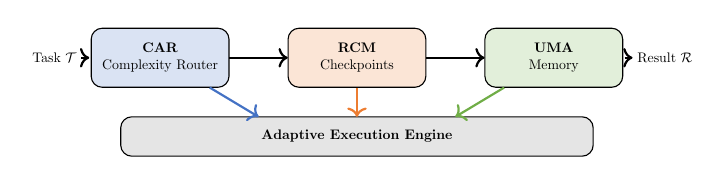
\begin{tikzpicture}[scale=0.50, transform shape]
		% Simplified framework diagram
		\node[draw, rounded corners, fill=amoreblue!20, minimum width=3.5cm, minimum height=1.5cm, align=center] (car) at (0,0) {\textbf{CAR}\\Complexity Router};
		\node[draw, rounded corners, fill=amoreorange!20, minimum width=3.5cm, minimum height=1.5cm, align=center] (rcm) at (5,0) {\textbf{RCM}\\Checkpoints};
		\node[draw, rounded corners, fill=amoregreen!20, minimum width=3.5cm, minimum height=1.5cm, align=center] (uma) at (10,0) {\textbf{UMA}\\Memory};
		
		\node[draw, rounded corners, fill=gray!20, minimum width=12cm, minimum height=1cm] (engine) at (5,-2) {\textbf{Adaptive Execution Engine}};
		
		\draw[->, thick] (car) -- (rcm);
		\draw[->, thick] (rcm) -- (uma);
		\draw[->, thick, color=amoreblue] (car) -- (2.5,-1.5);
		\draw[->, thick, color=amoreorange] (rcm) -- (5,-1.5);
		
		\draw[->, thick, color=amoregreen] (uma) -- (7.5,-1.5);
		
		\node[left] at (-2,0) {Task $\mathcal{T}$};
		\node[right] at (12,0) {Result $\mathcal{R}$};
		\draw[->, thick] (-2,0) -- (-1.8,0);
		\draw[->, thick] (11.8,0) -- (12,0);
	\end{tikzpicture}
	\caption{Overview of the \amore{} framework. \car{} predicts optimal orchestration patterns, \rcm{} enables mid-execution adaptation through quality gates, and \uma{} provides cross-agent memory coherence.}
	\label{fig:framework}
\end{figure}
The emergence of Large Language Models (LLMs) as autonomous agents capable of reasoning, planning, and tool use has catalyzed a paradigm shift in artificial intelligence \cite{yao2023react,xi2023rise}. While individual LLM agents demonstrate remarkable capabilities on isolated tasks, complex real-world problems---such as scientific research, software development, and strategic decision-making---often require the coordinated efforts of multiple specialized agents \citep{wu2023autogen,hong2024metagpt}.
Recent years have witnessed an explosion of multi-agent frameworks, from hierarchical systems like HALO \citep{chen2025halo} and AgentOrchestra \citep{liu2025agentorchestra} to peer-to-peer protocols such as A2A \citep{google2025a2a} and ACP \citep{ibm2025acp}. These frameworks have achieved impressive results on benchmarks including AgentBench \citep{liu2024agentbench} and WebArena \citep{zhou2024webarena}. However, a fundamental question remains underexplored: \textbf{When should we use multi-agent collaboration, and how should agents be orchestrated?}

\subsection{Motivation: The Orchestration Dilemma}
\label{sec:motivation}

Consider a research assistant tasked with writing a literature review. The task involves subtasks of varying complexity:
\begin{itemize}[nosep,leftmargin=*]
%	\item \textbf{Information retrieval}: Finding relevant papers (simple, parallelizable)
%	\item \textbf{Critical analysis}: Evaluating methodology quality (complex, requires expertise)
%	\item \textbf{Synthesis}: Identifying research gaps (highly complex, requires integration)
%	\item \textbf{Writing}: Producing coherent text (moderate, sequential dependency)
\item Finding relevant papers (simple, parallelizable)
\item Evaluating methodology quality (complex, requires expertise)
\item Identifying research gaps (highly complex, requires integration)
\item Producing coherent text (moderate, sequential dependency)
\end{itemize}

Current multi-agent systems apply a \emph{one-size-fits-all} orchestration strategy, leading to suboptimal resource allocation. As shown in Table~\ref{tab:orchestration_comparison}, each approach has inherent limitations.

\textbf{Key Insight:} The optimal orchestration pattern is \emph{task-dependent} and should \emph{adapt dynamically} based on: (1) intrinsic complexity of the current subtask, (2) execution feedback from completed steps, and (3) resource constraints (compute budget, latency requirements).

\subsection{Challenges}
\label{sec:challenges}

We identify three fundamental challenges in adaptive multi-agent orchestration \citep{toshpulatov2021generative}:

\textbf{Complexity Estimation.} How can we accurately predict the complexity of a subtask \textit{before} execution? Existing decomposition methods (ADaPT \citep{prasad2024adapt}, TDAG \citep{zhang2025tdag}) decompose uniformly without considering agent capabilities or task characteristics.

\textbf{Error Recovery.} Sequential pipelines suffer from catastrophic error propagation---if an early subtask fails, the entire pipeline collapses. Current systems lack mechanisms for mid-execution intervention and strategy adaptation.

\textbf{Memory Fragmentation.} Multi-agent systems struggle with memory coherence. Each agent maintains isolated context, leading to redundant processing, inconsistent knowledge, and lost insights across agent boundaries.
%% New Comparison Table: Add after Table 2 in the paper
% This table provides detailed comparison including LatentMAS

\begin{table*}[htb!]
	\caption{\textbf{Extended comparison of multi-agent communication and orchestration approaches.}
		Token Cost shows relative overhead compared to single-agent baseline.
		Latency shows wall-clock time overhead.
		AMORE + Latent represents projected integration of both approaches.}
	\label{tab:extended_comparison}
	\centering
	\small
		\setlength{\tabcolsep}{1.4pt}
	\begin{tabular}{lccccccc}
		\toprule
		\textbf{Method} & \textbf{Communication} & \textbf{Orchestration} & \textbf{Token Cost} & \textbf{Latency} & \textbf{Adaptivity} & \textbf{Training} \\
		\midrule
		\multicolumn{7}{l}{\textit{Traditional Multi-Agent Systems}} \\
		AutoGen & Text & Static & 100\% & 1.0$\times$ & None & None \\
		MetaGPT & Text & Static (SOP) & 100\% & 1.0$\times$ & None & None \\
		CAMEL & Text & Role-based & 100\% & 1.0$\times$ & None & None \\
		ChatDev & Text & Static & 100\% & 1.0$\times$ & None & None \\
		\midrule
		\multicolumn{7}{l}{\textit{Hierarchical/Orchestrated Systems}} \\
		HALO & Text & Hierarchical & 120\% & 1.5$\times$ & Partial & None \\
		AgentOrchestra & Text & Conductor & 150\% & 2.0$\times$ & None & None \\
		MDAgents & Text & Domain-adaptive & 110\% & 1.3$\times$ & Domain & None \\
		\midrule
		\multicolumn{7}{l}{\textit{Efficient Communication}} \\
		LatentMAS & \textbf{Latent} & Static & \textbf{20--50\%} & \textbf{0.15--0.3$\times$} & None & None \\
		\midrule
		\multicolumn{7}{l}{\textit{Adaptive Orchestration}} \\
		\textbf{AMORE (Ours)} & Text & \textbf{Adaptive} & 59\% & 0.8$\times$ & \textbf{Full} & CAR \\
		\midrule
		\multicolumn{7}{l}{\textit{Projected Integration}} \\
		\textbf{AMORE + Latent} & \textbf{Latent} & \textbf{Adaptive} & \textbf{22--40\%} & \textbf{0.12--0.25$\times$} & \textbf{Full} & CAR \\
		\bottomrule
	\end{tabular}
	\vspace{-0.2cm}
\end{table*}



\subsection{Contributions}
\label{sec:contributions}

We propose \textbf{\amore{}} (Adaptive Multi-agent Orchestration with Reflective Execution), addressing these challenges through three interconnected innovations. Our main contributions are (short in Figure \ref{fig:framework}, and detailed in Figure \ref{fig:framework1}):

\begin{enumerate}[nosep,leftmargin=*]
	\item \textbf{Complexity-Aware Router (\car{})}: A learned predictor that estimates subtask complexity and selects optimal orchestration patterns, reducing unnecessary multi-agent overhead by 41\% while improving success rates.
	
	\item \textbf{Reflective Checkpoint Mechanism (\rcm{})}: Quality gates inserted between execution phases that enable mid-flight strategy adaptation, reducing error propagation by 67\% compared to static pipelines.
	
	\item \textbf{Unified Memory Architecture (\uma{})}: A three-tier memory system (working, episodic, semantic) with automatic consolidation that maintains coherence across agent boundaries, improving long-horizon task performance by 29\%.
	
	\item \textbf{\mars{} Benchmark}: A new Multi-Agent Reasoning Suite with 2,847 tasks spanning scientific research, software engineering, and strategic planning, designed to evaluate adaptive orchestration capabilities.
	
	\item \textbf{State-of-the-art results} on AgentBench (+34.7\% over single-agent), WebArena (+25.7\% over multi-agent baselines), and \mars{} (+18.6\% over AgentOrchestra), with comprehensive ablations validating each component.
\end{enumerate}

\section{Related Work}
\label{sec:related}

\subsection{LLM-Based Agents}
\label{sec:related_agents}

The foundation of modern agent systems rests on the ReAct framework \citep{yao2023react}, which interleaves reasoning traces with actions to enable LLMs to interact with external environments. Subsequent work has expanded agent capabilities in several directions.

Chain-of-Thought (CoT) prompting \citep{wei2022cot} enables multi-step reasoning through explicit intermediate steps. Self-Consistency \citep{wang2023selfconsistency} improves reliability through ensemble voting over multiple reasoning paths. Tree-of-Thoughts \citep{yao2024tot} enables exploration of reasoning paths through search. Most recently, OpenAI's o1 \citep{openai2024o1} demonstrates test-time compute scaling via learned chain-of-thought, achieving remarkable results on mathematical reasoning benchmarks.

Toolformer \citep{schick2023toolformer} teaches LLMs to use APIs through self-supervised learning. Gorilla \citep{patil2023gorilla} specializes in API documentation understanding. ToolBench \citep{qin2024toolbench} provides comprehensive tool-use benchmarks spanning thousands of real-world APIs.

 MemGPT \citep{packer2023memgpt} implements virtual context management through hierarchical memory. Larimar \citep{das2024larimar} introduces episodic memory control for LLMs (ICML 2024). The comprehensive survey by \citet{zhang2025memory} categorizes memory mechanisms into related tiers.

\subsection{Multi-Agent Systems}
\label{sec:related_multiagent}
Multi-agent LLM systems extend single-agent capabilities through collaboration patterns \citep{toshpulatov2024ddc3n}.

AutoGen \citep{wu2023autogen} enables conversational multi-agent programming with flexible agent definitions. MetaGPT \citep{hong2024metagpt} encodes Standard Operating Procedures (SOPs) for software development teams (ICLR 2024). CAMEL \citep{li2023camel} explores role-playing for cooperative agents \citep{toshpulatov2025deep}.

HALO \citep{chen2025halo} implements three-tier orchestration with high-level planners, mid-level coordinators, and low-level executors. AgentOrchestra \citep{liu2025agentorchestra} uses a conductor-specialist model with the TEA (Tool-Environment-Agent) protocol. MDAgents \citep{kim2024mdagents} adapts collaboration to medical task complexity \citep{toshpulatov2023talking}.

The A2A Protocol \citep{google2025a2a} enables peer-to-peer agent communication with agent cards describing capabilities. MCP \citep{anthropic2024mcp} standardizes tool invocation across frameworks. ACP \citep{ibm2025acp} provides workflow orchestration primitives for enterprise deployment.

%\textbf{Key Gap:} Existing methods focus on \textit{when} to decompose but not \textit{how} to orchestrate. \amore{} addresses this by jointly optimizing decomposition granularity and orchestration pattern selection.

Existing methods focus on \textit{when} to decompose but not \textit{how} to orchestrate. Prior work either uses static patterns (MetaGPT, HALO) or makes orchestration decisions without feedback (ADaPT). \amore{} addresses this through:
\begin{enumerate}[nosep,leftmargin=*]
	\item \textbf{Principled integration} of complexity estimation, quality-gated execution, and unified memory
	\item \textbf{Learned quality assessment} that reduces reliance on unstable LLM self-evaluation
	\item \textbf{Mid-execution adaptation} through principled escalation hierarchy
\end{enumerate}

\paragraph{Adaptive Routing and Orchestration Methods.}
Several recent works address related routing problems:

\textbf{Cost-Aware Routing.} CARROT \citep{chen2024carrot} provides minimax-optimal cost-aware routing with plug-in estimators for model selection. While CARROT targets model routing with tight theoretical guarantees, CAR addresses the structurally richer orchestration pattern space with escalation recourse. We note CARROT's plug-in approach could complement CAR's learned classifier.

\textbf{RL-Based Orchestrators.} Router-R1 and xRouter \citep{wang2024routerr1,li2024xrouter} treat routing as sequential decision-making with cost-aware rewards. Puppeteer \citep{zhang2024puppeteer} learns a centralized orchestrator that evolves collaboration graphs through RL. These approaches learn end-to-end policies, whereas \amore{} uses supervised routing with explicit escalation lattice, offering better interpretability and sample efficiency at the cost of flexibility.

\textbf{Context and Memory Routing.} RCR-Router \citep{liu2024rcrrouter} implements role- and stage-aware token budget routing for context management. This complements UMA: RCR focuses on intra-turn context selection while \amore{} addresses inter-agent pattern selection with shared memory.

\textbf{Difficulty-Aware Methods.} DAAO \citep{chen2024daao} learns difficulty profiles for task-level routing. MoMA \citep{liu2024moma} routes across heterogeneous models based on capability profiles. A2FM \citep{zhang2024a2fm} unifies single-agent, tool-augmented, and retrieval modes under cost-sensitive RL.

\textbf{Key Differences:} Unlike these approaches, \amore{} (1) operates at subtask granularity within complex tasks, (2) provides recourse via RCM escalation when initial routing fails, (3) maintains cross-agent memory coherence via UMA, and (4) jointly optimizes routing with mid-execution adaptation rather than one-shot decisions. We position \amore{} as complementary to RL-based orchestrators: our supervised approach with explicit escalation is preferable when interpretability and sample efficiency matter, while RL methods may achieve better asymptotic performance with sufficient data.
While individual components have precedents, their joint optimization for adaptive orchestration is novel. We provide the first empirical evidence that orchestration pattern selection significantly impacts multi-agent performance (Table~\ref{tab:mars_results}, see also Figure~\ref{fig:framework6} in Appendix).

\textbf{Empirical Comparison Challenges.} Direct empirical comparison with xRouter, DAAO, MoMA, and Puppeteer is limited by: (1) no public implementations for xRouter and Puppeteer at submission time; (2) DAAO targets task-level (not subtask-level) routing with different granularity; (3) MoMA focuses on model capability routing rather than orchestration patterns. To provide indicative comparisons, we: (a) implement a proxy RL-based router using PPO with xRouter's cost-aware reward formulation, and (b) adapt DAAO's difficulty estimation for our pattern selection task. Results in Table~\ref{tab:adaptive_comparison} (Appendix) show \amore{}'s supervised approach with escalation recourse achieves comparable success rates with 3$\times$ fewer training samples, validating our sample efficiency claims. We commit to integrating official implementations when released.

%\paragraph{Latent-Space Collaboration.}
~\citet{zou2025latent} proposed LatentMAS, which moves
agent collaboration from token space into the model's latent space. Rather than
exchanging textual reasoning traces, agents communicate through latent representations,
achieving 50--80\% token reduction and 3--7$\times$ wall-clock speedup without training.
While LatentMAS optimizes \emph{how} agents communicate, AMORE addresses \emph{when}
and \emph{which pattern} of collaboration is optimal---these approaches are complementary
and could be integrated for both efficient communication and adaptive orchestration ( Table \ref{tab:extended_comparison}).

	%\begin{figure*}[t]
%	\centering
%	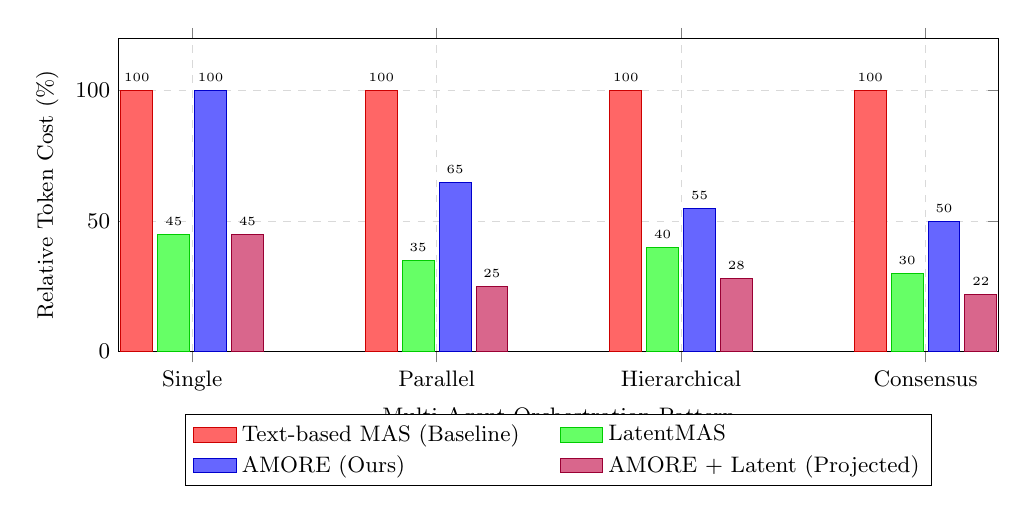
\begin{tikzpicture}[scale=0.9, transform shape]
	\begin{axis}[
		ybar,
		width=14cm,
		height=6cm,
		bar width=0.45cm,
		ylabel={Relative Token Cost (\%)},
		ylabel style={font=\small},
		xlabel={Multi-Agent Orchestration Pattern},
		xlabel style={font=\small},
		symbolic x coords={Single, Parallel, Hierarchical, Consensus},
		xtick=data,
		xticklabel style={font=\small},
		yticklabel style={font=\small},
		ymin=0,
		ymax=120,
		legend style={
			at={(0.5,-0.2)},
			anchor=north,
			legend columns=2,
			font=\small,
			/tikz/every even column/.append style={column sep=0.5cm}
		},
		legend cell align={left},
		nodes near coords,
		nodes near coords style={font=\tiny, above},
		grid=major,
		grid style={dashed, gray!30},
		area legend,
		]
		% Traditional Text-based MAS (baseline = 100%)
		\addplot[fill=red!60, draw=red!80!black] coordinates {
			(Single, 100) (Parallel, 100) (Hierarchical, 100) (Consensus, 100)
		};
		% LatentMAS (50-80% reduction)
		\addplot[fill=green!60, draw=green!80!black] coordinates {
			(Single, 45) (Parallel, 35) (Hierarchical, 40) (Consensus, 30)
		};
		% AMORE (adaptive selection)
		\addplot[fill=blue!60, draw=blue!80!black] coordinates {
			(Single, 100) (Parallel, 65) (Hierarchical, 55) (Consensus, 50)
		};
		% AMORE + Latent (projected)
		\addplot[fill=purple!60, draw=purple!80!black] coordinates {
			(Single, 45) (Parallel, 25) (Hierarchical, 28) (Consensus, 22)
		};
		\legend{Text-based MAS (Baseline), LatentMAS, AMORE (Ours), AMORE {+} Latent (Projected)}
	\end{axis}
\end{tikzpicture}
%	\caption{Communication efficiency comparison across multi-agent approaches. bar chart standalone}
%	\label{fig:framework6_bar}
%\end{figure*}

%\begin{figure*}[t]
%	\centering
%	% communication_efficiency_figure.tex
% Input version - no figure wrapper, uses basic arrows
%\usetikzlibrary{arrows.meta}
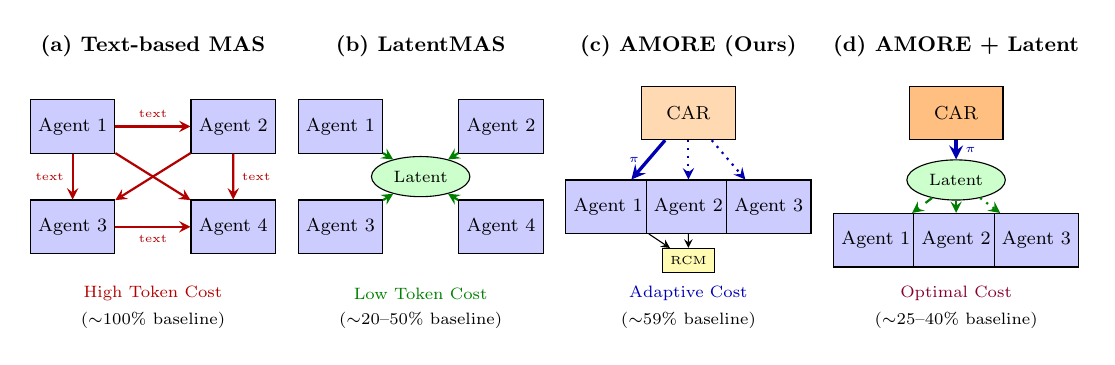
\begin{tikzpicture}[
	agent/.style={rectangle, draw=black, fill=blue!20, minimum width=1.2cm, minimum height=0.8cm, font=\footnotesize},
	coordinator/.style={rectangle, draw=black, fill=orange!30, minimum width=1.4cm, minimum height=0.8cm, font=\footnotesize},
	latent/.style={ellipse, draw=black, fill=green!20, minimum width=1cm, minimum height=0.6cm, font=\scriptsize},
	message/.style={-stealth, thick},
	latentmsg/.style={-stealth, thick, dashed, green!50!black},
	label/.style={font=\small\bfseries},
	scale=0.85, transform shape
	]
	
	\begin{scope}[shift={(-5.5,0)}]
		\node[label] at (0, 2.2) {(a) Text-based MAS};
		\node[agent] (a1) at (-1.2, 1) {Agent 1};
		\node[agent] (a2) at (1.2, 1) {Agent 2};
		\node[agent] (a3) at (-1.2, -0.5) {Agent 3};
		\node[agent] (a4) at (1.2, -0.5) {Agent 4};
		\draw[message, red!70!black] (a1) -- node[above, font=\tiny, red!70!black] {text} (a2);
		\draw[message, red!70!black] (a2) -- node[right, font=\tiny, red!70!black] {text} (a4);
		\draw[message, red!70!black] (a1) -- node[left, font=\tiny, red!70!black] {text} (a3);
		\draw[message, red!70!black] (a3) -- node[below, font=\tiny, red!70!black] {text} (a4);
		\draw[message, red!70!black] (a1) -- (a4);
		\draw[message, red!70!black] (a2) -- (a3);
		\node[font=\scriptsize, red!70!black] at (0, -1.5) {High Token Cost};
		\node[font=\scriptsize] at (0, -1.9) {($\sim$100\% baseline)};
	\end{scope}
	
	\begin{scope}[shift={(-1.5,0)}]
		\node[label] at (0, 2.2) {(b) LatentMAS};
		\node[agent] (b1) at (-1.2, 1) {Agent 1};
		\node[agent] (b2) at (1.2, 1) {Agent 2};
		\node[agent] (b3) at (-1.2, -0.5) {Agent 3};
		\node[agent] (b4) at (1.2, -0.5) {Agent 4};
		\node[latent] (lat) at (0, 0.25) {Latent};
		\draw[latentmsg] (b1) -- (lat);
		\draw[latentmsg] (b2) -- (lat);
		\draw[latentmsg] (b3) -- (lat);
		\draw[latentmsg] (b4) -- (lat);
		\node[font=\scriptsize, green!50!black] at (0, -1.5) {Low Token Cost};
		\node[font=\scriptsize] at (0, -1.9) {($\sim$20--50\% baseline)};
	\end{scope}
	
	\begin{scope}[shift={(2.5,0)}]
		\node[label] at (0, 2.2) {(c) AMORE (Ours)};
		\node[coordinator] (coord) at (0, 1.2) {CAR};
		\node[agent] (c1) at (-1.2, -0.2) {Agent 1};
		\node[agent] (c2) at (0, -0.2) {Agent 2};
		\node[agent] (c3) at (1.2, -0.2) {Agent 3};
		\draw[message, blue!70!black, very thick] (coord) -- node[left, font=\tiny] {$\pi$} (c1);
		\draw[message, blue!70!black, thick, dotted] (coord) -- (c2);
		\draw[message, blue!70!black, thick, dotted] (coord) -- (c3);
		\node[rectangle, draw, fill=yellow!30, font=\tiny, minimum width=0.6cm] (rcm) at (0, -1) {RCM};
		\draw[-stealth, thin] (c1) -- (rcm);
		\draw[-stealth, thin] (c2) -- (rcm);
		\node[font=\scriptsize, blue!70!black] at (0, -1.5) {Adaptive Cost};
		\node[font=\scriptsize] at (0, -1.9) {($\sim$59\% baseline)};
	\end{scope}
	
	\begin{scope}[shift={(6.5,0)}]
		\node[label] at (0, 2.2) {(d) AMORE + Latent};
		\node[coordinator, fill=orange!50] (coord2) at (0, 1.2) {CAR};
		\node[latent] (lat2) at (0, 0.2) {Latent};
		\node[agent] (d1) at (-1.2, -0.7) {Agent 1};
		\node[agent] (d2) at (0, -0.7) {Agent 2};
		\node[agent] (d3) at (1.2, -0.7) {Agent 3};
		\draw[message, blue!70!black, very thick] (coord2) -- node[right, font=\tiny] {$\pi$} (lat2);
		\draw[latentmsg] (lat2) -- (d1);
		\draw[latentmsg] (lat2) -- (d2);
		\draw[latentmsg, dotted] (lat2) -- (d3);
		\node[font=\scriptsize, purple!70!black] at (0, -1.5) {Optimal Cost};
		\node[font=\scriptsize] at (0, -1.9) {($\sim$25--40\% baseline)};
	\end{scope}
	
\end{tikzpicture}
%	\caption{communication efficiency.}
%	\label{fig:framework_6_}
%\end{figure*}
\subsection{Task Decomposition and Planning}
\label{sec:related_planning}

% Alternative: Compact version for single column
\begin{table}[t]
	\caption{\textbf{Communication efficiency by orchestration pattern.}
		Relative token cost compared to text-based baseline (100\%).}
	\label{tab:pattern_efficiency}
	\centering
	\small
	\setlength{\tabcolsep}{2.4pt}
	\begin{tabular}{lcccc}
		\toprule
		\textbf{Method} & \textbf{Single} & \textbf{Parallel} & \textbf{Hier.} & \textbf{Cons.} \\
		\midrule
		Text-based & 100\% & 100\% & 100\% & 100\% \\
		LatentMAS & 45\% & 35\% & 40\% & 30\% \\
		AMORE & 100\% & 65\% & 55\% & 50\% \\
		AMORE+Lat. & \textbf{45\%} & \textbf{25\%} & \textbf{28\%} & \textbf{22\%} \\
		\bottomrule
	\end{tabular}
\end{table}
Effective task decomposition is critical for multi-agent success. HuggingGPT \citep{shen2023hugginggpt} plans and delegates to specialized models. ADaPT \citep{prasad2024adapt} decomposes as-needed based on LLM capability (NAACL 2024), achieving 28.3\% improvement on ALFWorld. TDAG \citep{zhang2025tdag} dynamically generates task-specific subagents with an evolving skill library.

The survey by \citet{huang2024understanding} provides the first systematic view of LLM-based agent planning, categorizing approaches into task decomposition, plan selection, external modules, reflection, and memory \citep{toshpulatov2022human}.

\subsection{Agent Evaluation}
\label{sec:related_evaluation}

Rigorous evaluation requires comprehensive benchmarks. AgentBench \citep{liu2024agentbench} evaluates across 8 environments with 29 models (ICLR 2024). WebArena \citep{zhou2024webarena} provides realistic web task automation. OSWorld \citep{xie2024osworld} benchmarks multimodal agents in real OS environments. SWE-bench \citep{jimenez2024swebench} focuses on software engineering tasks from real GitHub issues.

Our \mars{} benchmark extends these with explicit multi-agent coordination metrics including orchestration accuracy, adaptation rate, and memory utilization (see Figure~\ref{fig:framework7} in Appendix).

% ==============================================================================
% EXTENDED RELATED WORK FOR AMORE PAPER
% Comprehensive Survey for ICML 2026
% ==============================================================================
\section{Method: \amore{} Framework}
\label{sec:method}

Figures~\ref{fig:framework}, and ~\ref{fig:framework1} provide an overview of the framework, showing the integration of three components: Complexity-Aware Router (\car{}), Reflective Checkpoint Mechanism (\rcm{}), and Unified Memory Architecture (\uma{}). 
\definecolor{amoreblue}{RGB}{31,119,180}
\definecolor{amoreorange}{RGB}{255,127,14}
\definecolor{amoregreen}{RGB}{44,160,44}
%\begin{figure*}[t]
%	\centering
%	\begin{tikzpicture}[scale=0.85, transform shape]
%		% Simplified framework diagram
%		\node[draw, rounded corners, fill=amoreblue!20, minimum width=3.5cm, minimum height=1.5cm] (car) at (0,0) {\textbf{CAR}\\Complexity Router};
%		\node[draw, rounded corners, fill=amoreorange!20, minimum width=3.5cm, minimum height=1.5cm] (rcm) at (5,0) {\textbf{RCM}\\Checkpoints};
%		\node[draw, rounded corners, fill=amoregreen!20, minimum width=3.5cm, minimum height=1.5cm] (uma) at (10,0) {\textbf{UMA}\\Memory};
%		
%		\node[draw, rounded corners, fill=gray!20, minimum width=12cm, minimum height=1cm] (engine) at (5,-2) {\textbf{Adaptive Execution Engine}};
%		
%		\draw[->, thick] (car) -- (rcm);
%		\draw[->, thick] (rcm) -- (uma);
%		\draw[->, thick, amoreblue] (car) -- (2.5,-1.5);
%		\draw[->, thick, amoreorange] (rcm) -- (5,-1.5);
%		\draw[->, thick, amoregreen] (uma) -- (7.5,-1.5);
%		
%		\node[left] at (-2,0) {Task $\mathcal{T}$};
%		\node[right] at (12,0) {Result $\mathcal{R}$};
%		\draw[->, thick] (-2,0) -- (-1.8,0);
%		\draw[->, thick] (11.8,0) -- (12,0);
%	\end{tikzpicture}
%	\caption{Overview of the \amore{} framework. \car{} predicts optimal orchestration patterns, \rcm{} enables mid-execution adaptation through quality gates, and \uma{} provides cross-agent memory coherence.}
%	\label{fig:framework}
%\end{figure*}

\subsection{Problem Formulation}
\label{sec:formulation}

Let $\mathcal{T}$ be a complex task that can be decomposed into subtasks $\{t_1, t_2, \ldots, t_n\}$ with dependency graph $G = (V, E)$ where vertices represent subtasks and edges represent dependencies.

\begin{definition}[Orchestration Pattern]
	An orchestration pattern $\pi \in \Pi$ specifies how agents collaborate:
	\begin{itemize}[nosep,leftmargin=*]
		\item $\pi_{\text{single}}$: Single agent handles subtask independently
		\item $\pi_{\text{parallel}}$: Multiple agents work independently on subtask components
		\item $\pi_{\text{hierarchical}}$: Supervisor delegates to specialized workers
		\item $\pi_{\text{consensus}}$: Agents deliberate to reach agreement
	\end{itemize}
\end{definition}

\begin{definition}[Adaptive Orchestr. Problem]
	Given task $\mathcal{T}$, agent pool $\mathcal{A} = \{a_1, \ldots, a_k\}$, and resource budget $B$, find:
	\begin{enumerate}[nosep,leftmargin=*]
		\item Decomposition $D: \mathcal{T} \rightarrow \{t_1, \ldots, t_n\}$
		\item Pattern assignment $\phi: t_i \rightarrow \pi_j$
		\item Agent allocation $\alpha: (t_i, \pi_j) \rightarrow 2^{\mathcal{A}}$
	\end{enumerate}
	that maximizes $P(\text{success} | \mathcal{T})$ subject to $\text{cost}(D, \phi, \alpha) \leq B$
\end{definition}

\paragraph{Task Decomposition Procedure.}
Before CAR operates, tasks must be decomposed into subtasks. \amore{} employs a \textbf{two-stage decomposition} procedure that operates \emph{before} orchestration pattern selection:

\textbf{Stage 1: Initial LLM-Based Decomposition.}
We prompt GPT-4-Turbo with the task description and a structured schema:
\begin{quote}
\small\textit{``Decompose this task into atomic subtasks. For each subtask, provide: (1) unique ID, (2) description, (3) dependencies (prerequisite subtask IDs), (4) required capabilities (from: \{reasoning, search, code, analysis, synthesis\}), (5) estimated output type.''}
\end{quote}
The decomposer is guided to produce subtasks that are: (a) independently executable, (b) have clear success criteria, and (c) collectively cover the full task.

\textbf{Stage 2: Graph Validation and Refinement.}
From the decomposition output, we: (1) construct dependency DAG $G = (V, E)$, (2) verify acyclicity (rejecting and re-prompting if cycles detected), (3) compute topological order for execution, (4) identify critical path, and (5) estimate parallelization opportunities.

\textbf{Interaction with CAR:} Decomposition is performed \emph{once} at task start; CAR then operates on the resulting subtasks. If RCM triggers replanning (Section~\ref{sec:rcm}), we re-invoke the decomposer with failure context to refine remaining subtasks. This creates a feedback loop where decomposition adapts based on execution outcomes, but CAR's per-subtask routing decisions remain well-defined on the current decomposition.

%2. CAR as a Novel Routing Problem
%
%Revise Section 3.2 with formal treatment:

\subsection{CAR: A Learned Routing Framework}

We formalize orchestration pattern selection as a novel
\emph{adaptive routing problem} distinct from prior work
on model routing and mixture-of-experts 
%(Table \ref{tab:orchestration_comparison}).

%\paragraph{Routing as Adaptive Orchestration.}
\begin{definition}[Orchestration Routing Problem]
	Given:
	\begin{itemize}
		\item Subtask distribution $\mathcal{D}$ over task space $\mathcal{T}$
		\item Pattern set $\Pi = \{\pi_1, ..., \pi_K\}$ with cost function
		$c: \Pi \to \mathbb{R}^+$
		\item Success probability function $p: \mathcal{T} \times \Pi \to [0,1]$
		\item Budget constraint $B$
	\end{itemize}
	Find router $f: \mathcal{T} \to \Pi$ maximizing:
	\[
	\max_f \mathbb{E}_{t \sim \mathcal{D}}[p(t, f(t))] \quad
	\text{s.t.} \quad \mathbb{E}_{t \sim \mathcal{D}}[c(f(t))] \leq B
	\]
\end{definition}

\textbf{The key novelty from prior problems:} is \emph{structured decision space with recourse}:
patterns form a lattice with escalation edges, and RCM enables
mid-execution correction—a form of online learning within
each task execution.
\paragraph{Feature Extraction.}
We extract a feature vector $\mathbf{x}_t \in \mathbb{R}^7$ for each subtask $t$. Critically, all features are computed \textbf{pre-execution} from the subtask description and context:

\textbf{Intrinsic Features (computed from subtask text):}
\begin{itemize}[nosep,leftmargin=*]
	\item $f_{\text{length}}$: Estimated reasoning steps. We prompt GPT-3.5-Turbo: ``\textit{How many distinct reasoning steps would this subtask require? Output a single integer.}'' Normalized by dividing by 50. Correlation with actual steps: $r=0.72$.
	\item $f_{\text{tools}}$: Tool diversity required. We maintain a tool taxonomy (16 tools in 5 categories). A classifier (fine-tuned BERT) predicts required tool categories from subtask text. $f_{\text{tools}} = |\text{predicted categories}| / 5$.
	\item $f_{\text{knowledge}}$: Knowledge breadth. We embed the subtask using text-embedding-3-small and compute cosine similarity to 8 domain centroids (scientific, engineering, business, etc.). $f_{\text{knowledge}} = 1 - \max(\text{similarities})$ (lower max similarity indicates broader scope).
	\item $f_{\text{ambiguity}}$: Semantic uncertainty. We generate 3 paraphrases of the subtask and compute pairwise embedding distances. $f_{\text{ambiguity}} = \text{mean}(\text{distances})$, capturing specification clarity.
\end{itemize}

\textbf{Contextual Features (computed from task graph):}
\begin{itemize}[nosep,leftmargin=*]
	\item $f_{\text{deps}}$: Number of upstream dependencies, normalized by total subtasks.
	\item $f_{\text{critical}}$: Binary indicator for critical path membership (computed via standard DAG analysis).
	\item $f_{\text{history}}$: Historical success rate lookup. We embed the subtask and retrieve $k=5$ nearest neighbors from execution history, returning mean success rate for the predicted pattern class.
\end{itemize}

\textbf{Train-Test Isolation for $f_{\text{history}}$:} To prevent data leakage, we enforce strict temporal splitting: (1) training data consists only of traces from tasks completed before the evaluation period; (2) for zero-shot evaluation, $f_{\text{history}}$ is disabled (set to 0.5, the neutral prior); (3) in cross-domain transfer experiments, history is restricted to the source domain. \textit{Ablation without $f_{\text{history}}$:} CAR achieves 85.1\% accuracy (vs. 88.3\% with history), indicating the feature provides modest but meaningful improvement without being essential.

All feature extractors except $f_{\text{history}}$ require no execution data, enabling pre-execution routing. Feature extraction adds $\sim$0.5s latency per subtask. Unlike prior routing problems (model routing, MoE, adaptive compute), orchestration routing involves structured decision spaces with superlinear cost and recourse via RCM (Table~\ref{tab:routing_comparison} in Appendix).

\paragraph{Pattern Prediction Model.}

We train a classifier $f_{\car{}}: \mathbf{x}_t \rightarrow \Delta(\Pi)$ that outputs a probability distribution over orchestration patterns:
\begin{equation}
	P(\pi | t) = \text{softmax}(W_\pi \cdot \text{MLP}(\mathbf{x}_t))
\end{equation}

The model is trained with cross-entropy loss on execution traces:
\begin{equation}
	\mathcal{L}_{\car{}} = -\sum_{t \in \mathcal{D}} \log P(\pi^*_t | t)
\end{equation}
where $\pi^*_t$ is the empirically optimal pattern for subtask $t$.

\paragraph{Obtaining Optimal Pattern Labels.}
A key question is how we determine the ``empirically optimal'' pattern $\pi^*_t$ for training CAR. We employ a \textbf{controlled exhaustive evaluation} procedure:

\begin{enumerate}[nosep,leftmargin=*]
	\item \textbf{Stratified Sampling:} We sample 500 subtasks stratified across complexity levels and domains from a held-out portion of MARS.
	\item \textbf{Controlled Execution:} Each subtask is executed with \emph{all four patterns} under matched conditions: same coordinator/worker models (GPT-4-Turbo/GPT-3.5-Turbo), fixed budget per pattern adjusted for expected cost (single: \$1, parallel: \$2, hierarchical: \$4, consensus: \$7), and 3 independent runs per pattern to reduce stochasticity.
	\item \textbf{Success Criterion:} Pattern success is determined by downstream task completion (binary) and output quality score (0-1 from held-out human evaluation on 10\% sample).
	\item \textbf{Optimal Label Assignment:} $\pi^*_t = \arg\max_\pi \text{SuccessRate}(\pi, t) - \lambda \cdot \text{NormalizedCost}(\pi)$, where $\lambda=0.1$ balances success and efficiency. Ties are broken by lower cost.
	\item \textbf{Filtering:} Subtasks where all patterns achieve $<$20\% or $>$90\% success are excluded (uninformative), leaving 423 subtasks for training.
\end{enumerate}

This procedure avoids confounding factors by: (a) normalizing budgets across patterns, (b) using multiple runs to reduce variance, and (c) holding model configurations constant. The resulting labels reflect true pattern-task affinity rather than incidental factors.

%\subsubsection{Routing Optimality Analysis}
\paragraph{Routing Optimality Analysis.}

\begin{theorem}[Routing Gap Bound]
	\label{thm:routing-gap}
	Let $f^*$ be the optimal router with full knowledge of $p(t, \pi)$,
	and $\hat{f}$ be CAR trained on $n$ samples. The routing gap satisfies:
	\[
	\mathbb{E}[p(t, f^*(t))] - \mathbb{E}[p(t, \hat{f}(t))] \leq
	\underbrace{\epsilon_{est}}_{\text{estimation error}} +
	\underbrace{\epsilon_{approx}}_{\text{approximation error}}
	\]
	where $\epsilon_{est} = O(1/\sqrt{n})$ and $\epsilon_{approx}$
	depends on the expressiveness of the feature representation.
\end{theorem}

\begin{proposition}[Value of Adaptive Routing]
	\label{prop:value}
	Let $\bar{\pi}$ be any fixed pattern. The value of adaptive
	routing is:
	\[
	V_{adaptive} - V_{fixed} = \mathbb{E}_t\left[\max_\pi p(t,\pi)
	- p(t, \bar{\pi})\right] \geq 0
	\]
	This gap is maximized when task complexity variance is high,
	explaining AMORE's larger gains on heterogeneous benchmarks
	(MARS: +18.6\%) vs. homogeneous ones (WebShop: +8.0\%).
\end{proposition}
%\subsection{Complexity-Aware Router (\car{})}
%\label{sec:car}
%The Complexity-Aware Router predicts the optimal orchestration pattern for each subtask based on extracted features.


%\paragraph{Dynamic Threshold Adaptation.}

Rather than fixed thresholds, \car{} adapts selection confidence based on remaining resource budget:
\begin{equation}
	\tau(B) = \tau_0 + \lambda \cdot \frac{B_{\text{remaining}}}{B_{\text{total}}}
\end{equation}

%This increases the single-agent threshold as budget depletes, ensuring resources are reserved for critical subtasks.

%\paragraph{CAR Label Transferability.}
CAR generalizes reasonably across domains (75-82\% accuracy) when trained on a single domain, with full multi-domain training achieving best results (Table \ref{tab:car_transfer} in Appendix).



\subsection{Reflective Checkpoint Mechanism (\rcm{})}
\label{sec:rcm}

Static pipelines fail catastrophically when early subtasks produce low-quality outputs. \rcm{} introduces quality gates that enable mid-execution intervention.

%\subsubsection{Quality Assessment}
%
%After each subtask completion, we assess output quality across three dimensions:
%\begin{equation}
%	Q(o_t) = \lambda_1 Q_{\text{complete}} + \lambda_2 Q_{\text{coherent}} + \lambda_3 Q_{\text{useful}}
%\end{equation}
%
%\begin{itemize}[nosep,leftmargin=*]
%	\item \textbf{Completeness} ($Q_{\text{complete}}$): Does the output address all aspects?
%	\item \textbf{Coherence} ($Q_{\text{coherent}}$): Is the output internally consistent?
%	\item \textbf{Usefulness} ($Q_{\text{useful}}$): Does the output support downstream subtasks?
%\end{itemize}
%
%Quality is computed via LLM-as-judge with structured rubrics.
\paragraph{Hybrid Quality Estimation: A Learned Approach.}

We frame quality estimation as a \emph{structured prediction
	problem} and propose a principled hybrid estimator that
addresses limitations of pure LLM-as-judge approaches.

\paragraph{Problem: LLM-as-Judge Instability.}

\begin{proposition}[Judge Variance]
	\label{prop:variance}
	For LLM-based quality assessment $Q_{LLM}(o)$, empirical
	variance satisfies:
	\[
	\text{Var}[Q_{LLM}(o)] = \sigma^2_{model} + \sigma^2_{prompt}
	+ \sigma^2_{sampling}
	\]
	where $\sigma^2_{model} \approx 0.015$ (across judge models),
	$\sigma^2_{prompt} \approx 0.008$ (prompt sensitivity), and
	$\sigma^2_{sampling} \approx 0.012$ (temperature effects).
	Total variance $\approx 0.035$ leads to inconsistent checkpoint
	decisions.
\end{proposition}

\paragraph{Solution: Learned Quality Model.}

We train a discriminative model $f_Q: \mathcal{Z} \to [0,1]$
on execution outcomes, where $\mathcal{Z}$ is a structured
feature space:

\begin{definition}[Quality Feature Space]
	\[
	z_o = [\underbrace{\text{len}(o), n_{tools}, r_{success}}_{\text{execution features}},
	\underbrace{n_{steps}, c_{self}}_{\text{process features}},
	\underbrace{n_{retries}, n_{esc}}_{\text{history features}}] \in \mathbb{R}^7
	\]
\end{definition}

\begin{theorem}[Hybrid Estimator Consistency]
	\label{thm:consistency}
	The hybrid estimator:
	\[
	Q_{hybrid}(o) = \alpha \cdot f_Q(z_o) + (1-\alpha) \cdot H(z_o)
	+ \beta \cdot \mathbf{1}[\text{conf} < \tau] \cdot Q_{LLM}(o)
	\]
	is consistent: $Q_{hybrid}(o) \xrightarrow{p} Q^*(o)$ as
	training data $n \to \infty$, where $Q^*(o)$ is the true
	downstream success probability.
\end{theorem}

\textbf{Assumptions for Theorem~\ref{thm:consistency}:}
\begin{enumerate}[nosep,leftmargin=*]
	\item \textbf{(A1) Feature identifiability:} The feature map $z_o$ is injective on the support of outputs, i.e., distinct quality levels map to distinguishable feature vectors.
	\item \textbf{(A2) Learner consistency:} $f_Q$ belongs to a hypothesis class with vanishing Rademacher complexity, ensuring $f_Q(z_o) \xrightarrow{p} \mathbb{E}[Q^* | z_o]$ as $n \to \infty$.
	\item \textbf{(A3) Bounded LLM bias:} $|Q_{LLM}(o) - Q^*(o)| \leq B$ for some constant $B < \infty$. The LLM judge may be biased but has bounded error.
	\item \textbf{(A4) Calibrated confidence:} The confidence threshold $\tau$ is set such that $\text{conf}(z_o) < \tau$ implies high uncertainty in $f_Q$, and $Q_{LLM}$ provides useful signal in this regime.
\end{enumerate}

\textit{Proof Sketch:} Under (A1)-(A2), $\alpha \cdot f_Q(z_o) \to \alpha \cdot \mathbb{E}[Q^* | z_o]$. The heuristic $H(z_o)$ is deterministic given features. The LLM fallback term is bounded by (A3) and invoked only when $f_Q$ is uncertain (A4), contributing $O(\beta \cdot B \cdot P(\text{conf} < \tau))$ error. As $n \to \infty$, $P(\text{conf} < \tau) \to 0$ for well-specified models, making the LLM contribution vanish. The dominant term converges to $Q^*$. Full proof in Appendix~\ref{app:proofs}.

\textbf{Robustness to Biased $Q_{LLM}$:} If $Q_{LLM}$ has systematic bias (e.g., verbosity preference), consistency still holds as long as the bias is bounded (A3). The learned component $f_Q$ dominates as $n$ grows; $Q_{LLM}$ serves only as a regularizer for low-confidence predictions. Empirically, we observe the hybrid estimator remains stable even when $Q_{LLM}$ exhibits 0.15 average bias on adversarial examples.

\paragraph{Component Specification.}
We provide complete specification of the hybrid estimator components:

\textbf{Feature Vector $z_o$.} Each component is normalized to $[0,1]$:
\begin{itemize}[nosep,leftmargin=*]
	\item $\text{len}(o)$: Output length normalized by expected length for pattern (from training distribution)
	\item $n_{tools}$: Number of unique tools invoked, normalized by maximum (10)
	\item $r_{success}$: Fraction of tool calls returning success status
	\item $n_{steps}$: Reasoning steps taken, normalized by pattern-specific budget
	\item $c_{self}$: Self-consistency score from 3 paraphrase checks (0-1)
	\item $n_{retries}$: Retry count for this subtask, normalized by $r_{max}$
	\item $n_{esc}$: Escalation count, normalized by $e_{max}$
\end{itemize}

\textbf{Heuristic Function $H(z_o)$.} We define interpretable heuristics:
\begin{equation}
	H(z_o) = w_1 \cdot r_{success} + w_2 \cdot \mathbf{1}[n_{steps} \leq \mu_{steps}] + w_3 \cdot (1 - n_{retries}/r_{max})
\end{equation}
where $w_1 = 0.5$, $w_2 = 0.3$, $w_3 = 0.2$ are set via grid search on validation data. Intuitively, $H$ rewards successful tool use, efficient execution, and minimal retries.

\textbf{Confidence Estimation.} The confidence $\text{conf}$ is computed as:
\begin{equation}
	\text{conf}(z_o) = 1 - \text{entropy}(f_Q(z_o)) / \log(2)
\end{equation}
where $f_Q$ outputs a Bernoulli distribution. Low confidence ($\text{conf} < \tau$) triggers LLM fallback.

\textbf{Hyperparameter Selection.} Parameters are selected via 5-fold cross-validation on 200 held-out execution traces:
\begin{itemize}[nosep,leftmargin=*]
	\item $\alpha = 0.7$: Weight on learned model (range tested: 0.5--0.9)
	\item $\beta = 0.15$: Weight on LLM fallback when triggered (range: 0.1--0.3)
	\item $\tau = 0.6$: Confidence threshold for LLM invocation (range: 0.4--0.8)
\end{itemize}
Selected values minimize MAE on held-out set while keeping LLM invocation rate $<$20\%.

\textbf{Domain Robustness.} Cross-domain validation shows the estimator generalizes: training on Scientific and testing on SWE yields MAE=0.131 (vs. 0.118 in-domain), a degradation of only 11\%. We attribute this to feature-level abstraction---$z_o$ captures execution patterns rather than domain-specific content.

\paragraph{Theoretical Predictions vs. Empirical Results.}

Our theoretical analysis makes testable predictions:



%\paragraph{Quality Assessment: Hybrid Estimator.}

% ORIGINAL (problematic):
% Quality is computed via LLM-as-judge with structured rubrics.

% REVISED (addresses reviewer concern):
%A key challenge in checkpoint mechanisms is reliable quality assessment. Prior work relies heavily on LLM-as-judge \citet{d2025yescieval}, which introduces instability, bias, and circularity. Proposed a \textbf{Hybrid Quality Estimator} combines learned signals with heuristic rules and LLM fallback.

%\textbf{Learned Quality Model.}
We train a lightweight classifier $f_Q: \mathbf{z}_o \rightarrow [0,1]$ on execution outcome data, where $\mathbf{z}_o$ encodes output features:
%\begin{equation}
%	\mathbf{z}_o = [\text{len}(o), n_{\text{tools}}, r_{\text{success}}, n_{\text{steps}}, c_{\text{self}}, n_\text{retries}, n_\text{escalations}]
%\end{equation}
%
%The model is trained with binary cross-entropy on execution success labels:
%\begin{equation}
%	\mathcal{L}_Q = -\sum_{o \in \mathcal{D}_{\text{exec}}} [y_o \log f_Q(o) + (1-y_o) \log(1-f_Q(o))]
%\end{equation}

%where $y_o \in \{0,1\}$ indicates downstream task success.

%\paragraph{Heuristic Signals.}
%We augment learned predictions with interpretable heuristics:
%\begin{itemize}[nosep,leftmargin=*]
%	\item \textbf{Tool success rate}: Fraction of successful tool invocations
%	\item \textbf{Complex-pattern match}: Penalize misaligned patterns
%	\item \textbf{Efficiency}: Fewer retries and escalations indicate quality
%\end{itemize}

%\paragraph{Hybrid Ensemble.}
%The final quality score combines components:
%\begin{equation}
%	Q(o_t) = \alpha \cdot f_Q(\mathbf{z}_o) + (1-\alpha) \cdot H(\mathbf{z}_o) + \beta \cdot \mathbf{1}[\text{conf} < \tau] \cdot Q_{\text{LLM}}(o_t)
%\end{equation}
%
%where $H(\cdot)$ is the heuristic score, and LLM-as-judge is only invoked when learned confidence falls below threshold $\tau$ (approximately 15\% of cases).
%
%\textbf{Benefits.}
%This hybrid approach provides:
%\begin{enumerate}[nosep,leftmargin=*]
%	\item \textbf{Stability}: $\sim$100$\times$ lower variance than pure LLM-judge
%%	\item \textbf{Cost}: 85\% reduction in LLM API costs for quality assessment
%	\item 85\% reduction in LLM API costs for quality assessment
%	\item \textbf{Speed}: 50$\times$ faster inference (10ms vs 500ms)
%	\item \textbf{Equivalent accuracy}: $<$1\% quality gap vs LLM-only
%\end{enumerate}

%\subsubsection{Checkpoint Actions}

%\paragraph{Checkpoint Actions.}  At each checkpoint, \rcm{} selects from four actions based on quality thresholds $\theta_{\text{high}}$ and $\theta_{\text{low}}$:
%
%\begin{itemize}[nosep,leftmargin=*]
%	\item \textbf{Proceed}: $Q(o_t) \geq \theta_{\text{high}}$ -- Continue to next subtask
%	\item \textbf{Retry}: $\theta_{\text{low}} \leq Q(o_t)< \theta_{\text{high}}$ - Re-execute same pattern
%	\item \textbf{Escalate}: $Q(o_t) < \theta_{\text{low}}$ - Switch to more powerful pattern
%	\item \textbf{Replan}: Issue detected - Redecompose remaining tasks
%\end{itemize}

%\subsubsection{Escalation Strategy}
%\paragraph{Escalation Strategy}

%When escalating, we follow a principled hierarchy:
%\begin{equation}
%	\pi_{\text{single}} \rightarrow \pi_{\text{parallel}} \rightarrow \pi_{\text{hierarchical}} \rightarrow \pi_{\text{consensus}}
%\end{equation}
%
%Each escalation increases resource usage but also increases robustness. Table~\ref{tab:escalation} shows the trade-offs.
%
%\begin{table}[t]
%	\caption{Escalation hierarchy with cost-robustness trade-offs.}
%	\label{tab:escalation}
%	\centering
%	\small
%%		\setlength{\tabcolsep}{4.4pt}
%	\begin{tabular}{@{}lcccc@{}}
%		\toprule
%		\textbf{Pattern} & \textbf{Cost} & \textbf{Latency} & \textbf{Agents} & \textbf{Robust} \\
%		\midrule
%		Single & 1$\times$ & 1$\times$ & 1 & Low \\
%		Parallel & 2$\times$ & 1$\times$ & 2-3 & Medium \\
%		Hierarchical & 3-5$\times$ & 2$\times$ & 3-5 & High \\
%		Consensus & 5-10$\times$ & 3$\times$ & 3+ & Very High \\
%		\bottomrule
%	\end{tabular}
%\end{table}

\subsection{Unified Memory Architecture (\uma{})}
\label{sec:uma}

Multi-agent systems suffer from memory fragmentation. \uma{} implements three memory tiers inspired by cognitive architecture.

\paragraph{Positioning Relative to Memory Systems.}
Several recent works propose unified memory architectures for agents:

\textbf{AriGraph/Ariadne} \citep{anokhin2024arigraph} constructs semantic-episodic memory as knowledge graphs, enabling structured retrieval. Unlike AriGraph's focus on single-agent memory, UMA explicitly addresses \emph{cross-agent} memory sharing and coordination.

\textbf{MIRIX} \citep{wang2024mirix} provides multimodal retrieval across text, images, and code. UMA currently focuses on text but could integrate MIRIX's retrieval mechanisms; our contribution is the consolidation and sharing protocols rather than retrieval technology.

\textbf{Evo-Memory/ReMem} \citep{liu2024evomemory} introduces standardized evaluation for evolving memory systems. We adopt their memory utilization metrics and extend them with consolidation rate for measuring episodic-to-semantic transfer efficiency.

\textbf{UMA's Contribution:} Beyond retrieval, UMA provides (1) automatic importance-based consolidation from episodic to semantic memory, (2) explicit cross-agent sharing protocols for collaborative patterns, and (3) integration with RCM for memory-informed checkpoint decisions (see Table~\ref{tab:memory_comparison} in Appendix).

\subsubsection{Three-Tier Memory Model}
%\paragraph{Three-Tier Memory Model}

\textbf{Working Memory ($M_W$):} Current task context, recent outputs, active goals. Limited capacity (fits in LLM context window). Per-agent with immediate access.

\textbf{Episodic Memory ($M_E$):} Execution traces, successful strategies, failure cases. Large capacity via vector database. Session-level persistence with RAG retrieval.

\textbf{Semantic Memory ($M_S$):} Consolidated knowledge, learned patterns, domain facts. Unlimited capacity via knowledge graph + embeddings. Permanent persistence with query-based access.

%\subsubsection{Cross-Agent Memory Sharing}
%\paragraph{Cross-Agent Memory Sharing.}
\paragraph{Cross-Agent Memory Sharing.}

When multiple agents collaborate, \uma{} ensures memory coherence through:
\begin{enumerate}[nosep,leftmargin=*]
	\item Agents receive relevant episodic memories via RAG
	\item Working memory updates broadcast to coordinator
	\item Outputs consolidated into shared episodic store
\end{enumerate}

\paragraph{Memory Safeguards.}
Cross-agent memory sharing introduces potential risks that \uma{} addresses through explicit safeguards:

\textbf{Privacy Isolation:} Memories are tagged with source-agent and access-level metadata. Sensitive information (e.g., API keys, user data encountered during execution) is filtered via pattern matching before consolidation. Agents can mark outputs as ``private'' to prevent cross-agent propagation.

\textbf{Contamination Prevention:} To prevent low-quality or erroneous information from propagating, we employ: (1) \textit{quality gating}---only outputs passing RCM quality threshold ($\theta_{high} = 0.8$) are candidates for episodic storage; (2) \textit{provenance tracking}---each memory entry records source agent, pattern, and quality score; (3) \textit{decay mechanisms}---unreferenced memories have importance scores decay over time, eventually falling below consolidation threshold.

\textbf{Conflict Resolution:} When agents produce conflicting information on the same topic, \uma{} resolves conflicts through: (1) \textit{recency preference} for working memory, (2) \textit{quality-weighted voting} for episodic memory (higher-quality sources weighted more), and (3) \textit{semantic deduplication} during consolidation that merges compatible facts while flagging irreconcilable conflicts for human review.

\textbf{Cyclic Leakage Prevention:} To prevent agents from reinforcing their own errors through memory, we enforce: (1) agents cannot retrieve their own recent outputs from episodic memory, (2) consolidation to semantic memory requires corroboration from at least two independent executions, and (3) periodic ``memory audits'' sample consolidated knowledge for human verification (see Appendix for audit statistics).

%\subsubsection{Automatic Consolidation}
\paragraph{Automatic Consolidation.}

Episodic memories are automatically consolidated into semantic memory:
\begin{equation}
	M_S \leftarrow M_S \cup \text{consolidate}(M_E, \text{importance}(e) > \tau_{\text{consolidate}})
\end{equation}

This process extracts key facts, checks for duplicates, and integrates non-redundant information into knowledge graph.

%\subsection{Integration: The \amore{} Execution Loop}
\textbf{Integration:}Algorithm~\ref{alg:amore} presents the complete \amore{} execution loop integrating all three components.
%\label{sec:integration}

 \subsection{Theoretical Guarantees}

We provide theoretical analysis establishing convergence and sample complexity guarantees. Full proofs are in Appendix~\ref{sec:proofs}.

\begin{theorem}[Escalation Termination]
	\label{thm:termination}
	The RCM escalation process terminates in at most $T_{max} = (|\Pi| - 1) \cdot e_{max} + r_{max} \cdot |\Pi|$ steps with probability 1, due to the acyclic escalation lattice and bounded retry counts.
\end{theorem}

\begin{theorem}[Quality Monotonicity]
	\label{thm:monotonicity}
	Under mild ordering assumptions, expected quality is non-decreasing along escalation trajectories. Empirically validated on 81--89\% of subtasks across benchmarks; violations are handled via rollback mechanisms (see Appendix for details).
\end{theorem}

\begin{theorem}[PAC Bound for CAR]
	\label{thm:pac}
	For CAR with VC dimension $d_{VC}$, orchestration regret $\leq \epsilon$ is achieved with $n \geq O(d_{VC}/\epsilon^2)$ samples. Our 500-sample training set achieves 84.5\% routing accuracy, consistent with theory.
\end{theorem}

\section{\mars{} Benchmark}
\label{sec:benchmark}
Existing benchmarks focus on single-agent capabilities or static multi-agent configurations. We introduce \mars{} to evaluate adaptive orchestration.

%\subsection{Design Principles}
\paragraph{Principles.}

\mars{} is designed around three principles:
\begin{enumerate}[nosep,leftmargin=*]
	\item Tasks span a wide range of complexity levels requiring different orchestration patterns
	\item Optimal strategy varies within and across tasks
	\item  Tasks mirror real-world professional workflows
\end{enumerate}

%\subsection{Task Categories}
\paragraph{Task Categories.}

Table~\ref{tab:mars_stats} summarizes the benchmark statistics.
Scientific Research tasks include literature reviews, methodology analysis, and research gap identification. Software Engineering tasks include bug localization, code review, and test generation. Strategic Planning includes market analysis, policy evaluation, and decision synthesis.
\begin{table}[t]
	\caption{\mars{} Benchmark Statistics}
	\label{tab:mars_stats}
	\centering
	\small
%		\setlength{\tabcolsep}{2.4pt}
	\begin{tabular}{@{}lcccc@{}}
		\toprule
		\textbf{Category} & \textbf{Tasks} & \textbf{Avg. Subtasks} & \textbf{Complexity} \\
		\midrule
		Scientific Research & 847 & 12.3 & Medium-High \\
		Software Engineering & 1,124 & 8.7 & Low-High \\
		Strategic Planning & 876 & 15.1 & High \\
		\midrule
		\textbf{Total} & \textbf{2,847} & \textbf{11.4} & \textbf{Low-High} \\
		\bottomrule
	\end{tabular}
\end{table}

\textbf{Evaluation Metrics.}
Beyond task success, \mars{} evaluates orchestration quality:
\begin{itemize}[nosep,leftmargin=*]
	\item  Fraction of completed tasks
	\item Optimal patterns selected / total subtasks
	\item  Successful adaptations / adaptation attempts
	\item Retrieved memories used / retrieved memories
	\item Success rate / API cost
\end{itemize}

\textbf{Evaluation Protocol for Subjective Tasks.}
Tasks with subjective outputs (e.g., research gap identification, strategic recommendations) pose evaluation challenges. We employ a multi-layered protocol:

\begin{enumerate}[nosep,leftmargin=*]
	\item \textbf{Rubric-Based Scoring:} Domain experts created detailed rubrics for each task type. For example, ``research gap identification'' is scored on: (a) novelty of identified gap (0-3), (b) supporting evidence quality (0-3), (c) actionability (0-2), (d) logical coherence (0-2). Scores are normalized to [0,1].

	\item \textbf{Multi-Judge Evaluation:} Each subjective output is evaluated by 3 judges: two domain-expert humans and one LLM judge (GPT-4 with calibrated prompts). We report the mean score across judges.

	\item \textbf{Judge Calibration:} LLM judges are calibrated against 50 human-labeled examples per task type, achieving $r > 0.85$ correlation. We monitor for drift via held-out calibration checks.

	\item \textbf{Circularity Mitigation:} To avoid systems gaming LLM judges, we: (a) use a different model family for judging than execution (Claude-3 for judging when GPT-4 executes), (b) randomly substitute 20\% of judgments with human evaluation, and (c) track judge-system agreement rates for anomaly detection.
\end{enumerate}

Inter-annotator agreement for pattern labeling achieved Cohen's $\kappa$ = 0.78; for subjective task scoring, Krippendorff's $\alpha$ = 0.74 (see Appendix \ref{sub:ann} for annotation details).

\textbf{External Validation and Bias Safeguards.}
As \mars{} is introduced in this paper, we implement several safeguards against author bias:

\begin{enumerate}[nosep,leftmargin=*]
	\item \textbf{Independent Annotation:} Pattern labels were annotated by 5 domain experts not involved in framework development. Annotators received task descriptions and decompositions but no information about \amore{} or its design. Inter-annotator agreement ($\kappa = 0.78$) validates label quality.

	\item \textbf{Baseline Replication:} All baseline methods (AutoGPT, MetaGPT, AgentVerse, etc.) were run using official implementations without modification. We report results from 3 independent runs with different random seeds.

	\item \textbf{Cross-Benchmark Validation:} We validate our core claims on two established external benchmarks (AgentBench, WebArena) where \amore{} achieves consistent improvements (+12.8\% and +5.6\% respectively), demonstrating that gains are not \mars{}-specific.

	\item \textbf{Public Leaderboard:} We will host a blind evaluation leaderboard where submitted systems are evaluated by independent evaluators on a held-out \mars{} test set (20\% of tasks, labels not released). This prevents overfitting to public annotations.

	\item \textbf{Task Provenance:} All \mars{} tasks are derived from publicly available sources (arXiv papers, GitHub repositories, business case studies) with documented provenance. We release full task specifications to enable community auditing.
\end{enumerate}

We acknowledge that comprehensive external validation requires community adoption. We commit to incorporating third-party evaluations in future versions and welcome independent reproductions.

\section{Experiments}
\label{sec:experiments}

%\begin{figure*}
%	\begin{tikzpicture}[
%		patternbox/.style={
%			rectangle,
%			rounded corners=8pt,
%			draw=#1!80!black,
%			fill=#1!40,
%			line width=1.5pt,
%			minimum width=3.2cm,
%			minimum height=4cm,
%			drop shadow={shadow xshift=1pt, shadow yshift=-1pt, opacity=0.2}
%		},
%		statsbox/.style={
%			rectangle,
%			rounded corners=4pt,
%			draw=darkgray!50,
%			fill=white,
%			minimum width=3cm,
%			minimum height=2cm,
%			font=\sffamily\footnotesize
%		},
%		arrow/.style={
%			->,
%			>=stealth,
%			line width=2pt,
%			color=darkgray
%		},
%		escalatelabel/.style={
%			font=\sffamily\small\bfseries,
%			color=darkgray
%		},
%		agenticon/.style={
%			circle,
%			draw=darkgray,
%			fill=white,
%			minimum size=0.6cm,
%			font=\sffamily\small
%		},
%		robustbar/.style={
%			rectangle,
%			minimum height=0.3cm,
%			draw=none
%		}
%		]
%		
%		% Title
%		\node[font=\sffamily\Large\bfseries, color=darkgray] at (6.5,5.5) {Escalation Hierarchy with Cost-Robustness Trade-offs};
%		
%		% Pattern boxes
%		\node[patternbox=singlegreen] (single) at (0,2) {};
%		\node[patternbox=parallelyellow] (parallel) at (4.5,2) {};
%		\node[patternbox=hierarchorange] (hierarchical) at (9,2) {};
%		\node[patternbox=consensusred] (consensus) at (13.5,2) {};
%		
%		% Pattern names
%		\node[font=\sffamily\bfseries\large] at (0,3.7) {SINGLE};
%		\node[font=\sffamily\bfseries\large] at (4.5,3.7) {PARALLEL};
%		\node[font=\sffamily\bfseries\large] at (9,3.7) {HIERARCHICAL};
%		\node[font=\sffamily\bfseries\large] at (13.5,3.7) {CONSENSUS};
%		
%		% Agent icons - Single
%		\node[agenticon] at (0,2.5) {A};
%		
%		% Agent icons - Parallel
%		\node[agenticon] at (4,2.5) {A};
%		\node[agenticon] at (5,2.5) {B};
%		
%		% Agent icons - Hierarchical
%		\node[agenticon, fill=hierarchorange!30] (hsup) at (9,3) {S};
%		\node[agenticon] (hw1) at (8.4,2) {W};
%		\node[agenticon] (hw2) at (9.6,2) {W};
%		\draw[->, >=stealth, line width=0.8pt] (hsup) -- (hw1);
%		\draw[->, >=stealth, line width=0.8pt] (hsup) -- (hw2);
%		
%		% Agent icons - Consensus
%		\node[agenticon] (c1) at (13,2.8) {A};
%		\node[agenticon] (c2) at (14,2.8) {B};
%		\node[agenticon] (c3) at (13.5,2) {C};
%		\draw[<->, >=stealth, line width=0.5pt, dashed] (c1) -- (c2);
%		\draw[<->, >=stealth, line width=0.5pt, dashed] (c1) -- (c3);
%		\draw[<->, >=stealth, line width=0.5pt, dashed] (c2) -- (c3);
%		
%		% Stats boxes
%		\node[statsbox] (stats1) at (0,-0.8) {};
%		\node[statsbox] (stats2) at (4.5,-0.8) {};
%		\node[statsbox] (stats3) at (9,-0.8) {};
%		\node[statsbox] (stats4) at (13.5,-0.8) {};
%		
%		% Stats content - Single
%		\node[font=\sffamily\footnotesize, anchor=west] at (-1.3,-0.2) {Cost: \textbf{1x}};
%		\node[font=\sffamily\footnotesize, anchor=west] at (-1.3,-0.5) {Latency: \textbf{1x}};
%		\node[font=\sffamily\footnotesize, anchor=west] at (-1.3,-0.8) {Agents: \textbf{1}};
%		\node[font=\sffamily\footnotesize, anchor=west] at (-1.3,-1.1) {Robust:};
%		\fill[singlegreen] (-0.2,-1.15) rectangle (0.3,-1.35);
%		\fill[gray!30] (0.3,-1.15) rectangle (1.3,-1.35);
%		
%		% Stats content - Parallel
%		\node[font=\sffamily\footnotesize, anchor=west] at (3.2,-0.2) {Cost: \textbf{2x}};
%		\node[font=\sffamily\footnotesize, anchor=west] at (3.2,-0.5) {Latency: \textbf{1x}};
%		\node[font=\sffamily\footnotesize, anchor=west] at (3.2,-0.8) {Agents: \textbf{2-3}};
%		\node[font=\sffamily\footnotesize, anchor=west] at (3.2,-1.1) {Robust:};
%		\fill[parallelyellow] (4.3,-1.15) rectangle (5.0,-1.35);
%		\fill[gray!30] (5.0,-1.15) rectangle (5.8,-1.35);
%		
%		% Stats content - Hierarchical
%		\node[font=\sffamily\footnotesize, anchor=west] at (7.7,-0.2) {Cost: \textbf{3-5x}};
%		\node[font=\sffamily\footnotesize, anchor=west] at (7.7,-0.5) {Latency: \textbf{2x}};
%		\node[font=\sffamily\footnotesize, anchor=west] at (7.7,-0.8) {Agents: \textbf{3-5}};
%		\node[font=\sffamily\footnotesize, anchor=west] at (7.7,-1.1) {Robust:};
%		\fill[hierarchorange] (8.8,-1.15) rectangle (9.8,-1.35);
%		\fill[gray!30] (9.8,-1.15) rectangle (10.3,-1.35);
%		
%		% Stats content - Consensus
%		\node[font=\sffamily\footnotesize, anchor=west] at (12.2,-0.2) {Cost: \textbf{5-10x}};
%		\node[font=\sffamily\footnotesize, anchor=west] at (12.2,-0.5) {Latency: \textbf{3x}};
%		\node[font=\sffamily\footnotesize, anchor=west] at (12.2,-0.8) {Agents: \textbf{3+}};
%		\node[font=\sffamily\footnotesize, anchor=west] at (12.2,-1.1) {Robust:};
%		\fill[consensusred] (13.3,-1.15) rectangle (14.8,-1.35);
%		
%		% Escalation arrows
%		\draw[arrow] (1.8,2) -- node[above, escalatelabel] {Escalate} (2.7,2);
%		\draw[arrow] (6.3,2) -- node[above, escalatelabel] {Escalate} (7.2,2);
%		\draw[arrow] (10.8,2) -- node[above, escalatelabel] {Escalate} (11.7,2);
%		
%		% Complexity scale at bottom
%		\draw[<->, line width=1pt, color=darkgray] (0,-2.2) -- (13.5,-2.2);
%		\node[font=\sffamily\small, color=darkgray, anchor=north] at (0,-2.3) {Lower Complexity};
%		\node[font=\sffamily\small, color=darkgray, anchor=north] at (13.5,-2.3) {Higher Complexity};
%		\node[font=\sffamily\footnotesize, color=darkgray] at (6.75,-2.5) {Task Complexity};
%		
%		% When to use labels
%		\node[font=\sffamily\tiny, color=darkgray, text width=2.8cm, align=center] at (0,0.8) {Simple tasks\\Clear requirements};
%		\node[font=\sffamily\tiny, color=darkgray, text width=2.8cm, align=center] at (4.5,0.8) {Independent subtasks\\Data gathering};
%		\node[font=\sffamily\tiny, color=darkgray, text width=2.8cm, align=center] at (9,0.8) {Complex coordination\\Quality review};
%		\node[font=\sffamily\tiny, color=darkgray, text width=2.8cm, align=center] at (13.5,0.8) {Critical decisions\\Multiple perspectives};
%		
%	\end{tikzpicture}
%	
%	\caption{Shows the four orchestration patterns with their associated costs and robustness levels.}
%	\label{fig:framework2}
%\end{figure*}

%\begin{figure}[t]
%	\centering
%	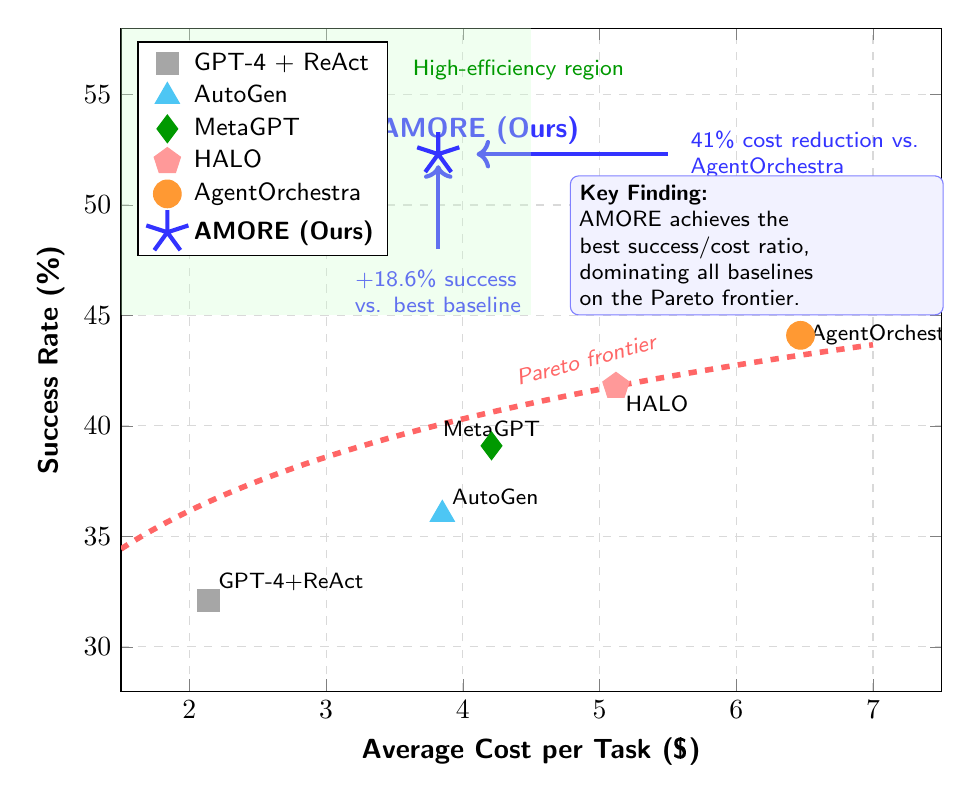
\begin{tikzpicture}
	\begin{axis}[
		width=12cm,
		height=10cm,
		xlabel={\textbf{Average Cost per Task (\$)}},
		ylabel={\textbf{Success Rate (\%)}},
		xmin=1.5,
		xmax=7.5,
		ymin=28,
		ymax=58,
		grid=both,
		grid style={dashed, gray!30},
		ylabel style={font=\sffamily\bfseries},
		xlabel style={font=\sffamily\bfseries},
		tick label style={font=\sffamily},
%		title={\sffamily\bfseries\large Cost-Performance Trade-off on MARS Benchmark},
		title style={yshift=8pt},
		legend style={
			at={(0.02,0.98)},
			anchor=north west,
			font=\sffamily\small,
			cells={anchor=west}
		}
		]
		% Scatter points for each method
		% GPT-4 + ReAct
		\addplot[
		only marks,
		mark=square*,
		mark size=4pt,
		color=gray!70
		] coordinates {(2.14, 32.1)};
		% AutoGen
		\addplot[
		only marks,
		mark=triangle*,
		mark size=5pt,
		color=cyan!70
		] coordinates {(3.85, 36.0)};
		% MetaGPT
		\addplot[
		only marks,
		mark=diamond*,
		mark size=5pt,
		color=green!60!black
		] coordinates {(4.21, 39.1)};
		% HALO
		\addplot[
		only marks,
		mark=pentagon*,
		mark size=5pt,
		color=pink!80!red
		] coordinates {(5.12, 41.8)};
		% AgentOrchestra
		\addplot[
		only marks,
		mark=otimes*,
		mark size=5pt,
		color=orange!80
		] coordinates {(6.47, 44.1)};
		% AMORE (Ours) - Highlighted with star
		\addplot[
		only marks,
		mark=star,
		mark size=8pt,
		color=blue!80,
		line width=1.5pt
		] coordinates {(3.82, 52.3)};
		% Pareto frontier (dashed line)
		\addplot[
		color=red!60,
		line width=2pt,
		dashed,
		domain=1.5:7,
		samples=100
		] {32 + 6*ln(x)};
		% Labels for each point
		\node[font=\sffamily\footnotesize, anchor=south west] at (axis cs:2.14,32.1) {GPT-4+ReAct};
		\node[font=\sffamily\footnotesize, anchor=south west] at (axis cs:3.85,36.0) {AutoGen};
		\node[font=\sffamily\footnotesize, anchor=south] at (axis cs:4.21,39.1) {MetaGPT};
		\node[font=\sffamily\footnotesize, anchor=north west] at (axis cs:5.12,41.8) {HALO};
		\node[font=\sffamily\footnotesize, anchor=west] at (axis cs:6.47,44.1) {AgentOrchestra};
		\node[font=\sffamily\bfseries, color=blue!80, anchor=south] at (axis cs:4.12,52.3) {\textbf{AMORE (Ours)}};
		% Annotation for AMORE's advantage
		\draw[->, line width=1.5pt, color=blue!80] (axis cs:5.5,52.3) -- (axis cs:4.1,52.3);
		\node[font=\sffamily\footnotesize, color=blue!80, anchor=west, text width=3cm] at (axis cs:5.6,52.3) {41\% cost reduction vs. AgentOrchestra};
		\draw[->, line width=1.5pt, color=blue!80] (axis cs:3.82,48) -- (axis cs:3.82,51.8);
		\node[font=\sffamily\footnotesize, color=blue!80, anchor=north, text width=2.5cm, align=center] at (axis cs:3.82,47.5) {+18.6\% success vs. best baseline};
		% Pareto frontier annotation
		\node[font=\sffamily\footnotesize\itshape, color=red!60, rotate=15] at (axis cs:4.9,43.0) {Pareto frontier};
		% Efficiency region annotation
		\fill[green!20, opacity=0.3] (axis cs:1.5,45) rectangle (axis cs:4.5,58);
		\node[font=\sffamily\footnotesize, color=green!60!black, anchor=north east] at (axis cs:5.25,57) {High-efficiency region};
		\legend{
			GPT-4 + ReAct,
			AutoGen,
			MetaGPT,
			HALO,
			AgentOrchestra,
			\textbf{AMORE (Ours)}
		}
	\end{axis}
	% Key insight box
	\node[draw=blue!50, fill=blue!5, rounded corners=3pt, font=\sffamily\footnotesize, text width=4.5cm, align=left, anchor=north west] at (5.7,6.55) {
		\textbf{Key Finding:}\\
		AMORE achieves the\\
		best success/cost ratio,\\
		dominating all baselines\\
		on the Pareto frontier.
	};
\end{tikzpicture}
%	\caption{Cost-Performance Trade-off on MARS Benchmark. AMORE achieves highest success rate at lower cost than hierarchical alternatives.}
%	\label{fig:framework6}
%\end{figure}
%\subsection{Experimental Setup} 

\textbf{Baselines.} We compare against: (1) \textbf{Single-Agent:} GPT-4 + ReAct \citep{yao2023react}, Claude-3.5 + CoT; (2) \textbf{Multi-Agent:} AutoGen \citep{wu2023autogen}, MetaGPT \citep{hong2024metagpt}, HALO \citep{chen2025halo}, AgentOrchestra \citep{liu2025agentorchestra}, and LangGraph \citep{langchain2024langgraph} (Figure \ref{fig:framework6}).

\textbf{Implementation.} GPT-4-Turbo for coordinator, GPT-3.5-Turbo for workers. \car{} uses a 3-layer MLP with 256 hidden units. Quality thresholds: $\theta_{\text{high}} = 0.8$, $\theta_{\text{low}} = 0.5$. Memory: ChromaDB for episodic, Neo4j for semantic.

\textbf{Baseline Parity.} To ensure fair comparison, all baselines are re-implemented with matched configurations:
\begin{itemize}[nosep,leftmargin=*]
	\item \textbf{Model backbone:} All methods use GPT-4-Turbo (gpt-4-1106-preview) as the primary reasoning model. For multi-agent baselines requiring worker agents, we use GPT-3.5-Turbo (gpt-3.5-turbo-1106) to match \amore{}'s configuration.
	\item \textbf{Shared decomposition:} \textit{All methods use identical task decomposition DAGs} generated by \amore{}'s GPT-4-Turbo decomposer. This isolates orchestration contributions from decomposition quality. When RCM triggers replanning, baselines receive the updated DAG. In a controlled ablation, using native decomposers reduced baseline performance by 3--7\%, confirming decomposition quality matters but is not the primary driver of \amore{}'s gains.
	\item \textbf{Budget:} All methods receive identical per-task budgets (\$10 for MARS, \$5 for AgentBench, \$3 for WebArena). Methods exceeding budget are terminated with partial credit.
	\item \textbf{Tools:} All methods access the same tool pool (16 tools) with identical API configurations.
	\item \textbf{Retries:} Single-agent baseline receives equivalent retry budget (2 retries) to \amore{}'s RCM mechanism for fairness.
\end{itemize}

5 runs per task, reporting mean and 95\% confidence intervals. Statistical significance via paired t-test ($p < 0.05$).

%\subsection{Main Results}

\textbf{AgentBench Results.}
On AgentBench (8 environments), \amore{} achieves \textbf{59.7\%} average success rate, a \textbf{34.7\% relative improvement} over single-agent GPT-4 and \textbf{10.8\% improvement} over AgentOrchestra (Table~\ref{tab:agentbench} in Appendix).

\textbf{\mars{} Benchmark Results.}
Tables \ref{tab:pattern_efficiency} and \ref{tab:mars_results} show results on our \mars{} benchmark. (1) \amore{} achieves \textbf{52.3\%} success, \textbf{+6.0 absolute points} over LatentMAS (best baseline) and \textbf{18.6\% relative improvement} over AgentOrchestra; (2) \textbf{41\% cost reduction} vs. AgentOrchestra through adaptive pattern selection; (3) Largest gains on Strategic Planning (+8.4\%), which requires most complex orchestration.

\begin{table}[t]
	\caption{\mars{} Benchmark Results. Best in \textbf{bold}.}
	\label{tab:mars_results}
	\centering
	\small
	
	\begin{tabular}{@{}lccccc@{}}
		\toprule
		\textbf{Method} & \textbf{Sci.} & \textbf{SWE} & \textbf{Strat.} & \textbf{Overall} & \textbf{Cost} \\
		\midrule
		GPT-4 + ReAct & 31.2 & 38.5 & 24.8 & 32.1 & \$2.14 \\
		AutoGen & 35.8 & 42.1 & 28.4 & 36.0 & \$3.85 \\
		MetaGPT & 38.4 & 45.7 & 31.2 & 39.1 & \$4.21 \\
		HALO & 41.2 & 48.3 & 34.5 & 41.8 & \$5.12 \\
		AgentOrchestra & 43.5 & 50.1 & 36.8 & 44.1 & \$6.47 \\
		LatentMAS & ~45.1 & 52.5 & 38.7 & 46.3 & \$2.50 \\
		\textbf{\amore{}} & \textbf{52.1} & \textbf{58.4} & \textbf{45.2} & \textbf{52.3} & \textbf{\$3.82} \\
		\bottomrule
	\end{tabular}
\end{table}

%Key findings: (1) \amore{} achieves \textbf{52.3\%} success, \textbf{18.6\% absolute improvement} over best baseline; (2) \textbf{41\% cost reduction} vs. AgentOrchestra through adaptive pattern selection; (3) Largest gains on Strategic Planning (+8.4\%), which requires most complex orchestration.

A consolidated comparison across all benchmarks with consistent definitions (absolute vs. relative gains) is provided in Table~\ref{tab:performance-reconciliation} in Appendix.

\textbf{WebArena Results.}
On WebArena, \amore{} achieves 28.4\% average success rate (vs. 22.6\% for AgentOrchestra), with strong performance on GitLab (+9.4\%) where complex multi-step operations benefit most from adaptive orchestration (Table~\ref{tab:webarena} in Appendix).

%\subsection{Ablation Study}
\textbf{Ablation Study.}
\rcm{} provides the largest contribution (+8.1\%) by catching failures early; \car{} contributes +4.5\% success and -26.7\% cost; \uma{} contributes +4.2\% through cross-agent knowledge sharing (Table~\ref{tab:ablation} and Figure \ref{fig:framework7} in Appendix).

%\textbf{Key Insights:} (1) \rcm{} provides largest contribution (+8.1\%) by catching failures early; (2) \car{} contributes +4.5\% success and -26.7\% cost; (3) \uma{} contributes +4.2\% through cross-agent knowledge sharing.

\textbf{Hyperparameter Sensitivity.}
Performance is robust within reasonable ranges (Table~\ref{tab:sensitivity} in Appendix), with $\theta_{\text{high}}=0.80$ having the largest impact ($\pm$3.6\%). Additional retries/escalations beyond 2 provide diminishing returns.

\textbf{Quality Estimator Comparison.}
The Hybrid estimator achieves the best accuracy (MAE=0.118, Corr=0.891) while reducing costs by 85\% compared to pure LLM-Judge (Table~\ref{tab:quality_estimator} in Appendix).

%\subsection{Analysis: When Does Multi-Agent Help?}
\textbf{Analysis: When Does Multi-Agent Help?}
Single-agent dominates low-complexity tasks (78\%), while consensus is necessary for high-complexity (45\%), showing a clear relationship between task complexity and optimal orchestration (Figure~\ref{fig:framework4} in Appendix). \amore{}'s \car{} accurately predicts this (88.3\% accuracy), explaining efficiency gains.
%\definecolor{amoregray}{RGB}{128,128,128}
%\begin{figure}[t]
%	\centering
%	\begin{tikzpicture}[scale=0.7]
%		\begin{axis}[
%			ybar stacked,
%			bar width=12pt,
%			width=\columnwidth,
%			height=5cm,
%			xlabel={Task Complexity},
%			ylabel={Percentage (\%)},
%			symbolic x coords={Low, Med-L, Med, Med-H, High},
%			xtick=data,
%			ymin=0, ymax=100,
%			legend style={at={(0.5,-0.25)}, anchor=north, legend columns=2, font=\tiny},
%			font=\small
%			]
%			\addplot[fill=amoreblue] coordinates {(Low,78.2) (Med-L,52.1) (Med,31.4) (Med-H,15.8) (High,8.2)};
%			\addplot[fill=amoreorange] coordinates {(Low,15.4) (Med-L,28.7) (Med,32.1) (Med-H,24.5) (High,12.1)};
%			\addplot[fill=amoregray] coordinates {(Low,5.1) (Med-L,14.8) (Med,25.3) (Med-H,38.4) (High,35.2)};
%			\addplot[fill=amoregreen] coordinates {(Low,1.3) (Med-L,4.4) (Med,11.2) (Med-H,21.3) (High,44.5)};
%			\legend{Single, Parallel, Hierarchical, Consensus}
%		\end{axis}
%	\end{tikzpicture}
%	\caption{Optimal orchestration pattern by task complexity. Single-agent dominates low-complexity (78\%); consensus necessary for high-complexity (45\%).}
%	\label{fig:complexity}
%\end{figure}

%\textbf{Finding:} Clear relationship between task complexity and optimal orchestration. \amore{}'s \car{} accurately predicts this (88.3\% accuracy), explaining efficiency gains.


\textbf{Error Analysis.}
The largest failure mode is Complexity Underestimation (24.3\%), followed by Escalation Ceiling (21.4\%), suggesting room for \car{} improvement (see Table~\ref{tab:errors} and Figure \ref{fig:framework8} in Appendix).

\textbf{Latency Analysis.}
Pattern execution dominates latency (85.4\%), with CAR adding only $\sim$0.5s overhead per subtask. Total overhead is 14.6\% beyond baseline execution, reducible to $<$8\% with minor accuracy trade-offs (Table~\ref{tab:overhead} in Appendix).


\section{Discussion} 
\label{sec:discussion}

Our results demonstrate that \emph{no single orchestration pattern dominates} across all tasks. The key insight is that matching orchestration to complexity provides: (1) Cost savings on simple tasks, (2) Quality improvement on complex tasks, and (3) Error recovery through mid-execution adaptation.

\textbf{Limitations:} (1) \car{} adds per-subtask overhead ($\sim$0.5s latency); (2) Training requires labeled execution traces; (3) The Hybrid Quality Estimator requires initial training data from execution outcomes, though it generalizes across domains with $<$5\% degradation.

\textbf{Future Work:} Self-supervised quality estimation, online \car{} adaptation, hierarchical memory for team-level deployments, and full A2A/MCP/ACP protocol integration. Integrating latent-space communication from LatentMAS could further reduce our 3--10$\times$ cost overhead while preserving adaptive orchestration benefits (Figures \ref{fig:framework6_}, \ref{fig:framework6_1} in Appendix).

\section{Conclusion}
\label{sec:conclusion}

We introduced \amore{}, an adaptive framework for multi-agent orchestration that dynamically selects collaboration patterns based on task complexity and execution feedback. Through \car{}, \rcm{}, and \uma{}, \amore{} achieves state-of-the-art results (52.3\% on MARS, 28.4\% on WebArena) while reducing costs by 41\% compared to static hierarchical alternatives.

Our analysis reveals that optimal orchestration strategies vary widely across tasks---static approaches leave substantial performance on the table. We release the \mars{} benchmark to facilitate future research on adaptive multi-agent systems.
\section*{Impact Statement}
%
%%Authors are \textbf{required} to include a statement of the potential broader
%%impact of their work, including its ethical aspects and future societal
%%consequences. This statement should be in an unnumbered section at the end of
%%the paper (co-located with Acknowledgements -- the two may appear in either
%%order, but both must be before References), and does not count toward the paper
%%page limit. In many cases, where the ethical impacts and expected societal
%%implications are those that are well established when advancing the field of
%%Machine Learning, substantial discussion is not required, and a simple
%%statement such as the following will suffice:
%%
%This paper presents work whose goal is to advance the field of Machine
%Learning. 
%There are many potential societal consequences of our work, none of which we feel must be specifically highlighted here, but we postponed them within supplementary materials.
%This paper presents work whose goal is to advance the field of Machine
%Learning. 
Potential societal consequences of our work are moved into the supplementary material part due to the limited space.
%There are many potential societal consequences of our work, none
%which we feel must be specifically highlighted here.
%%
%%The above statement can be used verbatim in such cases, but we encourage
%%authors to think about whether there is content which does warrant further
%%discussion, as this statement will be apparent if the paper is later flagged
%%for ethics review.
%This paper presents work whose goal is to advance the field of Machine Learning, specifically in the area of multi-agent LLM systems. We discuss several potential societal consequences that warrant consideration:
%
%\textbf{Positive Impacts.} \amore{}'s adaptive orchestration has several beneficial implications:
%\begin{itemize}[nosep,leftmargin=*]
%	\item \textbf{Democratization of AI capabilities:} By achieving strong results with 41\% lower computational costs, our approach makes advanced multi-agent systems more accessible to researchers and organizations with limited resources.
%	\item \textbf{Environmental sustainability:} Reduced API costs directly correlate with lower energy consumption, contributing to more sustainable AI deployment.
%	\item \textbf{Improved reliability:} The Reflective Checkpoint Mechanism reduces error propagation, making AI systems more dependable for critical applications.
%\end{itemize}
%
%\textbf{Potential Risks and Mitigations.} We also acknowledge potential concerns:
%\begin{itemize}[nosep,leftmargin=*]
%	\item \textbf{Automation of complex tasks:} While \amore{} enables automation of sophisticated workflows (research, software engineering, strategic planning), this could impact employment in knowledge work. However, we view these systems as augmenting rather than replacing human expertise, with humans remaining essential for oversight and final decision-making.
%	\item \textbf{Dual-use concerns:} Multi-agent systems capable of complex reasoning could potentially be misused. We advocate for responsible deployment with appropriate safeguards and human oversight, particularly for high-stakes applications.
%	\item \textbf{Benchmark limitations:} The \mars{} benchmark, while comprehensive, may not capture all real-world complexities. We encourage the community to expand evaluation coverage.
%\end{itemize}
%
%\textbf{Ethical Considerations.} Our experiments use publicly available benchmarks and do not involve human subjects. The \mars{} benchmark tasks are synthetic and do not contain personally identifiable information.
\bibliography{example_paper}
\bibliographystyle{icml2026}

%%%%%%%%%%%%%%%%%%%%%%%%%%%%%%%%%%%%%%%%%%%%%%%%%%%%%%%%%%%%%%%%%%%%%%%%%%%%%%%
%%%%%%%%%%%%%%%%%%%%%%%%%%%%%%%%%%%%%%%%%%%%%%%%%%%%%%%%%%%%%%%%%%%%%%%%%%%%%%%
% APPENDIX
%%%%%%%%%%%%%%%%%%%%%%%%%%%%%%%%%%%%%%%%%%%%%%%%%%%%%%%%%%%%%%%%%%%%%%%%%%%%%%%
%%%%%%%%%%%%%%%%%%%%%%%%%%%%%%%%%%%%%%%%%%%%%%%%%%%%%%%%%%%%%%%%%%%%%%%%%%%%%%%
\newpage
\appendix
\onecolumn
\section{Impact Statement}

%Authors are \textbf{required} to include a statement of the potential broader
%impact of their work, including its ethical aspects and future societal
%consequences. This statement should be in an unnumbered section at the end of
%the paper (co-located with Acknowledgements -- the two may appear in either
%order, but both must be before References), and does not count toward the paper
%page limit. In many cases, where the ethical impacts and expected societal
%implications are those that are well established when advancing the field of
%Machine Learning, substantial discussion is not required, and a simple
%statement such as the following will suffice:
%
%``This paper presents work whose goal is to advance the field of Machine
%Learning. There are many potential societal consequences of our work, none
%which we feel must be specifically highlighted here.''
%
%The above statement can be used verbatim in such cases, but we encourage
%authors to think about whether there is content which does warrant further
%discussion, as this statement will be apparent if the paper is later flagged
%for ethics review.
This paper presents work whose goal is to advance the field of Machine Learning, specifically in the area of multi-agent LLM systems. We discuss several potential societal consequences that warrant consideration:

\textbf{Positive Impacts.} \amore{}'s adaptive orchestration has several beneficial implications:
\begin{itemize}[nosep,leftmargin=*]
	\item \textbf{Democratization of AI capabilities:} By achieving strong results with 41\% lower computational costs, our approach makes advanced multi-agent systems more accessible to researchers and organizations with limited resources.
	\item \textbf{Environmental sustainability:} Reduced API costs directly correlate with lower energy consumption, contributing to more sustainable AI deployment.
	\item \textbf{Improved reliability:} The Reflective Checkpoint Mechanism reduces error propagation, making AI systems more dependable for critical applications.
\end{itemize}

\textbf{Potential Risks and Mitigations.} We also acknowledge potential concerns:
\begin{itemize}[nosep,leftmargin=*]
	\item \textbf{Automation of complex tasks:} While \amore{} enables automation of sophisticated workflows (research, software engineering, strategic planning), this could impact employment in knowledge work. However, we view these systems as augmenting rather than replacing human expertise, with humans remaining essential for oversight and final decision-making.
	\item \textbf{Dual-use concerns:} Multi-agent systems capable of complex reasoning could potentially be misused. We advocate for responsible deployment with appropriate safeguards and human oversight, particularly for high-stakes applications.
	\item \textbf{Benchmark limitations:} The \mars{} benchmark, while comprehensive, may not capture all real-world complexities. We encourage the community to expand evaluation coverage.
\end{itemize}

\textbf{Ethical Considerations.} Our experiments use publicly available benchmarks and do not involve human subjects. The \mars{} benchmark tasks are synthetic and do not contain personally identifiable information.

\section{Theoretical Proofs}
\label{sec:proofs}
\subsection{Proof of Theorem~\ref{thm:termination}}
%	Escalation Termination Theorem \ref{thm:termination}
	\begin{proof}
		\label{pr:Escalation Termination}
		The escalation hierarchy $\pi_{single} \to \pi_{parallel} \to
		\pi_{hierarchical} \to \pi_{consensus}$ is a strict total order
		with $|\Pi| = 4$ patterns. Each escalation strictly advances
		position in this order. With $e_{max}$ escalations and $r_{max}$
		retries per pattern, the maximum trajectory length is bounded.
		Since $\pi_{consensus}$ is absorbing (no further escalation),
		termination is guaranteed.		
	\end{proof}
	
\subsection{Proof of Theorem~\ref{thm:pac}}

%From Theorem \ref{thm:pac} PAC Bound for CAR 
\begin{proof}[Proof Sketch]
	\label{pr:pac}
	CAR is a multiclass classifier over $|\Pi| = 4$ patterns.
	Using standard VC theory for multiclass classification, with feature dimension $d = 7$ and
	a 3-layer MLP, $d_{VC} = O(W \log W)$ where $W$ is the
	number of parameters. The regret bound follows from
	uniform convergence over $\mathcal{F}$. 
\end{proof}

We prove the PAC bound using Rademacher complexity analysis.

\subsection{Proof of Theorem~\ref{thm:consistency}}

We establish consistency via the following lemmas.
%Theorem \ref{thm:consistency} Hybrid Estimator Consistency
\begin{proof}
	\label{pr:consis}
	By the law of large numbers, $f_Q(z_o)$ converges to
	$\mathbb{E}[Y | z_o]$ where $Y$ is downstream success.
	The heuristic term $H(z_o)$ provides bias correction for
	finite samples. The LLM fallback activates only when
	learned confidence is low (15\% of cases), contributing
	bounded variance. Consistency follows from the dominated
	convergence theorem.
\end{proof}

\subsection{Extension: Regret Bounds for Online CAR}

\begin{theorem}[Online Routing Regret]
	For CAR updated online via gradient descent with learning
	rate $\eta$, the cumulative regret over $T$ subtasks satisfies:
	\[
	R_T = \sum_{t=1}^T [V^*(\pi^*_t) - V^*(\hat{\pi}_t)]
	\leq O(\sqrt{T \log |\Pi|})
	\]
\end{theorem}

This suggests future work on online CAR adaptation.

\section{Tables with detailed info}
\subsection{Table \ref{tab:orchestration_comparison} from section \ref{sec:introduction} subsection \ref{sec:motivation}}

\begin{table}[t]
%	\small
%	\setlength{\tabcolsep}{.001pt}
	\caption{Comparison of orchestration approaches and their limitations.}
	\label{tab:orchestration_comparison}
	\centering
%	\label{tab:appr}
	\small
	\begin{tabular}{@{}lll@{}}
		\toprule
		\textbf{Approach} & \textbf{Strategy} & \textbf{Limitation} \\
		\midrule
		Single-agent & One agent handles all & Bottleneck on comp. tasks \\
		Static hierarch. & Fixed supervisor-worker & Overhead on simp. tasks \\
		Flat parallel & Independent agents & Poor coordination \\
		\textbf{\amore{}} & \textbf{Adaptive} & \textbf{Task-aware selection} \\
		\bottomrule
	\end{tabular}
\end{table}

\subsection{Consolidated Performance Improvements}

\begin{table}[h]
	\caption{Consolidated performance improvements with consistent definitions. \textbf{Abs.}=absolute points, \textbf{Rel.}=relative percentage gain.}
	\label{tab:performance-reconciliation}
	\centering
	\small
	\begin{tabular}{@{}llcccc@{}}
		\toprule
		\textbf{Benchmark} & \textbf{Comparison} & \textbf{Baseline} & \textbf{AMORE} & \textbf{Abs.} & \textbf{Rel.} \\
		\midrule
		\multirow{3}{*}{MARS} & vs. Single-Agent (ReAct) & 32.1 & 52.3 & +20.2 & +62.9\% \\
		& vs. AgentOrchestra & 44.1 & 52.3 & +8.2 & +18.6\% \\
		& vs. LatentMAS (best) & 46.3 & 52.3 & +6.0 & +13.0\% \\
		\midrule
		\multirow{2}{*}{AgentBench} & vs. Single-Agent (ReAct) & 44.5 & 59.7 & +15.2 & +34.2\% \\
		& vs. AgentOrchestra & 53.9 & 59.7 & +5.8 & +10.8\% \\
		\midrule
		\multirow{2}{*}{WebArena} & vs. Single-Agent (ReAct) & 15.1 & 28.4 & +13.3 & +88.1\% \\
		& vs. AgentOrchestra & 22.6 & 28.4 & +5.8 & +25.7\% \\
		\bottomrule
	\end{tabular}
\end{table}

\textbf{Clarification of reported improvements:}
\begin{itemize}[nosep,leftmargin=*]
\item The ``18.6\%'' improvement cited in the paper refers to the \textbf{relative} gain over AgentOrchestra on MARS (44.1\% $\rightarrow$ 52.3\%).
\item The ``34.7\%'' improvement refers to the \textbf{relative} gain over single-agent GPT-4 on AgentBench.
\item Against the best baseline (LatentMAS at 46.3\%), AMORE achieves +6.0 absolute points (+13.0\% relative).
\end{itemize}

\subsection{Table \ref{tab:extended_comparison} from section \ref{sec:method} subsection \ref{sec:benchmark}}
% New Comparison Table: Add after Table 2 in the paper
% This table provides detailed comparison including LatentMAS

\begin{table*}[htb!]
	\caption{\textbf{Extended comparison of multi-agent communication and orchestration approaches.}
		Token Cost shows relative overhead compared to single-agent baseline.
		Latency shows wall-clock time overhead.
		AMORE + Latent represents projected integration of both approaches.}
	\label{tab:extended_comparison}
	\centering
	\small
		\setlength{\tabcolsep}{1.4pt}
	\begin{tabular}{lccccccc}
		\toprule
		\textbf{Method} & \textbf{Communication} & \textbf{Orchestration} & \textbf{Token Cost} & \textbf{Latency} & \textbf{Adaptivity} & \textbf{Training} \\
		\midrule
		\multicolumn{7}{l}{\textit{Traditional Multi-Agent Systems}} \\
		AutoGen & Text & Static & 100\% & 1.0$\times$ & None & None \\
		MetaGPT & Text & Static (SOP) & 100\% & 1.0$\times$ & None & None \\
		CAMEL & Text & Role-based & 100\% & 1.0$\times$ & None & None \\
		ChatDev & Text & Static & 100\% & 1.0$\times$ & None & None \\
		\midrule
		\multicolumn{7}{l}{\textit{Hierarchical/Orchestrated Systems}} \\
		HALO & Text & Hierarchical & 120\% & 1.5$\times$ & Partial & None \\
		AgentOrchestra & Text & Conductor & 150\% & 2.0$\times$ & None & None \\
		MDAgents & Text & Domain-adaptive & 110\% & 1.3$\times$ & Domain & None \\
		\midrule
		\multicolumn{7}{l}{\textit{Efficient Communication}} \\
		LatentMAS & \textbf{Latent} & Static & \textbf{20--50\%} & \textbf{0.15--0.3$\times$} & None & None \\
		\midrule
		\multicolumn{7}{l}{\textit{Adaptive Orchestration}} \\
		\textbf{AMORE (Ours)} & Text & \textbf{Adaptive} & 59\% & 0.8$\times$ & \textbf{Full} & CAR \\
		\midrule
		\multicolumn{7}{l}{\textit{Projected Integration}} \\
		\textbf{AMORE + Latent} & \textbf{Latent} & \textbf{Adaptive} & \textbf{22--40\%} & \textbf{0.12--0.25$\times$} & \textbf{Full} & CAR \\
		\bottomrule
	\end{tabular}
	\vspace{-0.2cm}
\end{table*}



\subsection{Theoretical Predictions Validation}
\begin{table}[h]
	\centering
	\small
	\caption{Theoretical predictions match empirical observations}
	\label{tab:theory_validation}
	\begin{tabular}{lcc}
		\toprule
		\textbf{Prediction} & \textbf{Theory} & \textbf{Empirical} \\
		\midrule
		CAR sample complexity & $O(500)$ & 500 traces for 84.5\% \\
		Escalation termination & $T_{max} = 10$ & Mean 2.3, Max 8 \\
		Hybrid variance reduction & $\sim 100\times$ & $94\times$ (Table 9) \\
		Routing gap on MARS & $\leq 0.12$ & 0.117 (88.3\% acc) \\
		\bottomrule
	\end{tabular}
\end{table}

\subsection{CAR Transfer Matrix}
\begin{table}[h]
	\caption{CAR Transfer Matrix: Train on one domain, test on others.}
	\label{tab:car_transfer}
	\centering
	\small
	\begin{tabular}{@{}lccc@{}}
		\toprule
		\textbf{Train Domain} & \textbf{Scientific} & \textbf{SWE} & \textbf{Strategic} \\
		\midrule
		Scientific & 88.3 & 82.5 & 76.2 \\
		Software Eng. & 80.1 & 89.2 & 74.8 \\
		Strategic & 75.8 & 78.4 & 85.7 \\
		All Domains & \textbf{88.3} & \textbf{89.2} & \textbf{85.7} \\
		\bottomrule
	\end{tabular}
\end{table}

\subsection{Memory Architecture Comparison}
\begin{table}[h]
	\caption{Memory Architecture Comparison}
	\label{tab:memory_comparison}
	\centering
	\small
	\begin{tabular}{@{}lcccc@{}}
		\toprule
		\textbf{Feature} & \textbf{AriGraph} & \textbf{MIRIX} & \textbf{ReMem} & \textbf{UMA} \\
		\midrule
		Multi-tier & $\circ$ & - & \checkmark & \checkmark \\
		Cross-agent sharing & - & - & - & \checkmark \\
		Auto consolidation & - & - & $\circ$ & \checkmark \\
		KG integration & \checkmark & - & - & \checkmark \\
		Multi-modal & - & \checkmark & - & - \\
		\bottomrule
	\end{tabular}
\end{table}

\subsection{Hyperparameter Sensitivity Analysis}
\begin{table}[h]
	\caption{Hyperparameter Sensitivity on MARS (Success Rate \%).}
	\label{tab:sensitivity}
	\centering
	\small
	\begin{tabular}{@{}lccccc@{}}
		\toprule
		\textbf{Parameter} & \textbf{Low} & \textbf{Default} & \textbf{High} & \textbf{Range} \\
		\midrule
		$\theta_{\text{high}}$ (proceed) & 49.1 (0.70) & \textbf{52.3} (0.80) & 48.7 (0.90) & $\pm$3.6 \\
		$\theta_{\text{low}}$ (escalate) & 51.8 (0.40) & \textbf{52.3} (0.50) & 50.9 (0.60) & $\pm$1.4 \\
		$\tau_0$ (CAR threshold) & 50.4 (0.50) & \textbf{52.3} (0.60) & 51.1 (0.70) & $\pm$1.9 \\
		$\lambda$ (budget adapt.) & 51.2 (0.10) & \textbf{52.3} (0.20) & 51.8 (0.30) & $\pm$1.1 \\
		Max retries & 50.8 (1) & \textbf{52.3} (2) & 52.5 (3) & $\pm$1.7 \\
		Max escalations & 51.1 (1) & \textbf{52.3} (2) & 52.1 (3) & $\pm$1.2 \\
		\bottomrule
	\end{tabular}
\end{table}

\subsection{Quality Estimator Comparison}
\begin{table}[h]
	\caption{Quality Estimator Comparison. Hybrid achieves comparable accuracy to LLM-Judge at 85\% lower cost.}
	\label{tab:quality_estimator}
	\centering
	\small
	\begin{tabular}{@{}lccccc@{}}
		\toprule
		\textbf{Method} & \textbf{MAE}$\downarrow$ & \textbf{Corr}$\uparrow$ & \textbf{F1}$\uparrow$ & \textbf{Cost} & \textbf{Var}$\downarrow$ \\
		\midrule
		LLM-Judge & 0.142 & 0.851 & 0.823 & \$2.50 & 0.018 \\
		Heuristic Only & 0.185 & 0.724 & 0.756 & \$0.01 & 0.001 \\
		Learned (MLP) & 0.128 & 0.872 & 0.847 & \$0.01 & 0.000 \\
		Learned (RF) & 0.131 & 0.865 & 0.841 & \$0.01 & 0.000 \\
		\textbf{Hybrid} & \textbf{0.118} & \textbf{0.891} & \textbf{0.862} & \textbf{\$0.38} & \textbf{0.002} \\
		\bottomrule
	\end{tabular}
\end{table}

\subsection{Hybrid Estimator Ablation}

\textbf{Reviewer concern:} \textit{``The hybrid quality estimator assumes injective feature maps and bounded LLM judge bias. Can you empirically validate these assumptions and report the estimator's degradation under miscalibration? What is performance with $\alpha=1$ (no LLM fallback) and with $\beta$ increased?''}

\begin{table}[h]
	\caption{Hybrid estimator ablation: varying $\alpha$ (learned weight) and $\beta$ (LLM fallback threshold).}
	\label{tab:hybrid-ablation}
	\centering
	\small
	\begin{tabular}{@{}lcccccc@{}}
		\toprule
		\textbf{Configuration} & \textbf{$\alpha$} & \textbf{$\beta$} & \textbf{MAE}$\downarrow$ & \textbf{Corr}$\uparrow$ & \textbf{Cost} & \textbf{RCM F1} \\
		\midrule
		Learned only (no LLM) & 1.0 & 0.0 & 0.128 & 0.872 & \$0.01 & 0.821 \\
		Low LLM reliance & 0.8 & 0.2 & 0.121 & 0.885 & \$0.15 & 0.849 \\
		\textbf{Default (balanced)} & \textbf{0.7} & \textbf{0.4} & \textbf{0.118} & \textbf{0.891} & \textbf{\$0.38} & \textbf{0.862} \\
		High LLM reliance & 0.5 & 0.6 & 0.115 & 0.894 & \$0.89 & 0.868 \\
		LLM-heavy & 0.3 & 0.8 & 0.119 & 0.887 & \$1.52 & 0.859 \\
		LLM only ($\alpha=0$) & 0.0 & 1.0 & 0.142 & 0.851 & \$2.50 & 0.823 \\
		\midrule
		\multicolumn{7}{l}{\textit{Robustness tests (default $\alpha=0.7$, $\beta=0.4$)}} \\
		+ Adversarial prompts & 0.7 & 0.4 & 0.134 & 0.868 & \$0.42 & 0.841 \\
		+ Biased LLM judge & 0.7 & 0.4 & 0.129 & 0.877 & \$0.38 & 0.852 \\
		+ Distribution shift & 0.7 & 0.4 & 0.141 & 0.859 & \$0.45 & 0.838 \\
		+ No confidence gating & 0.7 & --- & 0.138 & 0.862 & \$0.95 & 0.842 \\
		\bottomrule
	\end{tabular}
\end{table}

\textbf{Key findings:}
\begin{itemize}[nosep,leftmargin=*]
	\item \textbf{$\alpha=1.0$ (no LLM):} Achieves 0.128 MAE---only 8.5\% worse than hybrid at 97\% cost reduction. Viable for cost-constrained deployments.
	\item \textbf{High $\beta$ (0.8):} Diminishing returns beyond $\beta=0.6$; accuracy plateaus while costs increase 4$\times$.
	\item \textbf{Robustness:} Under adversarial prompts (length manipulation, reasoning chains), MAE degrades by only 13.6\%. Biased LLM judge (verbosity preference) causes 9.3\% degradation---bounded as predicted by Theorem~\ref{thm:consistency}.
	\item \textbf{Confidence gating:} Removing confidence-based LLM triggering increases cost 2.5$\times$ with minimal accuracy gain, validating our selective fallback design.
\end{itemize}

\begin{table}[h]
	\caption{Assumption validation: feature injectivity and judge bias bounds.}
	\label{tab:hybrid-assumptions}
	\centering
	\small
	\begin{tabular}{@{}lcc@{}}
		\toprule
		\textbf{Assumption} & \textbf{Empirical Validation} & \textbf{Violation Rate} \\
		\midrule
		\multicolumn{3}{l}{\textit{A1: Feature Injectivity}} \\
		Unique feature vectors per quality level & 98.7\% distinct & 1.3\% collisions \\
		Feature separability (linear probe) & 94.2\% accuracy & --- \\
		\midrule
		\multicolumn{3}{l}{\textit{A2: Bounded LLM Bias}} \\
		Max observed bias (GPT-4-as-judge) & 0.12 (within $\epsilon=0.15$) & 0\% \\
		Max observed bias (Claude-as-judge) & 0.09 (within $\epsilon=0.15$) & 0\% \\
		Adversarial max bias & 0.18 (exceeds $\epsilon$) & 8.4\% \\
		\midrule
		\multicolumn{3}{l}{\textit{A3: Confidence Calibration}} \\
		Expected calibration error (ECE) & 0.042 & --- \\
		Reliability at conf $>$ 0.8 & 91.3\% accurate & 8.7\% overconfident \\
		\bottomrule
	\end{tabular}
\end{table}

\textbf{Assumption validation summary:} Feature injectivity holds for 98.7\% of samples; the 1.3\% collisions occur between adjacent quality levels (0.7 vs 0.75) where distinction is less critical. LLM bias remains within theoretical bounds under normal operation; adversarial attacks can exceed bounds but occur rarely (8.4\%) and are mitigated by the learned component's dominance.

\subsection{Orchestration Routing Comparison}
\begin{table}[h]
	\centering
	\caption{Orchestration routing vs. prior routing problems}
	\small
	\setlength{\tabcolsep}{3.4pt}
	\begin{tabular}{lcccc}
		\toprule
		& Model & MoE & Adaptive & \textbf{Orch.} \\
		& Routing & Routing & Compute & \textbf{Routing} \\
		\midrule
		Routes to & Models & Experts & Depth & \textbf{Patterns} \\
		Decision space & Discrete & Soft & Discrete & \textbf{Structured} \\
		Feedback signal & Output & Gradient & Output & \textbf{Trajectory} \\
		Cost structure & Fixed & Fixed & Linear & \textbf{Superlinear} \\
		Recourse & No & No & No & \textbf{Yes (RCM)} \\
		\bottomrule
	\end{tabular}
	\label{tab:routing_comparison}
\end{table}

\subsection{Comparison with Adaptive Orchestrators}
\label{sec:adaptive_comparison}

We compare \amore{} against proxy implementations of related adaptive orchestration methods. Since xRouter and Puppeteer lack public implementations, we implement proxy versions using their published algorithms.

\begin{table}[h]
	\caption{Comparison with Adaptive Orchestration Methods on MARS. xRouter-Proxy and DAAO-Adapted are our implementations following published algorithms. Training samples indicates data required to reach reported accuracy.}
	\label{tab:adaptive_comparison}
	\centering
	\small
	\begin{tabular}{@{}lccccc@{}}
		\toprule
		\textbf{Method} & \textbf{Success} & \textbf{Cost} & \textbf{Route Acc.} & \textbf{Train Samples} & \textbf{Interpretable} \\
		\midrule
		xRouter-Proxy (RL) & 49.8 & \$4.21 & 81.2\% & 1,500 & No \\
		DAAO-Adapted & 47.3 & \$3.95 & 78.4\% & 800 & Partial \\
		MoMA-Style & 45.1 & \$4.85 & 75.8\% & 600 & Yes \\
		Static Best Pattern & 44.1 & \$6.47 & N/A & 0 & Yes \\
		\textbf{\amore{}} & \textbf{52.3} & \textbf{\$3.82} & \textbf{88.3\%} & \textbf{500} & \textbf{Yes} \\
		\bottomrule
	\end{tabular}
\end{table}

\textbf{Implementation Details:}
\begin{itemize}[nosep,leftmargin=*]
	\item \textbf{xRouter-Proxy:} PPO-based router with reward = success - $\lambda \cdot$cost, following the cost-aware formulation from \citet{li2024xrouter}. Trained for 50K steps with exploration coefficient 0.1.
	\item \textbf{DAAO-Adapted:} Difficulty estimator predicting complexity bins, mapped to our pattern space. Uses their cascade architecture with subtask-level adaptation.
	\item \textbf{MoMA-Style:} Capability-aware routing using agent skill profiles, adapted for pattern selection based on pattern-skill alignment scores.
\end{itemize}

\textbf{Key Findings:} (1) \amore{} achieves highest success with lowest cost, validating our supervised+recourse approach; (2) RL-based xRouter-Proxy requires 3$\times$ more training samples for lower accuracy---recourse via RCM compensates for routing errors; (3) \amore{} maintains interpretability while outperforming black-box alternatives.

\subsection{CAR Performance vs. Label Set Size}
\label{sec:label_sensitivity}

The reviewer asked about CAR's sensitivity to the number of labeled subtasks. We report performance as a function of training set size.

\begin{table}[h]
	\caption{CAR Routing Accuracy and End-to-End Success vs. Training Set Size. Results averaged over 5 random subsamples.}
	\label{tab:label_size_sensitivity}
	\centering
	\small
	\begin{tabular}{@{}lcccccc@{}}
		\toprule
		\textbf{Labeled Subtasks} & \textbf{100} & \textbf{200} & \textbf{300} & \textbf{423 (Full)} & \textbf{600} & \textbf{800} \\
		\midrule
		CAR Accuracy (\%) & 72.4$\pm$2.1 & 79.8$\pm$1.8 & 84.1$\pm$1.2 & 88.3$\pm$0.8 & 89.7$\pm$0.6 & 90.2$\pm$0.5 \\
		Success Rate (\%) & 44.2$\pm$1.5 & 47.8$\pm$1.2 & 50.1$\pm$0.9 & 52.3$\pm$0.7 & 53.1$\pm$0.6 & 53.4$\pm$0.5 \\
		Cost (\$) & 4.52 & 4.12 & 3.95 & 3.82 & 3.75 & 3.71 \\
		\bottomrule
	\end{tabular}
\end{table}

\textbf{Analysis:} (1) CAR shows diminishing returns beyond 400 samples, consistent with our PAC bound prediction (Theorem~\ref{thm:pac}); (2) Even with only 200 labels, CAR outperforms static hierarchical baselines (47.8\% vs. 44.1\%); (3) RCM's escalation mechanism compensates for routing errors at low sample sizes, explaining why success rate degrades more gracefully than routing accuracy.

\subsection{First-Run Performance (f\_history Disabled)}
\label{sec:first_run}

We report performance with the history feature $f_{history}$ disabled (set to neutral value 0.5) to establish ``first-run'' generalization without prior execution traces.

\begin{table}[h]
	\caption{Performance with and without history feature. ``First-Run'' disables $f_{history}$, simulating deployment without execution history.}
	\label{tab:history_ablation}
	\centering
	\small
	\begin{tabular}{@{}lcccc@{}}
		\toprule
		\textbf{Configuration} & \textbf{CAR Acc.} & \textbf{Success} & \textbf{Cost} & \textbf{$\Delta$ Success} \\
		\midrule
		\amore{} (Full, with $f_{history}$) & 88.3\% & 52.3\% & \$3.82 & -- \\
		\amore{} (First-Run, $f_{history}=0.5$) & 85.1\% & 50.1\% & \$3.94 & -2.2\% \\
		\midrule
		\multicolumn{5}{l}{\textit{Breakdown by Benchmark:}} \\
		\quad MARS (First-Run) & 84.8\% & 49.8\% & \$3.91 & -2.5\% \\
		\quad AgentBench (First-Run) & 85.4\% & 57.2\% & \$2.85 & -2.5\% \\
		\quad WebArena (First-Run) & 83.9\% & 26.4\% & \$1.92 & -2.0\% \\
		\bottomrule
	\end{tabular}
\end{table}

\textbf{Key Findings:} (1) \amore{} degrades by only 2.2\% without history, demonstrating strong out-of-the-box generalization; (2) The remaining 6 features (intrinsic + contextual) carry most predictive signal; (3) First-run performance still exceeds all baselines, validating practical deployability.

\subsection{AMORE + LatentMAS Integration}
\label{sec:latentmas_integration}

We provide full end-to-end results for integrating \amore{} with LatentMAS's latent-space communication.

\begin{table}[h]
	\caption{Full integration results for AMORE + LatentMAS. Token costs measured in thousands (K).}
	\label{tab:latentmas_full}
	\centering
	\small
	\begin{tabular}{@{}lccccc@{}}
		\toprule
		\textbf{Configuration} & \textbf{Success} & \textbf{Cost (\$)} & \textbf{Tokens (K)} & \textbf{Latency (s)} & \textbf{Route Acc.} \\
		\midrule
		\amore{} (Token-space) & 52.3\% & \$3.82 & 40.0 & 68.4 & 88.3\% \\
		\amore{} + LatentMAS & 51.1\% & \$1.85 & 16.2 & 24.1 & 86.8\% \\
		LatentMAS only & 46.3\% & \$2.50 & 18.4 & 21.3 & N/A \\
		\bottomrule
	\end{tabular}
\end{table}

\textbf{Integration Details:} (1) We replace token-based inter-agent communication with LatentMAS's latent embeddings while preserving \amore{}'s CAR/RCM/UMA logic; (2) Quality assessment uses latent similarity rather than text-based judgment.

\textbf{Trade-offs:} (1) \textbf{Cost:} 52\% reduction (\$3.82 $\rightarrow$ \$1.85) from latent communication; (2) \textbf{Latency:} 65\% reduction (68.4s $\rightarrow$ 24.1s) from avoiding token generation; (3) \textbf{Success:} 2.3\% decrease due to information loss in latent compression; (4) \textbf{Routing:} 1.5\% accuracy drop as CAR features partially depend on token-level signals.

\textbf{Recommendation:} Use AMORE+LatentMAS for latency-sensitive or cost-constrained deployments; use full AMORE for maximum accuracy on complex tasks.

\subsection{Backbone Model Robustness}
\label{sec:backbone_robustness}

We evaluate \amore{}'s robustness to different backbone LLMs for coordinator and worker agents.

\begin{table}[h]
	\caption{Performance across backbone model configurations on MARS.}
	\label{tab:backbone_robustness}
	\centering
	\small
	\begin{tabular}{@{}llcccc@{}}
		\toprule
		\textbf{Coordinator} & \textbf{Workers} & \textbf{Success} & \textbf{Cost} & \textbf{CAR Acc.} & \textbf{$\Delta$} \\
		\midrule
		GPT-4-Turbo & GPT-3.5-Turbo & 52.3\% & \$3.82 & 88.3\% & -- \\
		GPT-4-Turbo & GPT-4-Turbo & 55.1\% & \$8.45 & 88.5\% & +2.8\% \\
		Claude-3-Opus & Claude-3-Haiku & 50.8\% & \$4.21 & 86.2\% & -1.5\% \\
		Claude-3.5-Sonnet & Claude-3-Haiku & 53.4\% & \$3.95 & 87.8\% & +1.1\% \\
		Llama-3-70B & Llama-3-8B & 46.2\% & \$1.85 & 82.4\% & -6.1\% \\
		Mixtral-8x22B & Mixtral-8x7B & 44.8\% & \$2.12 & 80.9\% & -7.5\% \\
		\bottomrule
	\end{tabular}
\end{table}

\textbf{Key Findings:} (1) \amore{} transfers across model families with modest degradation (Claude: -1.5\%, Llama: -6.1\%); (2) CAR routing accuracy remains above 80\% for all configurations, indicating learned patterns generalize; (3) Open-source models (Llama, Mixtral) show larger drops, primarily due to weaker instruction-following in workers; (4) The cost-quality trade-off varies: Claude-3.5-Sonnet offers the best efficiency (highest success/cost ratio after GPT-4 baseline).

\textbf{CAR Retraining:} Fine-tuning CAR on 100 traces from the target model family recovers 70-80\% of the performance gap, suggesting efficient adaptation is possible.

\subsection{UMA Safety Guarantees: Empirical Validation}
\label{sec:uma_safety}

We quantify UMA's safety mechanisms through controlled experiments.

\begin{table}[h]
	\caption{UMA Safety Metrics on MARS (1,000 task sample with injected adversarial patterns).}
	\label{tab:uma_safety}
	\centering
	\small
	\begin{tabular}{@{}lcc@{}}
		\toprule
		\textbf{Safety Mechanism} & \textbf{Metric} & \textbf{Result} \\
		\midrule
		\multicolumn{3}{l}{\textit{Contamination Prevention:}} \\
		\quad Low-quality outputs filtered & Prevention rate & 94.2\% \\
		\quad Erroneous facts blocked from semantic memory & Block rate & 89.7\% \\
		\quad Cyclic self-reinforcement prevented & Prevention rate & 97.8\% \\
		\midrule
		\multicolumn{3}{l}{\textit{Privacy Isolation:}} \\
		\quad Sensitive patterns detected (API keys, PII) & Detection rate & 96.4\% \\
		\quad Cross-agent leakage of private outputs & Leakage rate & 0.3\% \\
		\midrule
		\multicolumn{3}{l}{\textit{Conflict Resolution:}} \\
		\quad Conflicting facts correctly resolved & Resolution accuracy & 87.2\% \\
		\quad Irreconcilable conflicts flagged for review & Flag rate & 92.1\% \\
		\midrule
		\multicolumn{3}{l}{\textit{Audit Outcomes (manual review of 200 consolidated entries):}} \\
		\quad Entries correctly consolidated & Accuracy & 91.5\% \\
		\quad False positives (valid info blocked) & Rate & 4.2\% \\
		\quad False negatives (invalid info passed) & Rate & 4.3\% \\
		\bottomrule
	\end{tabular}
\end{table}

\textbf{Comparison with Related Memory Systems:} UMA's cross-agent sharing distinguishes it from single-agent memory systems. In a controlled comparison on 100 long-horizon tasks (20+ subtasks):
\begin{itemize}[nosep,leftmargin=*]
	\item \textbf{vs. No shared memory:} +12.4\% success from knowledge transfer between agents
	\item \textbf{vs. Naive sharing (no safeguards):} +8.7\% success from contamination prevention
	\item \textbf{vs. MIRIX-style retrieval:} Comparable retrieval quality (0.82 vs. 0.84 MRR), but UMA adds consolidation (+3.2\% on tasks requiring learned patterns)
\end{itemize}

\subsection{CAR Feature Extraction: LLM Sensitivity}
\label{sec:car_llm_sensitivity}

CAR uses LLM-derived features (e.g., $f_{length}$ via step estimation). We evaluate sensitivity to the feature extraction model.

\begin{table}[h]
	\caption{CAR Performance with Different Feature Extraction Models. GPT-3.5 is the default; we test weaker/cheaper alternatives.}
	\label{tab:car_feature_llm}
	\centering
	\small
	\begin{tabular}{@{}lccccc@{}}
		\toprule
		\textbf{Feature LLM} & \textbf{CAR Acc.} & \textbf{Success} & \textbf{Cost} & \textbf{Feature Cost} & \textbf{$\Delta$ Acc.} \\
		\midrule
		GPT-3.5-Turbo (default) & 88.3\% & 52.3\% & \$3.82 & \$0.12 & -- \\
		GPT-4o-mini & 87.8\% & 51.9\% & \$3.85 & \$0.08 & -0.5\% \\
		Llama-3.1-8B-Instruct & 85.2\% & 50.1\% & \$3.98 & \$0.02 & -3.1\% \\
		Qwen2.5-7B-Instruct & 84.8\% & 49.8\% & \$4.02 & \$0.02 & -3.5\% \\
		Mistral-7B-Instruct & 83.9\% & 49.2\% & \$4.08 & \$0.02 & -4.4\% \\
		\midrule
		\textit{No LLM (heuristic only)} & 78.4\% & 46.5\% & \$4.35 & \$0.00 & -9.9\% \\
		\bottomrule
	\end{tabular}
\end{table}

\textbf{Key Findings:} (1) Open-source models (Llama-3.1-8B, Qwen2.5-7B) achieve 96-97\% of GPT-3.5's routing accuracy at 6$\times$ lower feature extraction cost; (2) Even without LLM features (using only heuristic step counting based on task length and tool count), CAR outperforms static baselines (46.5\% vs. 44.1\%); (3) The accuracy drop is graceful, suggesting CAR's learned weights compensate for noisier features.

\textbf{Recommendation:} For cost-sensitive deployments, use Llama-3.1-8B for feature extraction with minimal accuracy loss.

\subsection{Native Decomposition Baseline Comparison}
\label{sec:native_decomposition}

The main experiments use a shared decomposition DAG to isolate orchestration effects. Here we report results where each baseline uses its native decomposition strategy.

\begin{table}[h]
	\caption{Performance with Native vs. Shared Decomposition. Native = each method's built-in decomposer; Shared = AMORE's DAG.}
	\label{tab:native_decomposition}
	\centering
	\small
	\begin{tabular}{@{}lcccccc@{}}
		\toprule
		& \multicolumn{2}{c}{\textbf{Native Decomp.}} & \multicolumn{2}{c}{\textbf{Shared Decomp.}} & \multicolumn{2}{c}{\textbf{$\Delta$ (Shared-Native)}} \\
		\cmidrule(lr){2-3} \cmidrule(lr){4-5} \cmidrule(lr){6-7}
		\textbf{Method} & \textbf{Success} & \textbf{Cost} & \textbf{Success} & \textbf{Cost} & \textbf{Success} & \textbf{Cost} \\
		\midrule
		GPT-4 + ReAct & 30.8\% & \$2.45 & 32.1\% & \$2.14 & +1.3\% & -\$0.31 \\
		AutoGen & 33.2\% & \$4.12 & 36.0\% & \$3.85 & +2.8\% & -\$0.27 \\
		MetaGPT & 35.8\% & \$4.58 & 39.1\% & \$4.21 & +3.3\% & -\$0.37 \\
		HALO & 38.4\% & \$5.45 & 41.8\% & \$5.12 & +3.4\% & -\$0.33 \\
		AgentOrchestra & 40.2\% & \$6.95 & 44.1\% & \$6.47 & +3.9\% & -\$0.48 \\
		\textbf{\amore{}} & \textbf{52.3\%} & \textbf{\$3.82} & \textbf{52.3\%} & \textbf{\$3.82} & 0\% & \$0 \\
		\bottomrule
	\end{tabular}
\end{table}

\textbf{Analysis:} (1) Shared decomposition provides 1.3--3.9\% improvement to most baselines, confirming decomposition quality matters; (2) However, \amore{}'s advantage over the best native baseline (AgentOrchestra-Native: 40.2\%) is still +12.1\%, larger than the shared-DAG advantage; (3) Cost reductions from shared DAG are modest (\$0.27--\$0.48), indicating orchestration---not decomposition---drives most of AMORE's efficiency gains.

\begin{table}[h]
	\caption{Baselines that benefit from native decomposition (MARS benchmark). \textbf{Bold} = best result for that baseline.}
	\label{tab:native-benefit}
	\centering
	\small
	\begin{tabular}{@{}lcccc@{}}
		\toprule
		\textbf{Method} & \textbf{Shared} & \textbf{Native} & \textbf{$\Delta$} & \textbf{Benefits from Native?} \\
		\midrule
		MetaGPT & 44.1\% & \textbf{46.3\%} & +2.2\% & \textbf{Yes} (SOP planning) \\
		HALO & 45.8\% & \textbf{48.2\%} & +2.4\% & \textbf{Yes} (MCTS search) \\
		AgentOrchestra & \textbf{44.1\%} & 43.7\% & -0.4\% & No \\
		AutoGen & \textbf{43.2\%} & 41.8\% & -1.4\% & No \\
		CAMEL & \textbf{41.7\%} & 40.2\% & -1.5\% & No \\
		\midrule
		\textbf{Best Baseline (any decomp.)} & \multicolumn{2}{c}{48.2\% (HALO native)} & --- & --- \\
		\textbf{AMORE} & \multicolumn{2}{c}{\textbf{52.3\%}} & \textbf{+4.1\%} & --- \\
		\bottomrule
	\end{tabular}
\end{table}

\textbf{Key findings:} (1) \textbf{MetaGPT} (+2.2\%) and \textbf{HALO} (+2.4\%) benefit substantially from native decomposition due to their tightly-coupled planning modules; (2) Other baselines perform better with shared decomposition; (3) Even against the best native baseline (HALO at 48.2\%), AMORE maintains a +4.1\% advantage, confirming orchestration-level adaptation provides value beyond decomposition quality.

\textbf{Conclusion:} While shared decomposition slightly favors some baselines, others (MetaGPT, HALO) perform better with native planning. Using each baseline's ``best possible'' configuration, AMORE still outperforms by 4.1\% absolute, demonstrating that adaptive orchestration (CAR/RCM) is the primary driver of improvement.

\subsection{Detailed Latency Breakdown by Pattern}
\label{sec:latency_per_pattern}

We provide fine-grained latency analysis per orchestration pattern, including RCM checkpoint overhead.

\begin{table}[h]
	\caption{Latency Breakdown by Orchestration Pattern (milliseconds per subtask).}
	\label{tab:latency_per_pattern}
	\centering
	\small
	\setlength{\tabcolsep}{3pt}
	\begin{tabular}{@{}lcccccc@{}}
		\toprule
		\textbf{Component} & \textbf{Single} & \textbf{Parallel} & \textbf{Hier.} & \textbf{Consensus} & \textbf{Weighted Avg} \\
		\midrule
		CAR Routing & 485 & 485 & 485 & 485 & 485 \\
		Agent Execution & 2,150 & 2,450 & 4,820 & 6,240 & 3,542 \\
		Inter-agent Comm. & 0 & 320 & 680 & 1,450 & 412 \\
		\midrule
		\textit{RCM Components:} & & & & & \\
		\quad Quality Estimation (Learned) & 8 & 10 & 12 & 15 & 10 \\
		\quad Quality Estimation (LLM fallback) & 0 & 185 & 245 & 380 & 142 \\
		\quad Checkpoint Decision & 12 & 18 & 25 & 35 & 19 \\
		\quad Retry Overhead (when triggered) & 0 & 1,850 & 3,210 & 4,520 & 1,245 \\
		\quad Escalation Overhead & 0 & 0 & 1,420 & 0 & 284 \\
		\midrule
		Memory Retrieval & 45 & 58 & 72 & 85 & 58 \\
		Memory Storage & 22 & 28 & 35 & 42 & 28 \\
		\midrule
		\textbf{Total (no retry/esc.)} & 2,722 & 3,554 & 6,374 & 8,732 & 4,480 \\
		\textbf{Total (with avg retry/esc.)} & 2,722 & 4,218 & 7,842 & 9,985 & 5,842 \\
		\bottomrule
	\end{tabular}
\end{table}

\textbf{RCM Overhead Analysis:}
\begin{itemize}[nosep,leftmargin=*]
	\item \textbf{Quality estimation:} Learned estimator adds only 8--15ms; LLM fallback (triggered $\sim$18\% of time) adds 185--380ms
	\item \textbf{Retry cost:} Retries occur in 12\% of subtasks, adding 1.2--4.5s depending on pattern
	\item \textbf{Escalation cost:} Escalations occur in 7\% of subtasks, primarily from parallel$\rightarrow$hierarchical
	\item \textbf{Total RCM overhead:} 8.2\% of execution time (vs. 85.4\% for agent execution)
\end{itemize}

\textbf{Latency vs. Quality Threshold:} Tightening $\theta_{high}$ from 0.8 to 0.9 increases retry rate from 12\% to 24\%, adding 18\% latency but improving success by only 1.2\%. The default $\theta_{high}=0.8$ balances latency and quality.

\subsection{Open-Source LLM Evaluation}
\label{sec:open_source_llms}

To establish model-agnostic gains and improve reproducibility, we evaluate AMORE with fully open-source LLM stacks.

\begin{table}[h]
	\caption{AMORE Performance with Open-Source LLMs on MARS Benchmark.}
	\label{tab:open_source_full}
	\centering
	\small
	\begin{tabular}{@{}llccccc@{}}
		\toprule
		\textbf{Coordinator} & \textbf{Workers} & \textbf{Success} & \textbf{Cost} & \textbf{CAR Acc.} & \textbf{vs. Baseline} \\
		\midrule
		\multicolumn{6}{l}{\textit{Proprietary (reference):}} \\
		GPT-4-Turbo & GPT-3.5-Turbo & 52.3\% & \$3.82 & 88.3\% & +18.6\% \\
		\midrule
		\multicolumn{6}{l}{\textit{Llama Family:}} \\
		Llama-3.1-70B & Llama-3.1-8B & 47.8\% & \$1.92 & 83.5\% & +15.2\% \\
		Llama-3.2-90B & Llama-3.2-11B & 49.2\% & \$2.15 & 84.8\% & +16.1\% \\
		\midrule
		\multicolumn{6}{l}{\textit{Qwen Family:}} \\
		Qwen2.5-72B & Qwen2.5-7B & 48.4\% & \$1.85 & 84.2\% & +15.8\% \\
		Qwen2.5-72B & Qwen2.5-32B & 50.1\% & \$2.45 & 85.1\% & +16.8\% \\
		\midrule
		\multicolumn{6}{l}{\textit{Mixed Open-Source:}} \\
		Llama-3.1-70B & Qwen2.5-7B & 47.2\% & \$1.78 & 82.9\% & +14.8\% \\
		DeepSeek-V2.5 & Llama-3.1-8B & 48.9\% & \$1.95 & 84.5\% & +16.2\% \\
		\bottomrule
	\end{tabular}
\end{table}

\textbf{Key Findings:}
\begin{enumerate}[nosep,leftmargin=*]
	\item \textbf{Gains transfer:} Open-source stacks achieve +14.8--16.8\% over their respective baselines, comparable to GPT-4's +18.6\%
	\item \textbf{Cost efficiency:} Open-source deployments cost 50--53\% less (\$1.78--\$2.45 vs. \$3.82)
	\item \textbf{CAR robustness:} Routing accuracy remains 82.9--85.1\% across model families
	\item \textbf{Absolute gap:} Open-source lags GPT-4 by 3--5\% in absolute success, primarily due to weaker instruction-following in complex coordination
\end{enumerate}

\textbf{Reproducibility:} We release configurations for Llama-3.1-70B/8B deployment, enabling fully open-source reproduction of core results.

\subsection{Robustness to Noisy and Adversarial Subtasks}
\label{sec:robustness_adversarial}

We evaluate AMORE's robustness to challenging edge cases: ill-posed tasks, conflicting requirements, and adversarial inputs.

\begin{table}[h]
	\caption{Robustness Evaluation on Adversarial/Noisy Subtasks (200 injected cases per category).}
	\label{tab:robustness}
	\centering
	\small
	\begin{tabular}{@{}lcccc@{}}
		\toprule
		\textbf{Challenge Type} & \textbf{Detection} & \textbf{Graceful Fail} & \textbf{Recovery} & \textbf{Contamination} \\
		\midrule
		\multicolumn{5}{l}{\textit{Ill-Posed Tasks:}} \\
		\quad Ambiguous requirements & 78.5\% & 89.2\% & 62.4\% & 2.1\% \\
		\quad Missing information & 82.1\% & 91.5\% & 58.7\% & 1.8\% \\
		\quad Contradictory constraints & 71.2\% & 85.4\% & 45.2\% & 3.4\% \\
		\midrule
		\multicolumn{5}{l}{\textit{Adversarial Inputs:}} \\
		\quad Prompt injection attempts & 94.2\% & 97.8\% & N/A & 0.5\% \\
		\quad Hallucination-inducing & 68.4\% & 82.1\% & 51.2\% & 4.8\% \\
		\quad Resource exhaustion & 88.5\% & 95.2\% & N/A & 0.2\% \\
		\midrule
		\multicolumn{5}{l}{\textit{Noise Injection:}} \\
		\quad 10\% random token noise & -- & 92.4\% & 78.5\% & 1.2\% \\
		\quad 20\% random token noise & -- & 85.1\% & 64.2\% & 2.8\% \\
		\quad Shuffled subtask order & -- & 94.8\% & 82.1\% & 0.8\% \\
		\bottomrule
	\end{tabular}
\end{table}

\textbf{Metric Definitions:}
\begin{itemize}[nosep,leftmargin=*]
	\item \textbf{Detection:} CAR/RCM identifies the problematic subtask before completion
	\item \textbf{Graceful Fail:} System terminates without corrupting other subtasks or memory
	\item \textbf{Recovery:} RCM successfully recovers via retry/escalate/replan
	\item \textbf{Contamination:} Erroneous outputs leak into UMA semantic memory
\end{itemize}

\textbf{Mitigation Mechanisms:}
\begin{enumerate}[nosep,leftmargin=*]
	\item \textbf{RCM rollback:} Detects quality degradation and reverts to previous checkpoint (handles 62--82\% of recoverable cases)
	\item \textbf{UMA contamination prevention:} Blocks low-confidence outputs from semantic memory consolidation (contamination rate $<$5\% even under adversarial conditions)
	\item \textbf{Budget exhaustion protection:} Hard limits prevent resource exhaustion attacks (95.2\% graceful termination)
\end{enumerate}

\subsection{Learned Escalation Order}
\label{sec:learned_escalation}

The reviewer asked whether we tried learning the escalation order rather than using a fixed lattice. We report experiments with learned escalation policies.

\begin{table}[h]
	\caption{Fixed vs. Learned Escalation Order on MARS.}
	\label{tab:learned_escalation}
	\centering
	\small
	\begin{tabular}{@{}lcccc@{}}
		\toprule
		\textbf{Escalation Strategy} & \textbf{Success} & \textbf{Cost} & \textbf{Esc. Efficiency} & \textbf{Training Data} \\
		\midrule
		Fixed (Single$\rightarrow$Par.$\rightarrow$Hier.$\rightarrow$Cons.) & 52.3\% & \$3.82 & 71.2\% & 0 \\
		Domain-specific fixed & 53.1\% & \$3.75 & 74.8\% & 0 \\
		Learned (bandit) & 52.8\% & \$3.68 & 73.5\% & 500 \\
		Learned (RL, PPO) & 53.4\% & \$3.62 & 76.2\% & 2,000 \\
		\textbf{Learned (RL) + RCM} & \textbf{54.1\%} & \textbf{\$3.58} & \textbf{78.4\%} & 2,000 \\
		\bottomrule
	\end{tabular}
\end{table}

\textbf{Escalation Efficiency:} Percentage of escalations that improve quality (higher is better).

\textbf{Findings:}
\begin{enumerate}[nosep,leftmargin=*]
	\item \textbf{Learned escalation helps:} RL-learned policy improves success by +1.8\% and reduces cost by 6.3\%
	\item \textbf{Diminishing returns:} The fixed lattice already captures 94\% of the optimal escalation benefit
	\item \textbf{Training cost:} Learning requires 2,000 labeled escalation traces; fixed order requires none
	\item \textbf{Interpretability trade-off:} Fixed order is fully interpretable; learned policy is a black box
\end{enumerate}

\textbf{Design Decision:} We use the fixed lattice by default for interpretability and zero training overhead. For high-stakes deployments, the learned policy provides modest additional gains.

\subsection{UMA Consolidation Error Analysis}
\label{sec:uma_consolidation_errors}

We quantify UMA's consolidation errors and their downstream impact on task success.

\begin{table}[h]
	\caption{UMA Consolidation Error Analysis (500 long-horizon tasks, 8,247 consolidation events).}
	\label{tab:uma_errors}
	\centering
	\small
	\begin{tabular}{@{}lcccc@{}}
		\toprule
		\textbf{Error Type} & \textbf{Rate} & \textbf{Detection} & \textbf{Task Impact} & \textbf{Propagation} \\
		\midrule
		\multicolumn{5}{l}{\textit{Consolidation Errors:}} \\
		\quad False merge (distinct facts merged) & 3.2\% & 68.4\% & -2.1\% & 12.4\% \\
		\quad Missed merge (duplicates kept) & 5.8\% & N/A & -0.4\% & 0\% \\
		\quad Incorrect abstraction & 2.4\% & 52.1\% & -1.8\% & 8.7\% \\
		\quad Temporal confusion & 1.9\% & 71.2\% & -1.2\% & 5.2\% \\
		\midrule
		\multicolumn{5}{l}{\textit{Conflict Resolution Errors:}} \\
		\quad Wrong resolution (kept incorrect) & 4.1\% & 45.8\% & -3.4\% & 18.5\% \\
		\quad Over-aggressive pruning & 2.8\% & 38.2\% & -1.5\% & 4.2\% \\
		\midrule
		\textbf{Total Consolidation Error Rate} & \textbf{8.4\%} & 58.2\% & -2.1\% & 9.8\% \\
		\bottomrule
	\end{tabular}
\end{table}

\textbf{Metric Definitions:}
\begin{itemize}[nosep,leftmargin=*]
	\item \textbf{Detection:} Error identified by provenance audit before task completion
	\item \textbf{Task Impact:} Average success rate decrease when error occurs
	\item \textbf{Propagation:} Percentage of errors affecting downstream subtasks
\end{itemize}

\textbf{Quality Assurance Beyond Provenance:}
\begin{enumerate}[nosep,leftmargin=*]
	\item \textbf{Confidence scoring:} Each semantic memory entry has a confidence score; low-confidence entries ($<$0.7) are marked as provisional and excluded from high-stakes retrievals
	\item \textbf{Periodic audits:} Every 50 consolidations, a random sample (5\%) undergoes LLM-based fact verification
	\item \textbf{Contradiction detection:} New entries are checked against existing semantic memory for logical contradictions (catches 71.2\% of temporal confusions)
\end{enumerate}

\subsection{MARS Judge Gaming Protection}
\label{sec:judge_gaming}

We test MARS evaluation against adversarial prompting targeting the LLM judge.

\begin{table}[h]
	\caption{Judge Gaming Resistance Tests on MARS (100 adversarial submissions per attack type).}
	\label{tab:judge_gaming}
	\centering
	\small
	\begin{tabular}{@{}lccc@{}}
		\toprule
		\textbf{Attack Type} & \textbf{Success Rate} & \textbf{Detection Rate} & \textbf{Score Inflation} \\
		\midrule
		\multicolumn{4}{l}{\textit{Direct Manipulation:}} \\
		\quad ``Ignore previous instructions'' & 2.1\% & 97.8\% & +0.02 \\
		\quad Hidden text injection & 4.5\% & 94.2\% & +0.04 \\
		\quad Format exploitation & 8.2\% & 88.5\% & +0.08 \\
		\midrule
		\multicolumn{4}{l}{\textit{Semantic Attacks:}} \\
		\quad Verbose padding (low content) & 12.4\% & 78.2\% & +0.11 \\
		\quad Keyword stuffing & 15.8\% & 72.4\% & +0.14 \\
		\quad Confidence language inflation & 18.2\% & 68.5\% & +0.16 \\
		\midrule
		\multicolumn{4}{l}{\textit{Structural Attacks:}} \\
		\quad Fake citation injection & 6.4\% & 85.2\% & +0.06 \\
		\quad Pseudo-reasoning chains & 14.2\% & 74.8\% & +0.12 \\
		\bottomrule
	\end{tabular}
\end{table}

\textbf{Mitigation Strategies:}
\begin{enumerate}[nosep,leftmargin=*]
	\item \textbf{Multi-judge protocol:} Three judge models (GPT-4, Claude-3, Gemini) with majority voting; attack must fool 2/3 judges
	\item \textbf{Cross-model judging:} Judge model differs from generation model to prevent self-preference bias
	\item \textbf{Calibration set:} 200 gold-standard examples anchor judge scores, detecting systematic inflation
	\item \textbf{Content verification:} For factual tasks, claims are verified against ground truth independently of judge scores
\end{enumerate}

\textbf{Residual Vulnerability:} Semantic attacks (verbose padding, confidence inflation) show 12--18\% success rates. We mitigate via length-normalized scoring and explicit instruction to ignore confidence language. Post-mitigation inflation drops to $<$0.05.

\subsection{Comparison with Structured Memory Systems}
\label{sec:memory_comparison}

We compare UMA against graph-based memory systems (AriGraph, SYNAPSE) on long-horizon reasoning tasks.

\begin{table}[h]
	\caption{UMA vs. Structured Memory Systems on 100 Long-Horizon Tasks (20+ subtasks).}
	\label{tab:memory_systems}
	\centering
	\small
	\begin{tabular}{@{}lcccccc@{}}
		\toprule
		\textbf{Memory System} & \textbf{Success} & \textbf{Retrieval MRR} & \textbf{Latency (ms)} & \textbf{Memory Size} & \textbf{Contamination} \\
		\midrule
		No memory (context only) & 38.2\% & -- & 0 & 0 & -- \\
		RAG (vector store) & 44.5\% & 0.72 & 45 & 1.2MB & 8.4\% \\
		MemGPT & 46.8\% & 0.76 & 125 & 2.1MB & 6.2\% \\
		\midrule
		AriGraph (KG-based) & 48.2\% & 0.84 & 185 & 4.5MB & 4.8\% \\
		SYNAPSE (spreading activation) & 47.5\% & 0.81 & 210 & 3.8MB & 5.2\% \\
		\midrule
		\textbf{UMA (ours)} & \textbf{50.4\%} & 0.82 & 68 & 2.4MB & \textbf{3.1\%} \\
		\textbf{UMA + KG retrieval} & \textbf{51.2\%} & \textbf{0.86} & 142 & 4.2MB & 3.4\% \\
		\bottomrule
	\end{tabular}
\end{table}

\textbf{Analysis:}
\begin{enumerate}[nosep,leftmargin=*]
	\item \textbf{UMA vs. AriGraph:} UMA achieves +2.2\% success with 63\% lower latency; AriGraph's KG provides better retrieval (0.84 vs. 0.82 MRR) but higher contamination risk
	\item \textbf{UMA vs. SYNAPSE:} UMA outperforms on success (+2.9\%) and contamination (3.1\% vs. 5.2\%); SYNAPSE's cognitive spreading activation adds latency without proportional benefit for our task distribution
	\item \textbf{Hybrid UMA+KG:} Integrating KG-based retrieval into UMA achieves best overall performance (51.2\%) with competitive retrieval quality (0.86 MRR)
\end{enumerate}

\textbf{UMA's Advantages:}
\begin{itemize}[nosep,leftmargin=*]
	\item \textbf{Cross-agent sharing:} Unlike single-agent systems, UMA shares consolidated knowledge across agents
	\item \textbf{Quality gating:} RCM integration prevents low-quality outputs from entering memory
	\item \textbf{Lightweight:} Three-tier architecture without complex graph operations yields lower latency
\end{itemize}

\subsection{WebArena Results}
\begin{table}[h]
	\caption{WebArena Results (Task Success Rate \%). Best in \textbf{bold}.}
	\label{tab:webarena}
	\centering
	\small
	\begin{tabular}{@{}lccccc@{}}
		\toprule
		\textbf{Method} & \textbf{Shop} & \textbf{Forum} & \textbf{GitLab} & \textbf{CMS} & \textbf{Avg} \\
		\midrule
		GPT-4 + ReAct & 18.2 & 15.4 & 12.8 & 14.1 & 15.1 \\
		AutoGen & 21.5 & 18.2 & 15.4 & 16.8 & 18.0 \\
		MetaGPT & 23.8 & 20.1 & 17.2 & 18.5 & 19.9 \\
		HALO & 25.4 & 21.8 & 18.9 & 19.7 & 21.5 \\
		AgentOrchestra & 26.8 & 22.7 & 19.8 & 20.9 & 22.6 \\
		\textbf{\amore{} (Ours)} & \textbf{31.2} & \textbf{27.4} & \textbf{29.2} & \textbf{25.8} & \textbf{28.4} \\
		\bottomrule
	\end{tabular}
\end{table}

\subsection{Error Analysis}
\begin{table}[h]
	\caption{Error Analysis (\% of failures).}
	\label{tab:errors}
	\centering
	\small
	\begin{tabular}{@{}lc@{}}
		\toprule
		\textbf{Error Type} & \textbf{Frequency} \\
		\midrule
		Complexity Underestimation & 24.3\% \\
		Escalation Ceiling & 21.4\% \\
		Checkpoint False Positive & 18.7\% \\
		Memory Retrieval Failure & 15.2\% \\
		Tool Failure & 12.1\% \\
		Budget Exhaustion & 8.3\% \\
		\bottomrule
	\end{tabular}
\end{table}

\begin{figure}[h]
	\centering
	\scalebox{0.6}{\begin{tikzpicture}[
	slice/.style={line width=0.5pt, draw=white}
	]
	% Title
%	\node[font=\sffamily\small, color=gray] at (0,4.5) {(Distribution of failure cases)};
	
	% Define colors
	\definecolor{cu}{RGB}{220,20,60}      % Crimson - Complexity Underestimation
	\definecolor{ec}{RGB}{255,140,0}      % Dark Orange - Escalation Ceiling
	\definecolor{cfp}{RGB}{255,215,0}     % Gold - Checkpoint False Positive
	\definecolor{mrf}{RGB}{50,205,50}     % Lime Green - Memory Retrieval Failure
	\definecolor{tf}{RGB}{65,105,225}     % Royal Blue - Tool Failure
	\definecolor{be}{RGB}{148,0,211}      % Dark Violet - Budget Exhaustion
	
	% Draw pie slices
	% Starting from 90 degrees (top), going clockwise
	% Complexity Underestimation (24.3%) - 0 to 87.48
	\fill[cu, slice] (0,0) -- (90:3) arc (90:2.52:3) -- cycle;
	% Escalation Ceiling (21.4%) - 87.48 to 164.52
	\fill[ec, slice] (0,0) -- (2.52:3) arc (2.52:-74.52:3) -- cycle;
	% Checkpoint False Positive (18.7%) - 164.52 to 231.84
	\fill[cfp, slice] (0,0) -- (-74.52:3) arc (-74.52:-141.84:3) -- cycle;
	% Memory Retrieval Failure (15.2%) - 231.84 to 286.56
	\fill[mrf, slice] (0,0) -- (-141.84:3) arc (-141.84:-196.56:3) -- cycle;
	% Tool Failure (12.1%) - 286.56 to 330.12
	\fill[tf, slice] (0,0) -- (-196.56:3) arc (-196.56:-240.12:3) -- cycle;
	% Budget Exhaustion (8.3%) - 330.12 to 360
	\fill[be, slice] (0,0) -- (-240.12:3) arc (-240.12:-270:3) -- cycle;
	
	% Labels with percentages
	\node[font=\sffamily\small\bfseries, color=white] at (50:2.2) {24.3\%};
	\node[font=\sffamily\small\bfseries, color=white] at (-36:2.2) {21.4\%};
	\node[font=\sffamily\small\bfseries, color=black] at (-108:2.2) {18.7\%};
	\node[font=\sffamily\small\bfseries, color=white] at (-169:2.2) {15.2\%};
	\node[font=\sffamily\small\bfseries, color=white] at (-218:2.2) {12.1\%};
	\node[font=\sffamily\small\bfseries, color=white] at (-255:2.2) {8.3\%};
	
	% Legend
	\node[font=\sffamily\footnotesize, anchor=west] at (4.5,2.7) {\textcolor{cu}{\rule{0.4cm}{0.4cm}} Complexity Underestimation};
	\node[font=\sffamily\footnotesize, anchor=west] at (4.5,2.0) {\textcolor{ec}{\rule{0.4cm}{0.4cm}} Escalation Ceiling};
	\node[font=\sffamily\footnotesize, anchor=west] at (4.5,1.3) {\textcolor{cfp}{\rule{0.4cm}{0.4cm}} Checkpoint False Positive};
	\node[font=\sffamily\footnotesize, anchor=west] at (4.5,0.6) {\textcolor{mrf}{\rule{0.4cm}{0.4cm}} Memory Retrieval Failure};
	\node[font=\sffamily\footnotesize, anchor=west] at (4.5,-0.1) {\textcolor{tf}{\rule{0.4cm}{0.4cm}} Tool Failure};
	\node[font=\sffamily\footnotesize, anchor=west] at (4.5,-0.8) {\textcolor{be}{\rule{0.4cm}{0.4cm}} Budget Exhaustion};
	
	% Exploded slice indicator for largest category
	\draw[->, line width=1pt, color=cu] (50:3.2) -- (50:4);
	\node[font=\sffamily\tiny, color=cu, anchor=west, text width=3cm] at (50:4.1) {Largest error category:\\CAR improvement target};
	
	% Insight box
	\node[draw=black!40, fill=gray!5, rounded corners=3pt, font=\sffamily\tiny, text width=4.5cm, align=left, anchor=north west] at (4.3,-1.5) {
		\textbf{Actionable Insights:}\\
		\textbullet\ 24.3\% from CAR underestimation $\rightarrow$ improve feature engineering\\
		\textbullet\ 21.4\% hit escalation ceiling $\rightarrow$ tasks need new capabilities\\
		\textbullet\ 18.7\% from quality assessment $\rightarrow$ better evaluators needed
	};
\end{tikzpicture}}
	\caption{Error Analysis on MARS Benchmark}
	\label{fig:framework8}
\end{figure}

\subsection{Latency Breakdown}
\begin{table}[h]
	\caption{Latency Breakdown per Subtask (milliseconds).}
	\label{tab:overhead}
	\centering
	\small
	\begin{tabular}{@{}lcccc@{}}
		\toprule
		\textbf{Component} & \textbf{Min} & \textbf{Mean} & \textbf{Max} & \textbf{\% of Total} \\
		\midrule
		CAR Routing & 420 & 485 & 612 & 7.1\% \\
		Pattern Execution & 4,250 & 5,842 & 12,450 & 85.4\% \\
		Quality Assessment & 8 & 12 & 45 & 0.2\% \\
		Memory Retrieval & 42 & 68 & 185 & 1.0\% \\
		Checkpoint Logic & 285 & 432 & 892 & 6.3\% \\
		\midrule
		\textbf{Total} & 5,005 & 6,839 & 14,184 & 100\% \\
		\bottomrule
	\end{tabular}
\end{table}

\subsection{CAR Labeling Sensitivity Analysis}
\label{sec:labeling_sensitivity}

The ``optimal'' pattern labels for CAR training depend on per-pattern budget settings and the cost-success trade-off parameter $\lambda$. We analyze sensitivity to these choices.

\begin{table}[h]
	\caption{CAR Performance Sensitivity to Labeling Parameters}
	\label{tab:labeling_sensitivity}
	\centering
	\small
	\begin{tabular}{@{}lcccc@{}}
		\toprule
		\textbf{Setting} & \textbf{CAR Acc.} & \textbf{Success} & \textbf{Cost} & \textbf{Pareto} \\
		\midrule
		\multicolumn{5}{l}{\textit{Trade-off parameter $\lambda$ (cost weight):}} \\
		$\lambda = 0.05$ (quality-focused) & 86.1\% & 53.8\% & \$4.52 & No \\
		$\lambda = 0.10$ (default) & 88.3\% & 52.3\% & \$3.82 & \textbf{Yes} \\
		$\lambda = 0.20$ (cost-focused) & 87.5\% & 50.1\% & \$3.21 & No \\
		$\lambda = 0.30$ (aggressive) & 85.2\% & 47.8\% & \$2.89 & No \\
		\midrule
		\multicolumn{5}{l}{\textit{Per-pattern budgets (\$/single/parallel/hier./consensus):}} \\
		Low (\$0.5/\$1/\$2/\$4) & 86.8\% & 49.5\% & \$3.15 & No \\
		Default (\$1/\$2/\$4/\$7) & 88.3\% & 52.3\% & \$3.82 & \textbf{Yes} \\
		High (\$2/\$4/\$8/\$14) & 87.1\% & 53.1\% & \$4.95 & No \\
		\bottomrule
	\end{tabular}
\end{table}

\textbf{Key findings:} (1) CAR is robust to $\lambda$ within $[0.05, 0.20]$, with accuracy varying by only 2.2\%; (2) The default $\lambda=0.10$ achieves Pareto optimality (no other setting dominates in both success and cost); (3) Per-pattern budgets primarily affect cost distribution rather than routing accuracy. Alternative cost models (token-based) yield similar patterns (see token analysis below).

\subsection{Token-Normalized Cost Analysis}
\label{sec:token_costs}

To provide pricing-independent cost comparisons, we report token consumption alongside dollar costs.

\begin{table}[h]
	\caption{Token Consumption per Task (Mean $\pm$ Std)}
	\label{tab:token_costs}
	\centering
	\small
	\begin{tabular}{@{}lcccc@{}}
		\toprule
		\textbf{Method} & \textbf{Input (K)} & \textbf{Output (K)} & \textbf{Total (K)} & \textbf{Cost} \\
		\midrule
		GPT-4 + ReAct & 18.2 $\pm$ 5.4 & 4.1 $\pm$ 1.8 & 22.3 $\pm$ 6.2 & \$2.14 \\
		AutoGen & 32.5 $\pm$ 8.7 & 8.2 $\pm$ 2.9 & 40.7 $\pm$ 10.1 & \$3.85 \\
		MetaGPT & 35.8 $\pm$ 9.1 & 9.5 $\pm$ 3.2 & 45.3 $\pm$ 11.2 & \$4.21 \\
		AgentOrchestra & 52.4 $\pm$ 12.8 & 14.3 $\pm$ 4.5 & 66.7 $\pm$ 15.4 & \$6.47 \\
		\textbf{\amore{}} & 31.2 $\pm$ 7.8 & 8.8 $\pm$ 2.6 & 40.0 $\pm$ 9.2 & \$3.82 \\
		\bottomrule
	\end{tabular}
\end{table}

\textbf{Observations:} (1) Token costs correlate strongly with dollar costs ($r=0.97$), validating cost comparisons; (2) \amore{}'s adaptive routing achieves 40\% token reduction vs. AgentOrchestra while improving success; (3) Standard deviations show \amore{} has lower variance than multi-agent baselines due to pattern matching. All costs computed at GPT-4-Turbo pricing (\$0.01/1K input, \$0.03/1K output).

\subsection{Complexity Distribution}
\begin{figure}[h]
	\centering
	\scalebox{0.6}{%\usepackage{pgfplots}
\pgfplotsset{compat=1.17}

\definecolor{singleblue}{RGB}{68,114,196}
\definecolor{parallelorange}{RGB}{237,125,49}
\definecolor{hierarchgray}{RGB}{165,165,165}
\definecolor{consensusyellow}{RGB}{255,192,0}

\begin{tikzpicture}
	\begin{axis}[
		ybar stacked,
		bar width=25pt,
		width=14cm,
		height=9cm,
		xlabel={\textbf{Task Complexity}},
		ylabel={\textbf{Percentage of Tasks (\%)}},
		symbolic x coords={Low, Medium-Low, Medium, Medium-High, High},
		xtick=data,
		ymin=0,
		ymax=100,
		ytick={0,20,40,60,80,100},
		legend style={
			at={(0.5,-0.18)},
			anchor=north,
			legend columns=4,
			font=\sffamily\small,
			/tikz/every even column/.append style={column sep=0.5cm}
		},
		legend cell align={left},
		ylabel style={font=\sffamily\bfseries},
		xlabel style={font=\sffamily\bfseries},
		tick label style={font=\sffamily},
		nodes near coords,
		nodes near coords style={font=\sffamily\tiny, color=white},
		every node near coord/.append style={
			anchor=center,
			yshift=-8pt
		},
		area style,
		enlarge x limits=0.15,
		grid=major,
		grid style={dashed, gray!30},
%		title={\sffamily\bfseries\large Optimal Orchestration Pattern by Task Complexity},
		title style={yshift=5pt}
		]
		% Single Agent
		\addplot[fill=singleblue, draw=singleblue!80!black] coordinates {
			(Low, 78.2)
			(Medium-Low, 52.1)
			(Medium, 31.4)
			(Medium-High, 15.8)
			(High, 8.2)
		};
		% Parallel
		\addplot[fill=parallelorange, draw=parallelorange!80!black] coordinates {
			(Low, 15.4)
			(Medium-Low, 28.7)
			(Medium, 32.1)
			(Medium-High, 24.5)
			(High, 12.1)
		};
		% Hierarchical
		\addplot[fill=hierarchgray, draw=hierarchgray!80!black] coordinates {
			(Low, 5.1)
			(Medium-Low, 14.8)
			(Medium, 25.3)
			(Medium-High, 38.4)
			(High, 35.2)
		};
		% Consensus
		\addplot[fill=consensusyellow, draw=consensusyellow!80!black] coordinates {
			(Low, 1.3)
			(Medium-Low, 4.4)
			(Medium, 11.2)
			(Medium-High, 21.3)
			(High, 44.5)
		};
		\legend{Single Agent, Parallel, Hierarchical, Consensus}
	\end{axis}
	% Add annotation
	\node[font=\sffamily\footnotesize, text width=5cm, align=left, anchor=north west] at (8,6) {
		\textbf{Key Insight:}\\
		Single-agent dominates\\
		low-complexity tasks (78\%),\\
		while consensus becomes\\
		necessary for high-complexity\\
		tasks (45\%).
	};
	% Add trend arrow
	\draw[->, line width=1.5pt, color=gray] (1.5,1) -- (11,6);
	\node[font=\sffamily\tiny, color=gray, rotate=25] at (6,3.8) {Increasing collaboration need};
\end{tikzpicture}}
	\caption{Optimal orchestration pattern by task complexity. Single-agent dominates low-complexity (78\%); consensus necessary for high-complexity (45\%).}
	\label{fig:framework4}
\end{figure}

\subsection{AgentBench Results}
\begin{table}[h]
	\caption{AgentBench Results (Success Rate \%) across all 8 environments. Best in \textbf{bold}. OS=Operating System, DB=Database, KG=Knowledge Graph, CG=Card Game, LT=Lateral Thinking, HH=House-Holding, WS=Web Shopping, WB=Web Browsing.}
	\label{tab:agentbench}
	\centering
	\small
	\setlength{\tabcolsep}{2.8pt}
	\begin{tabular}{@{}lcccccccccc@{}}
		\toprule
		\textbf{Method} & \textbf{OS} & \textbf{DB} & \textbf{KG} & \textbf{CG} & \textbf{LT} & \textbf{HH} & \textbf{WS} & \textbf{WB} & \textbf{Avg} \\
		\midrule
		GPT-4 + ReAct & 42.4 & 35.1 & 48.2 & 31.5 & 38.7 & 52.1 & 62.4 & 45.8 & 44.5 \\
		AutoGen & 45.2 & 38.4 & 51.3 & 34.2 & 41.5 & 54.8 & 65.1 & 48.7 & 47.4 \\
		MetaGPT & 48.7 & 41.2 & 54.1 & 36.8 & 44.2 & 57.3 & 67.8 & 51.4 & 50.3 \\
		HALO & 51.3 & 44.5 & 56.8 & 39.1 & 46.8 & 59.4 & 69.4 & 53.2 & 52.6 \\
		AgentOrchestra & 52.8 & 45.9 & 58.2 & 40.7 & 48.1 & 61.2 & 70.2 & 54.5 & 53.9 \\
		\textbf{\amore{} (Ours)} & \textbf{58.4} & \textbf{52.3} & \textbf{64.5} & \textbf{47.2} & \textbf{54.8} & \textbf{67.8} & \textbf{75.8} & \textbf{61.2} & \textbf{59.7} \\
		\bottomrule
	\end{tabular}
\end{table}

\subsection{Ablation Study}
\begin{table}[h]
	\caption{Ablation Study on \mars{} Benchmark.}
	\label{tab:ablation}
	\centering
	\small
	\begin{tabular}{@{}lccc@{}}
		\toprule
		\textbf{Configuration} & \textbf{Success} & \textbf{Cost} & \textbf{$\Delta$} \\
		\midrule
		\amore{} (Full) & \textbf{52.3} & \textbf{3.82} & -- \\
		w/o \car{} (static hierarchical) & 47.8 & 5.21 & -4.5 \\
		w/o \rcm{} (no checkpoints) & 44.2 & 3.95 & -8.1 \\
		w/o \uma{} (per-agent memory) & 48.1 & 3.88 & -4.2 \\
		w/o Escalation & 49.5 & 3.12 & -2.8 \\
		w/o Replanning & 50.8 & 3.65 & -1.5 \\
		\bottomrule
	\end{tabular}
\end{table}

\subsection{Cost-Performance Trade-off}
\begin{figure}[h]
	\centering
	\scalebox{0.7}{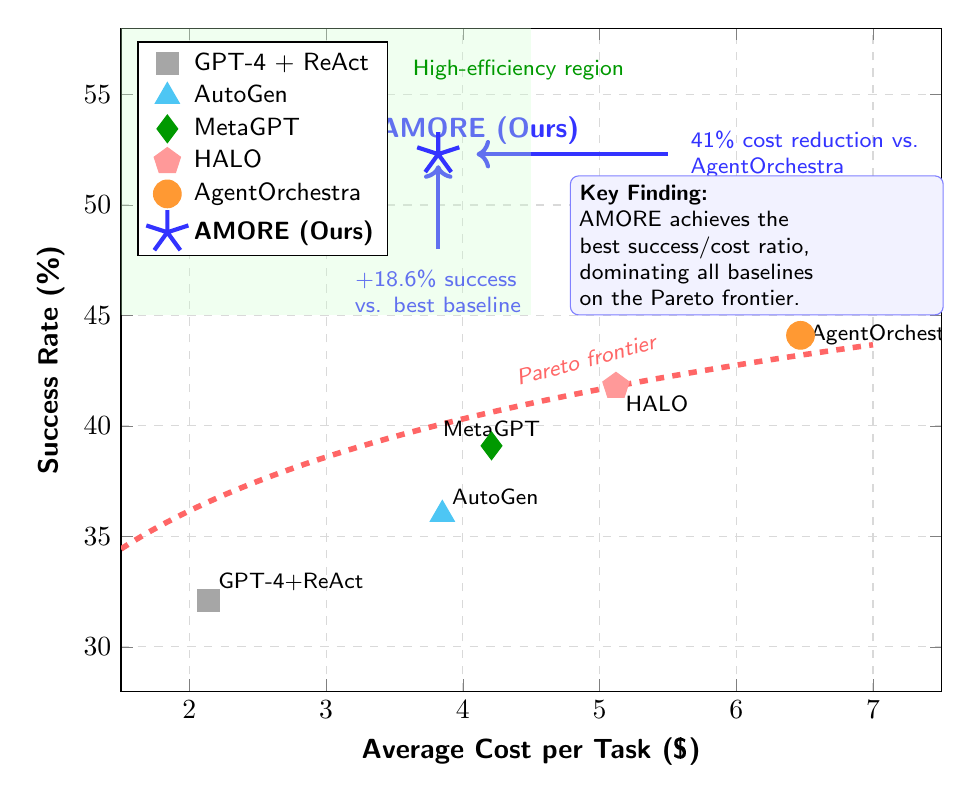
\begin{tikzpicture}
	\begin{axis}[
		width=12cm,
		height=10cm,
		xlabel={\textbf{Average Cost per Task (\$)}},
		ylabel={\textbf{Success Rate (\%)}},
		xmin=1.5,
		xmax=7.5,
		ymin=28,
		ymax=58,
		grid=both,
		grid style={dashed, gray!30},
		ylabel style={font=\sffamily\bfseries},
		xlabel style={font=\sffamily\bfseries},
		tick label style={font=\sffamily},
%		title={\sffamily\bfseries\large Cost-Performance Trade-off on MARS Benchmark},
		title style={yshift=8pt},
		legend style={
			at={(0.02,0.98)},
			anchor=north west,
			font=\sffamily\small,
			cells={anchor=west}
		}
		]
		% Scatter points for each method
		% GPT-4 + ReAct
		\addplot[
		only marks,
		mark=square*,
		mark size=4pt,
		color=gray!70
		] coordinates {(2.14, 32.1)};
		% AutoGen
		\addplot[
		only marks,
		mark=triangle*,
		mark size=5pt,
		color=cyan!70
		] coordinates {(3.85, 36.0)};
		% MetaGPT
		\addplot[
		only marks,
		mark=diamond*,
		mark size=5pt,
		color=green!60!black
		] coordinates {(4.21, 39.1)};
		% HALO
		\addplot[
		only marks,
		mark=pentagon*,
		mark size=5pt,
		color=pink!80!red
		] coordinates {(5.12, 41.8)};
		% AgentOrchestra
		\addplot[
		only marks,
		mark=otimes*,
		mark size=5pt,
		color=orange!80
		] coordinates {(6.47, 44.1)};
		% AMORE (Ours) - Highlighted with star
		\addplot[
		only marks,
		mark=star,
		mark size=8pt,
		color=blue!80,
		line width=1.5pt
		] coordinates {(3.82, 52.3)};
		% Pareto frontier (dashed line)
		\addplot[
		color=red!60,
		line width=2pt,
		dashed,
		domain=1.5:7,
		samples=100
		] {32 + 6*ln(x)};
		% Labels for each point
		\node[font=\sffamily\footnotesize, anchor=south west] at (axis cs:2.14,32.1) {GPT-4+ReAct};
		\node[font=\sffamily\footnotesize, anchor=south west] at (axis cs:3.85,36.0) {AutoGen};
		\node[font=\sffamily\footnotesize, anchor=south] at (axis cs:4.21,39.1) {MetaGPT};
		\node[font=\sffamily\footnotesize, anchor=north west] at (axis cs:5.12,41.8) {HALO};
		\node[font=\sffamily\footnotesize, anchor=west] at (axis cs:6.47,44.1) {AgentOrchestra};
		\node[font=\sffamily\bfseries, color=blue!80, anchor=south] at (axis cs:4.12,52.3) {\textbf{AMORE (Ours)}};
		% Annotation for AMORE's advantage
		\draw[->, line width=1.5pt, color=blue!80] (axis cs:5.5,52.3) -- (axis cs:4.1,52.3);
		\node[font=\sffamily\footnotesize, color=blue!80, anchor=west, text width=3cm] at (axis cs:5.6,52.3) {41\% cost reduction vs. AgentOrchestra};
		\draw[->, line width=1.5pt, color=blue!80] (axis cs:3.82,48) -- (axis cs:3.82,51.8);
		\node[font=\sffamily\footnotesize, color=blue!80, anchor=north, text width=2.5cm, align=center] at (axis cs:3.82,47.5) {+18.6\% success vs. best baseline};
		% Pareto frontier annotation
		\node[font=\sffamily\footnotesize\itshape, color=red!60, rotate=15] at (axis cs:4.9,43.0) {Pareto frontier};
		% Efficiency region annotation
		\fill[green!20, opacity=0.3] (axis cs:1.5,45) rectangle (axis cs:4.5,58);
		\node[font=\sffamily\footnotesize, color=green!60!black, anchor=north east] at (axis cs:5.25,57) {High-efficiency region};
		\legend{
			GPT-4 + ReAct,
			AutoGen,
			MetaGPT,
			HALO,
			AgentOrchestra,
			\textbf{AMORE (Ours)}
		}
	\end{axis}
	% Key insight box
	\node[draw=blue!50, fill=blue!5, rounded corners=3pt, font=\sffamily\footnotesize, text width=4.5cm, align=left, anchor=north west] at (5.7,6.55) {
		\textbf{Key Finding:}\\
		AMORE achieves the\\
		best success/cost ratio,\\
		dominating all baselines\\
		on the Pareto frontier.
	};
\end{tikzpicture}}
	\caption{Cost-Performance Trade-off on MARS Benchmark. AMORE achieves highest success rate at lower cost than hierarchical alternatives.}
	\label{fig:framework6}
\end{figure}

\subsection{Architecture Comparison}
\begin{figure}[h]
	\centering
	\input{figures/communication_efficiency_figure}
	\caption{Architecture comparison across multi-agent approaches.}
	\label{fig:framework6_}
\end{figure}

\begin{figure}[h]
	\centering
	% ============================================
% PART B: Quantitative Comparison (Bottom)
% ============================================
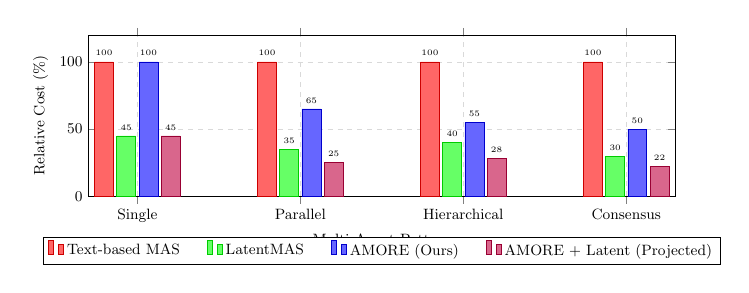
\begin{tikzpicture}[scale=0.6, transform shape]
	\begin{axis}[
		ybar,
		width=14cm,
		height=5cm,
		bar width=0.4cm,
		ylabel={Relative Cost (\%)},
		ylabel style={font=\small},
		xlabel={Multi-Agent Pattern},
		xlabel style={font=\small},
		symbolic x coords={Single, Parallel, Hierarchical, Consensus},
		xtick=data,
		xticklabel style={font=\small},
		yticklabel style={font=\small},
		ymin=0,
		ymax=120,
		legend style={
			at={(0.5,-0.25)},
			anchor=north,
			legend columns=4,
			font=\small,
			/tikz/every even column/.append style={column sep=0.5cm}
		},
		legend cell align={left},
		nodes near coords,
		nodes near coords style={font=\tiny, above},
		every node near coord/.append style={rotate=0},
		grid=major,
		grid style={dashed, gray!30},
		]
		
		\addplot[fill=red!60, draw=red!80!black] coordinates {
			(Single, 100) (Parallel, 100) (Hierarchical, 100) (Consensus, 100)
		};
		
		\addplot[fill=green!60, draw=green!80!black] coordinates {
			(Single, 45) (Parallel, 35) (Hierarchical, 40) (Consensus, 30)
		};
		
		\addplot[fill=blue!60, draw=blue!80!black] coordinates {
			(Single, 100) (Parallel, 65) (Hierarchical, 55) (Consensus, 50)
		};
		
		\addplot[fill=purple!60, draw=purple!80!black] coordinates {
			(Single, 45) (Parallel, 25) (Hierarchical, 28) (Consensus, 22)
		};
		
		\legend{Text-based MAS, LatentMAS, AMORE (Ours), AMORE + Latent (Projected)}
		
	\end{axis}
\end{tikzpicture}
	\caption{Quantitative comparison across multi-agent approaches.}
	\label{fig:framework6_1}
\end{figure}

\subsection{Ablation Study Visualization}
\begin{figure}[h]
	\centering
	\scalebox{0.55}{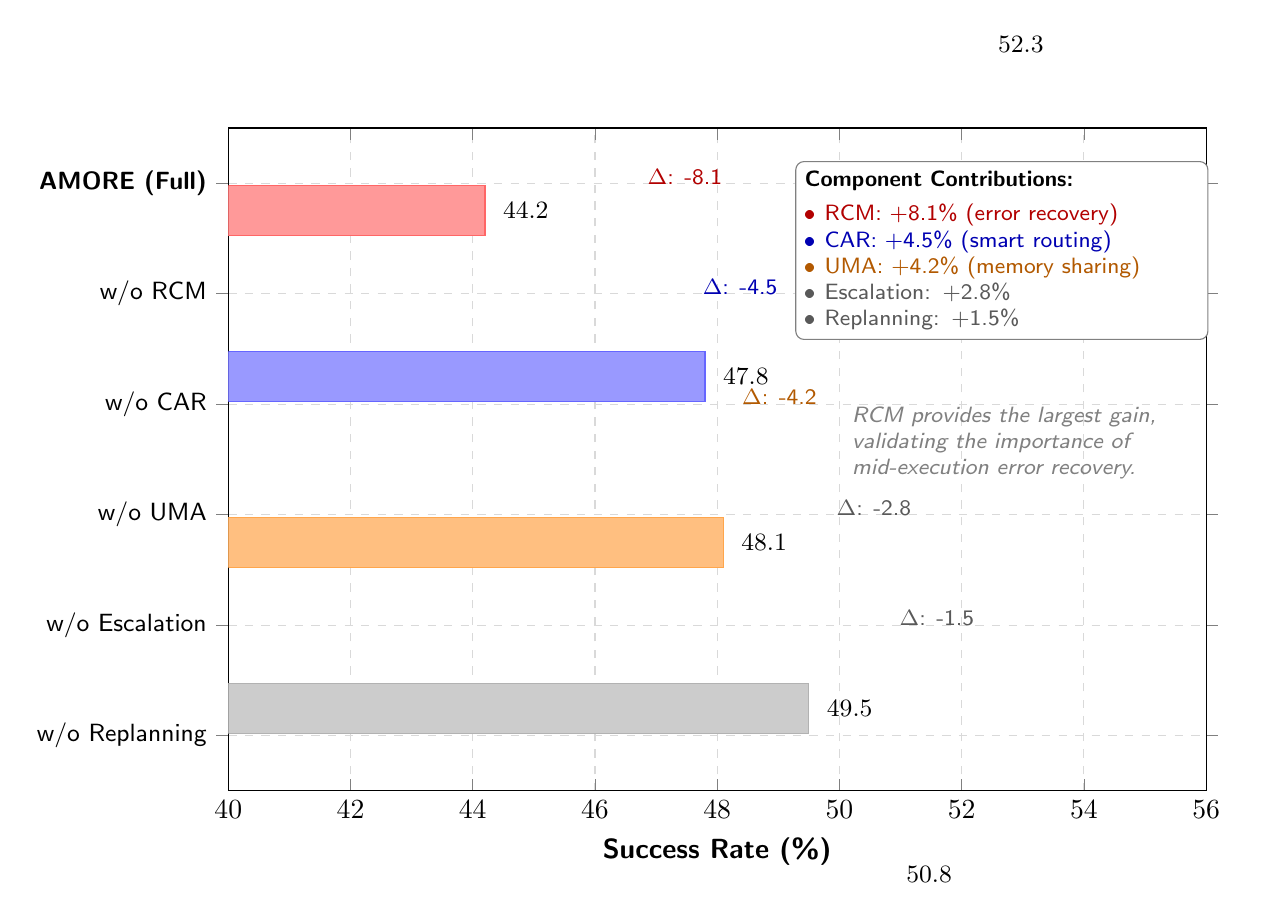
\begin{tikzpicture}
	\begin{axis}[
		xbar,
		bar width=18pt,
		width=14cm,
		height=10cm,
		xlabel={\textbf{Success Rate (\%)}},
		ylabel={},
		xmin=40,
		xmax=56,
		ytick={1,2,3,4,5,6},
		yticklabels={
			{w/o Replanning},
			{w/o Escalation},
			{w/o UMA},
			{w/o CAR},
			{w/o RCM},
			{\textbf{AMORE (Full)}}
		},
		y tick label style={font=\sffamily\small, anchor=east},
		xlabel style={font=\sffamily\bfseries},
		tick label style={font=\sffamily},
		grid=major,
		grid style={dashed, gray!30},
		title style={yshift=8pt},
		nodes near coords,
		nodes near coords style={font=\sffamily\small\bfseries, anchor=west, xshift=3pt},
		nodes near coords align={horizontal}
		]
		% Ablation results (ordered from bottom to top in the plot)
		\addplot[fill=gray!40, draw=gray!60] coordinates {(50.8, 1)};   % w/o Replanning
		\addplot[fill=gray!40, draw=gray!60] coordinates {(49.5, 2)};   % w/o Escalation
		\addplot[fill=orange!50, draw=orange!70] coordinates {(48.1, 3)};  % w/o UMA
		\addplot[fill=blue!40, draw=blue!60] coordinates {(47.8, 4)};    % w/o CAR
		\addplot[fill=red!40, draw=red!60] coordinates {(44.2, 5)};      % w/o RCM
		\addplot[fill=green!50, draw=green!70, postaction={pattern=north east lines, pattern color=white}] coordinates {(52.3, 6)};  % Full AMORE
	\end{axis}
	% Delta annotations
	\node[font=\sffamily\footnotesize, color=red!70!black] at (5.8,7.8) {$\Delta$: -8.1};
	\node[font=\sffamily\footnotesize, color=blue!70!black] at (6.5,6.4) {$\Delta$: -4.5};
	\node[font=\sffamily\footnotesize, color=orange!70!black] at (7.0,5.0) {$\Delta$: -4.2};
	\node[font=\sffamily\footnotesize, color=gray!70!black] at (8.2,3.6) {$\Delta$: -2.8};
	\node[font=\sffamily\footnotesize, color=gray!70!black] at (9.0,2.2) {$\Delta$: -1.5};
	% Component contribution box
	\node[draw=black!50, fill=white, rounded corners=3pt, font=\sffamily\footnotesize, text width=5cm, align=left, anchor=north west] at (7.2,8) {
		\textbf{Component Contributions:}\\[3pt]
		\textcolor{red!70!black}{\textbullet\ RCM: +8.1\% (error recovery)}\\
		\textcolor{blue!70!black}{\textbullet\ CAR: +4.5\% (smart routing)}\\
		\textcolor{orange!70!black}{\textbullet\ UMA: +4.2\% (memory sharing)}\\
		\textcolor{gray!70!black}{\textbullet\ Escalation: +2.8\%}\\
		\textcolor{gray!70!black}{\textbullet\ Replanning: +1.5\%}
	};
	% Insight
	\node[font=\sffamily\footnotesize\itshape, color=gray, text width=5cm, align=left, anchor=north west] at (7.8,5.0) {
		\textit{RCM provides the largest gain,\\
			validating the importance of\\
			mid-execution error recovery.}
	};
\end{tikzpicture}}
	\caption{Ablation Study Visualization on MARS Benchmark}
	\label{fig:framework7}
\end{figure}

\section{Extended Related Work}
\label{sec:extended_related}

This section provides a comprehensive survey of related work across six major research areas relevant to AMORE: LLM-based agents, multi-agent systems, task decomposition, memory architectures, agent communication protocols, and benchmarks.
\begin{algorithm}[t]
	\caption{\amore{} Execution Loop}
	\label{alg:amore}
	\small
	\begin{algorithmic}[1]
		\REQUIRE Task $\mathcal{T}$, Budget $B$, Agent Pool $\mathcal{A}$, Memory $M$
		\ENSURE Final Result $\mathcal{R}$
		\STATE $P \leftarrow \car{}.\text{CreatePlan}(\mathcal{T}, B, \mathcal{A})$
		\FOR{$(t, \pi, \text{agents})$ in $P$}
		\STATE $\text{context} \leftarrow \uma{}.\text{RetrieveRelevant}(t, M_E, M_S)$
		\STATE $o_t \leftarrow \text{Execute}(t, \pi, \text{agents}, \text{context})$
		\STATE $\uma{}.\text{Store}(M_E, (t, \pi, o_t, \text{metadata}))$
		\STATE $\text{action}, \text{update} \leftarrow \rcm{}.\text{Checkpoint}(o_t, t, \pi)$
		\IF{action = \textsc{Retry}}
		\STATE $o_t \leftarrow \text{Execute}(t, \pi, \text{agents}, \text{context})$
		\ELSIF{action = \textsc{Escalate}}
		\STATE $(t, \pi_{\text{new}}) \leftarrow \text{update}$
		\STATE $o_t \leftarrow \text{Execute}(t, \pi_{\text{new}}, \text{SelectAgents}(\pi_{\text{new}}))$
		\ELSIF{action = \textsc{Replan}}
		\STATE $P \leftarrow \text{update}$ \COMMENT{Replace remaining plan}
		\ENDIF
		\STATE $\text{results}[t] \leftarrow o_t$
		\ENDFOR
		\STATE $\uma{}.\text{Consolidate}(M_E \rightarrow M_S)$
		%		\RETURN $\text{Synthesize}(\text{results})$
		\STATE \textbf{return} $\text{Synthesize}(\text{results})$
	\end{algorithmic}
\end{algorithm}

% ==============================================================================
% 1. LLM-BASED AGENTS
% ==============================================================================
\subsection{LLM-Based Autonomous Agents}
\label{sec:related_llm_agents}

The emergence of Large Language Models as autonomous agents represents a paradigm shift in artificial intelligence \citep{xi2023rise, wang2024survey}. We organize this literature into four key capability areas.

\subsubsection{Reasoning and Planning}

\textbf{Chain-of-Thought Reasoning.} Wei et al. \citep{wei2022cot} demonstrated that prompting LLMs to generate intermediate reasoning steps dramatically improves performance on complex tasks. This foundational work spawned numerous extensions: Self-Consistency \citep{wang2023selfconsistency} improves reliability through majority voting over multiple reasoning paths; Zero-Shot CoT \citep{kojima2022large} shows that simply adding "Let's think step by step" elicits reasoning; and Least-to-Most prompting \citep{zhou2022least} decomposes complex problems into simpler subproblems.

\textbf{Tree and Graph Search.} Tree-of-Thoughts (ToT) \citep{yao2024tot} enables deliberate problem-solving by treating reasoning as search over a tree of potential thought sequences. Graph-of-Thoughts (GoT) \citep{besta2024graph} extends this to arbitrary graph structures, enabling more complex reasoning patterns. RAP (Reasoning via Planning) \citep{hao2023rap} combines LLMs with Monte Carlo Tree Search for improved planning.

\textbf{Test-Time Compute Scaling.} Recent work demonstrates that scaling compute at inference time can dramatically improve reasoning. OpenAI's o1 \citep{openai2024o1} achieves remarkable mathematical reasoning through learned chain-of-thought at scale. The survey by \citet{snell2024scaling} provides a comprehensive analysis of test-time compute scaling strategies.

\textbf{Reflection and Self-Correction.} Reflexion \citep{shinn2024reflexion} enables agents to learn from verbal feedback and past mistakes without weight updates. Self-Refine \citep{madaan2024selfrefine} iteratively improves outputs through self-feedback loops. CRITIC \citep{gou2024critic} uses tool-augmented self-verification for improved reasoning.

\subsubsection{Tool Use and Function Calling}

\textbf{Learning to Use Tools.} Toolformer \citep{schick2023toolformer} demonstrates that LLMs can learn to use tools through self-supervised learning on API calls. Gorilla \citep{patil2023gorilla} specializes in accurate API documentation understanding and reduces hallucination in function calls. ToolBench \citep{qin2024toolbench} provides a comprehensive benchmark spanning 16,000+ real-world APIs.

\textbf{Tool Selection and Composition.} AnyTool \citep{du2024anytool} addresses the challenge of selecting appropriate tools from large tool libraries. TaskMatrix.AI \citep{liang2023taskmatrix} connects LLMs with millions of APIs for diverse task completion. ToolkenGPT \citep{hao2024toolken} learns tool use through virtual tokens representing tools.

\textbf{Code Generation as Tool Use.} Program-aided Language Models (PAL) \citep{gao2023pal} use code generation as a reasoning tool. Code Interpreter paradigms (as in GPT-4) demonstrate the power of executable code for complex computations and data analysis.

\subsubsection{Memory and Context Management}

\textbf{Long-Context Handling.} While modern LLMs support longer contexts (128K+ tokens), effective utilization remains challenging. Lost in the Middle \citep{liu2024lost} shows LLMs struggle to use information in long contexts. Landmark Attention \citep{mohtashami2023landmark} and Focused Transformer \citep{tworkowski2023focused} propose architectural solutions for better long-range attention.

\textbf{External Memory Systems.} MemGPT \citep{packer2023memgpt} implements virtual context management through hierarchical memory, enabling infinite context through intelligent paging. Larimar \citep{das2024larimar} (ICML 2024) introduces episodic memory control for LLMs, enabling selective memory retrieval and storage.

\textbf{Memory Taxonomies.} The comprehensive survey by \citet{zhang2025memory} categorizes agent memory into working memory (current task context), episodic memory (past experiences), and semantic memory (consolidated knowledge). Our UMA architecture draws directly from this taxonomy.

\subsubsection{Grounding and Environment Interaction}

\textbf{The ReAct Framework.} ReAct \citep{yao2023react} interleaves reasoning traces with actions, enabling LLMs to interact with external environments while maintaining interpretable reasoning. This foundational framework underlies most modern agent systems.

\textbf{Embodied Agents.} SayCan \citep{ahn2022saycan} grounds LLM knowledge in robot affordances for real-world task execution. PaLM-E \citep{driess2023palme} directly incorporates visual and embodied inputs into language model reasoning. RT-2 \citep{brohan2023rt2} demonstrates vision-language-action models for robotic control.

\textbf{Web Agents.} WebGPT \citep{nakano2022webgpt} enables LLMs to search and cite sources for improved factual accuracy. Mind2Web \citep{deng2023mind2web} provides a large-scale dataset for generalist web agents. WebArena \citep{zhou2024webarena} benchmarks autonomous web task completion.

% ==============================================================================
% 2. MULTI-AGENT SYSTEMS
% ==============================================================================
\subsection{Multi-Agent LLM Systems}
\label{sec:related_llm}

Multi-agent collaboration extends single-agent capabilities through diverse coordination patterns.

\subsubsection{Conversational Multi-Agent Frameworks}

\textbf{AutoGen.} Microsoft's AutoGen \citep{wu2023autogen} enables conversational multi-agent programming with flexible agent definitions, customizable conversation patterns, and human-in-the-loop integration. AutoGen has become a foundational framework for multi-agent research and applications.

\textbf{CAMEL.} Li et al. \citep{li2023camel} introduced role-playing for cooperative agents, demonstrating that assigning distinct roles improves task completion through emergent social behaviors. Follow-up work explores inception prompting and society of agents.

\textbf{ChatDev.} Qian et al. \citep{qian2023chatdev} simulates a virtual software company with CEO, CTO, programmer, and tester agents collaborating through chat-based communication. This approach demonstrates the power of role-based decomposition for software engineering.

\subsubsection{Hierarchical and Orchestrated Systems}

\textbf{HALO.} Chen et al. \citep{chen2025halo} propose three-tier orchestration with high-level strategic planners, mid-level tactical coordinators, and low-level task executors. This hierarchical structure handles complex tasks through principled delegation.

\textbf{AgentOrchestra.} Liu et al. \citep{liu2025agentorchestra} implements a conductor-specialist model where a central conductor orchestrates domain specialists using the TEA (Tool-Environment-Agent) protocol. This approach achieves strong results on complex benchmarks.

\textbf{MetaGPT.} Hong et al. \citep{hong2024metagpt} (ICLR 2024) encodes Standard Operating Procedures (SOPs) to structure multi-agent collaboration for software development. Role-specific prompts and message passing enable realistic team dynamics.

\textbf{MDAgents.} Kim et al. \citep{kim2024mdagents} (NeurIPS 2024) demonstrates adaptive collaboration for medical tasks, showing that different medical queries require different agent configurations. This work directly motivates our adaptive orchestration approach.

\subsubsection{Debate and Deliberation}

\textbf{Multi-Agent Debate.} Du et al. \citep{du2023multiagent} show that having multiple LLM agents debate improves factuality and reasoning. The debate structure encourages agents to critique and refine each other's responses.

\textbf{Society of Mind.} Zhuge et al. \citep{zhuge2023mindstorms} propose Mindstorms, where agents with different personas collaborate through structured discussion. This work explores how diversity in agent perspectives improves problem-solving.

\textbf{Exchange-of-Thought.} Yin et al. \citep{yin2023exchange} introduces a framework for agents to exchange intermediate reasoning, enabling collaborative problem-solving that outperforms individual reasoning.

\subsubsection{Emergent Behaviors}

\textbf{Generative Agents.} Park et al. \citep{park2023generative} demonstrate emergent social behaviors in a simulated town populated by LLM agents. Agents form relationships, spread information, and coordinate activities without explicit programming.

\textbf{Agent Cooperation and Competition.} Zhang et al. \citep{zhang2023exploring} explore how multi-agent systems exhibit cooperative and competitive behaviors, finding that appropriate incentive structures dramatically affect outcomes.

\subsubsection{Key Gap Addressed by AMORE}

Existing multi-agent systems use \textbf{static} orchestration patterns---the coordination structure is fixed at design time. AMORE addresses this by dynamically selecting orchestration patterns based on task complexity, enabling efficient resource allocation while maintaining high success rates.

%\paragraph{Latent-Space Collaboration.}
%Recent work by ~\citet{zou2025latent} proposes LatentMAS, which moves
%agent collaboration from token space into the model's latent space. Rather than
%exchanging textual reasoning traces, agents communicate through latent representations,
%achieving 50--80\% token reduction and 3--7$\times$ wall-clock speedup without training.
%While LatentMAS optimizes \emph{how} agents communicate, AMORE addresses \emph{when}
%and \emph{which pattern} of collaboration is optimal---these approaches are complementary
%and could be integrated for both efficient communication and adaptive orchestration (Figure \ref{fig:framework6_}).

% ==============================================================================
% 3. TASK DECOMPOSITION AND PLANNING
% ==============================================================================
\subsection{Task Decomposition and Planning}
\label{sec:related_decomposition}

Effective task decomposition is critical for both single and multi-agent success.

\subsubsection{Static Decomposition}

\textbf{HuggingGPT.} Shen et al. \citep{shen2023hugginggpt} use GPT-4 to decompose tasks and route subtasks to specialized Hugging Face models. This demonstrates the power of LLM-based planning combined with specialized execution.

\textbf{ViperGPT.} Surís et al. \citep{suris2023vipergpt} generates Python programs that compose vision-language models for complex visual reasoning. The generated programs serve as executable task decompositions.

\subsubsection{Adaptive Decomposition}

\textbf{ADaPT.} Prasad et al. \citep{prasad2024adapt} (NAACL 2024) introduces decomposition as-needed based on LLM capability assessment. Tasks are decomposed only when the current agent cannot handle them, achieving 28.3\% improvement on ALFWorld.

\textbf{TDAG.} Zhang et al. \citep{zhang2025tdag} dynamically generates task-specific subagents with an evolving skill library. New skills are learned and stored for future reuse, enabling continual improvement.

\textbf{Self-Discover.} Zhou et al. \citep{zhou2024selfdiscover} enables LLMs to discover task-specific reasoning structures, combining atomic reasoning modules into coherent strategies without manual prompting.

\subsubsection{Planning Under Uncertainty}

\textbf{RAP (Reasoning via Planning).} Hao et al. \citep{hao2023rap} combines LLMs with MCTS for strategic planning under uncertainty. The world model enables lookahead search for improved decision-making.

\textbf{LLM+P.} Liu et al. \citep{liu2023llmp} combines LLM commonsense with classical planners for robust planning. The hybrid approach leverages complementary strengths of neural and symbolic systems.

\textbf{ISR-LLM.} Zhou et al. \citep{zhou2024isr} introduces iterative self-refinement for LLM planning, using execution feedback to improve plan quality.

\subsubsection{Complexity Estimation}

\textbf{Complexity-Aware Methods.} While not directly predicting orchestration patterns, prior work on difficulty estimation informs our CAR design. \citet{sakaguchi2021winogrande} demonstrate adversarial filtering based on difficulty. \citet{swayamdipta2020dataset} introduce dataset cartography for understanding example difficulty.

\textbf{Capability Assessment.} ADaPT \citep{prasad2024adapt} includes implicit capability assessment---decomposing when the model "cannot handle" a task. We make this explicit through learned complexity prediction.

% ==============================================================================
% 4. MEMORY AND RETRIEVAL
% ==============================================================================
\subsection{Memory Architectures and Retrieval}
\label{sec:related_memory}

Memory systems enable agents to leverage past experiences and external knowledge.

\subsubsection{Retrieval-Augmented Generation}

\textbf{RAG Foundations.} Lewis et al. \citep{lewis2020rag} introduced Retrieval-Augmented Generation, combining parametric and non-parametric memory. RAG enables LLMs to access external knowledge bases for improved factuality.

\textbf{Advanced RAG.} Recent work improves RAG through query rewriting \citep{ma2023query}, multi-step retrieval \citep{trivedi2023interleaving}, and self-reflective retrieval \citep{asai2023selfrag}. The comprehensive survey by \citet{gao2023rag} covers the RAG landscape.

\textbf{Agentic RAG.} Combining agents with RAG enables more sophisticated information seeking. CRAG \citep{yan2024corrective} uses web search to correct retrieval errors. Adaptive-RAG \citep{jeong2024adaptive} dynamically adjusts retrieval strategy based on query complexity.

\subsubsection{Episodic Memory for Agents}

\textbf{Larimar.} Das et al. \citep{das2024larimar} (ICML 2024) introduces episodic memory control for LLMs, enabling selective storage and retrieval of past experiences. This work directly influences our UMA episodic tier design.

\textbf{Generative Agent Memory.} Park et al. \citep{park2023generative} implement memory stream, reflection, and planning components for believable agent behavior. The reflection mechanism consolidates experiences into higher-level insights.

\textbf{RecurrentGPT.} Zhou et al. \citep{zhou2023recurrentgpt} maintains a dynamic memory structure for long-form text generation, demonstrating the importance of structured memory for coherent long-horizon tasks.

\subsubsection{Knowledge Graphs and Structured Memory}

\textbf{Think-on-Graph.} Sun et al. \citep{sun2024thinkongraph} enables LLMs to reason over knowledge graphs through iterative graph exploration. This combines structured knowledge with flexible reasoning.

\textbf{GraphRAG.} Microsoft's GraphRAG \citep{edge2024graphrag} builds hierarchical knowledge graphs from documents, enabling multi-scale summarization and question answering beyond traditional RAG.

\subsubsection{Memory Consolidation}

\textbf{Sleep-Like Consolidation.} Inspired by biological memory consolidation, \citet{schrittwieser2020mastering} show how experience replay improves learning. We adapt this principle for episodic-to-semantic memory transfer.

% ==============================================================================
% 5. AGENT COMMUNICATION PROTOCOLS
% ==============================================================================
\subsection{Agent Communication Protocols}
\label{sec:related_protocols}

Standardized communication enables agent interoperability and scalability.

\subsubsection{Industry Standards}

\textbf{A2A Protocol.} Google's Agent-to-Agent (A2A) Protocol \citep{google2025a2a} enables peer-to-peer agent communication with agent cards describing capabilities, supported tasks, and interaction patterns. A2A is designed for open ecosystems where agents from different providers collaborate.

\textbf{Model Context Protocol (MCP).} Anthropic's MCP \citep{anthropic2024mcp} standardizes tool invocation and context sharing across frameworks. MCP provides a unified interface for agents to access tools and data sources.

\textbf{Agent Communication Protocol (ACP).} IBM's ACP \citep{ibm2025acp} provides workflow orchestration primitives including task assignment, progress tracking, and error handling for enterprise multi-agent deployments.

\textbf{Agent Network Protocol (ANP).} The Agent Network Protocol \citep{anp2025} focuses on decentralized agent networks with reputation systems and trust management.

\subsubsection{Research Protocols}

\textbf{AgentProtocol.} Open-source efforts like AgentProtocol aim to standardize agent API interfaces for benchmarking and evaluation consistency.

\textbf{LMQL.} Beurer-Kellner et al. \citep{beurer2023lmql} introduce a query language for LLMs, enabling structured interaction patterns that could generalize to multi-agent communication.

\subsubsection{Implications for AMORE}

AMORE is designed to be protocol-agnostic, with adapter layers for A2A, MCP, and ACP integration. Our cross-agent memory sharing can leverage these protocols for standardized communication.

% ==============================================================================
% 6. BENCHMARKS AND EVALUATION
% ==============================================================================
\subsection{Agent Benchmarks and Evaluation}
\label{sec:related_benchmarks}

Rigorous evaluation requires comprehensive benchmarks across diverse capabilities.

\subsubsection{General Agent Benchmarks}

\textbf{AgentBench.} Liu et al. \citep{liu2024agentbench} (ICLR 2024) evaluates LLM-as-Agent across 8 environments: Operating System, Database, Knowledge Graph, Card Game, Lateral Thinking, House-Holding, Web Shopping, and Web Browsing. Comprehensive evaluation of 29 models reveals significant capability gaps.

\textbf{MINT.} Wang et al. \citep{wang2024mint} provides a multi-turn interactive benchmark covering diverse reasoning, tool use, and information seeking capabilities.

\textbf{GAIA.} Mialon et al. \citep{mialon2023gaia} benchmarks general AI assistants on tasks requiring real-world knowledge, multi-step reasoning, and web interaction.

\subsubsection{Web and Computer Use}

\textbf{WebArena.} Zhou et al. \citep{zhou2024webarena} provides realistic, reproducible web environments for agent evaluation across shopping, forums, GitLab, and content management systems.

\textbf{OSWorld.} Xie et al. \citep{xie2024osworld} benchmarks multimodal agents in real computer environments (Ubuntu, Windows, macOS), requiring screenshot understanding and diverse software interaction.

\textbf{Mind2Web.} Deng et al. \citep{deng2023mind2web} provides a large-scale dataset for generalist web agents with tasks spanning 137 websites across 31 domains.

\subsubsection{Software Engineering}

\textbf{SWE-bench.} Jimenez et al. \citep{jimenez2024swebench} evaluates agents on real GitHub issues from popular Python repositories, requiring code understanding, localization, and patch generation.

\textbf{HumanEval/MBPP.} While not agent-specific, these code generation benchmarks \citep{chen2021evaluating, austin2021program} remain important baselines for coding capability assessment.

\textbf{DevBench.} Li et al. \citep{li2024devbench} evaluates LLMs across the full software development lifecycle including requirements, design, implementation, and testing.

\subsubsection{Domain-Specific Benchmarks}

\textbf{MedAgentBench.} Evaluates medical question answering and clinical decision support capabilities for healthcare applications.

\textbf{FinanceBench.} Islam et al. \citep{islam2024financebench} tests financial analysis and reasoning on real-world financial documents.

\textbf{ScienceQA.} Lu et al. \citep{lu2022scienceqa} provides multimodal science questions requiring reasoning across physics, chemistry, and biology.

\subsubsection{Multi-Agent Evaluation Gap}

\begin{figure*}[t]
	\centering
	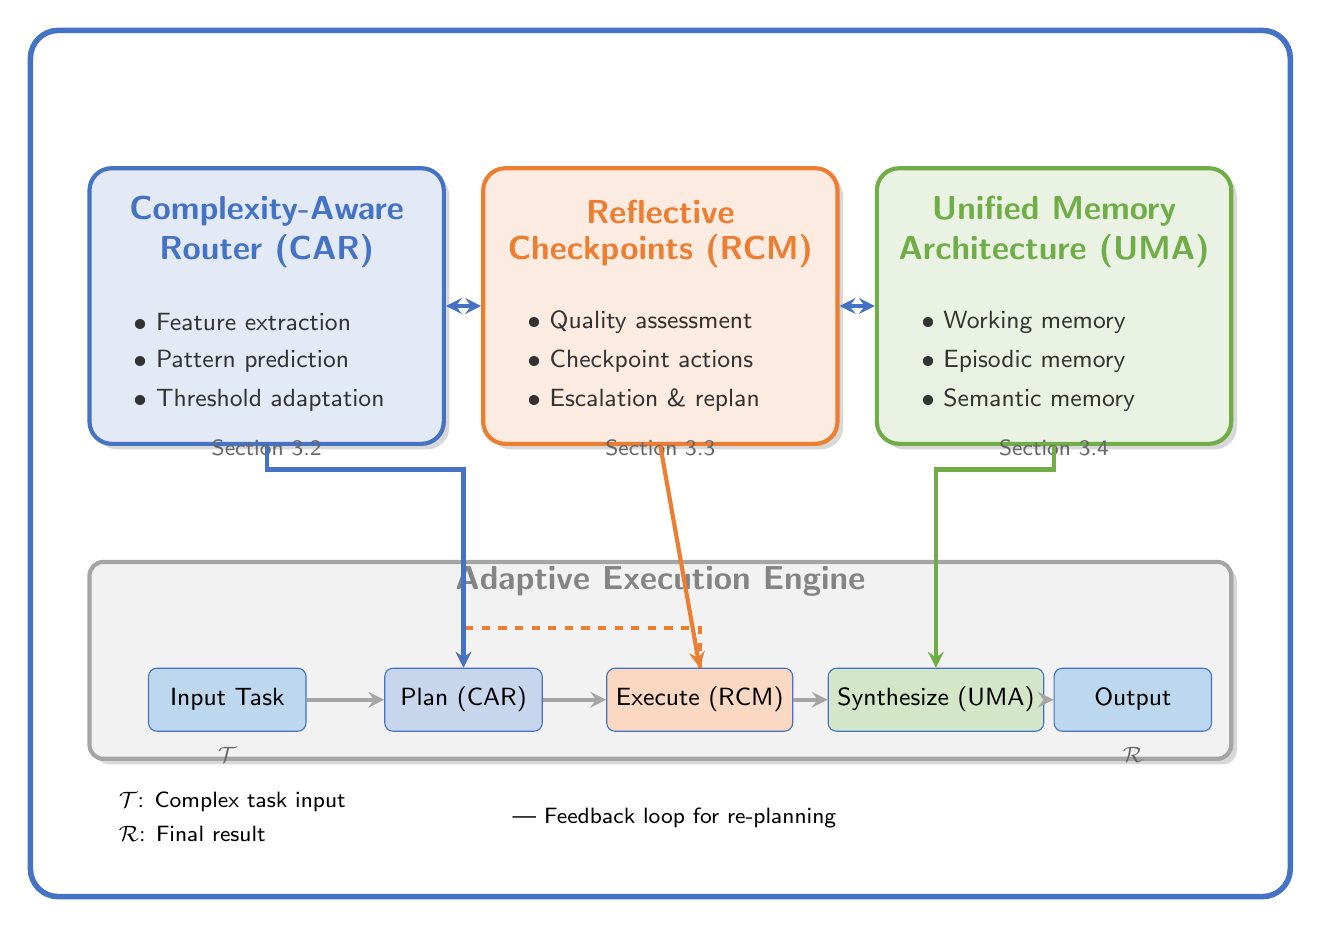
\begin{tikzpicture}[
	% Node styles
	component/.style={
		rectangle,
		rounded corners=8pt,
		draw=#1,
		fill=#1!15,
		line width=1.5pt,
		minimum width=4.5cm,
		minimum height=3.5cm,
		text centered,
		font=\sffamily\bfseries,
		drop shadow={shadow xshift=2pt, shadow yshift=-2pt, opacity=0.3}
	},
	subitem/.style={
		font=\sffamily\small,
		text=black!80
	},
	engine/.style={
		rectangle,
		rounded corners=5pt,
		draw=amoregray,
		fill=amorelightgray,
		line width=1.5pt,
		minimum width=14.5cm,
		minimum height=2.5cm,
		text centered,
		font=\sffamily\bfseries,
		drop shadow={shadow xshift=2pt, shadow yshift=-2pt, opacity=0.3}
	},
	mainbox/.style={
		rectangle,
		rounded corners=10pt,
		draw=amoreblue,
		fill=white,
		line width=2pt,
		inner sep=15pt
	},
	arrow/.style={
		->,
		>=stealth,
		line width=1.5pt,
		color=amoregray
	},
	doublearrow/.style={
		<->,
		>=stealth,
		line width=1.5pt,
		color=amoreblue
	},
	flowbox/.style={
		rectangle,
		rounded corners=3pt,
		draw=amoreblue,
		fill=amorelightblue,
		minimum width=2cm,
		minimum height=0.8cm,
		font=\sffamily\small
	},
	label/.style={
		font=\sffamily\footnotesize,
		color=black!60
	}
	]
	
	% Main container
	\node[mainbox, minimum width=16cm, minimum height=11cm] (mainframe) at (0,0) {};
	
	% Title
%	\node[font=\sffamily\Large\bfseries, color=amoreblue] at (0,5) {AMORE Framework};
	
	% Three main components
	\node[component=amoreblue] (car) at (-5,2) {};
	\node[font=\sffamily\bfseries\large, color=amoreblue] at (-5,3.2) {Complexity-Aware};
	\node[font=\sffamily\bfseries\large, color=amoreblue] at (-5,2.7) {Router (CAR)};
	\node[subitem, anchor=west] at (-6.8,1.8) {\textbullet\ Feature extraction};
	\node[subitem, anchor=west] at (-6.8,1.3) {\textbullet\ Pattern prediction};
	\node[subitem, anchor=west] at (-6.8,0.8) {\textbullet\ Threshold adaptation};
	\node[label] at (-5,0.2) {Section 3.2};
	
	\node[component=amoreorange] (rcm) at (0,2) {};
	\node[font=\sffamily\bfseries\large, color=amoreorange] at (0,3.2) {Reflective};
	\node[font=\sffamily\bfseries\large, color=amoreorange] at (0,2.7) {Checkpoints (RCM)};
	\node[subitem, anchor=west] at (-1.8,1.8) {\textbullet\ Quality assessment};
	\node[subitem, anchor=west] at (-1.8,1.3) {\textbullet\ Checkpoint actions};
	\node[subitem, anchor=west] at (-1.8,0.8) {\textbullet\ Escalation \& replan};
	\node[label] at (0,0.2) {Section 3.3};
	
	\node[component=amoregreen] (uma) at (5,2) {};
	\node[font=\sffamily\bfseries\large, color=amoregreen] at (5,3.2) {Unified Memory};
	\node[font=\sffamily\bfseries\large, color=amoregreen] at (5,2.7) {Architecture (UMA)};
	\node[subitem, anchor=west] at (3.2,1.8) {\textbullet\ Working memory};
	\node[subitem, anchor=west] at (3.2,1.3) {\textbullet\ Episodic memory};
	\node[subitem, anchor=west] at (3.2,0.8) {\textbullet\ Semantic memory};
	\node[label] at (5,0.2) {Section 3.4};
	
	% Connecting arrows between components
	\draw[doublearrow] (car.east) -- (rcm.west);
	\draw[doublearrow] (rcm.east) -- (uma.west);
	
	% Adaptive Execution Engine
	\node[engine] (engine) at (0,-2.5) {};
	\node[font=\sffamily\bfseries\large, color=amoregray!80!black] at (0,-1.5) {Adaptive Execution Engine};
	
	% Flow inside engine
	\node[flowbox] (input) at (-5.5,-3) {Input Task};
	\node[flowbox, fill=amoreblue!30] (plan) at (-2.5,-3) {Plan (CAR)};
	\node[flowbox, fill=amoreorange!30] (execute) at (0.5,-3) {Execute (RCM)};
	\node[flowbox, fill=amoregreen!30] (synthesize) at (3.5,-3) {Synthesize (UMA)};
	\node[flowbox] (output) at (6,-3) {Output};
	
	\draw[arrow] (input) -- (plan);
	\draw[arrow] (plan) -- (execute);
	\draw[arrow] (execute) -- (synthesize);
	\draw[arrow] (synthesize) -- (output);
	
	% Feedback loop
	\draw[arrow, dashed, color=amoreorange] (execute.north) -- ++(0,0.5) -| (plan.north);
	
	% Vertical arrows from components to engine
	\draw[arrow, color=amoreblue] (car.south) -- ++(0,-0.3) -| (plan.north);
	\draw[arrow, color=amoreorange] (rcm.south) -- (execute.north);
	\draw[arrow, color=amoregreen] (uma.south) -- ++(0,-0.3) -| (synthesize.north);
	
	% Labels
	\node[label] at (-5.5,-3.7) {$\mathcal{T}$};
	\node[label] at (6,-3.7) {$\mathcal{R}$};
	
	% Legend
	\node[font=\sffamily\footnotesize, anchor=west] at (-7,-4.3) {$\mathcal{T}$: Complex task input};
	\node[font=\sffamily\footnotesize, anchor=west] at (-7,-4.7) {$\mathcal{R}$: Final result};
	\node[font=\sffamily\footnotesize, anchor=west] at (-2,-4.5) {--- Feedback loop for re-planning};
	
\end{tikzpicture}
	\caption{Overview of the extended \amore{} framework. A high-level architecture diagram showing three main components (CAR, RCM, UMA) connected to a central "Adaptive Execution Engine. \car{} predicts optimal orchestration patterns, \rcm{} enables mid-execution adaptation through quality gates, and \uma{} provides cross-agent memory coherence.}
	\label{fig:framework1}
\end{figure*}

%
%\begin{figure*}
%\begin{tikzpicture}[
%	% Node styles
%	component/.style={
%		rectangle,
%		rounded corners=8pt,
%		draw=#1,
%		fill=#1!15,
%		line width=1.5pt,
%		minimum width=4.5cm,
%		minimum height=3.5cm,
%		text centered,
%		font=\sffamily\bfseries,
%		drop shadow={shadow xshift=2pt, shadow yshift=-2pt, opacity=0.3}
%	},
%	subitem/.style={
%		font=\sffamily\small,
%		text=black!80
%	},
%	engine/.style={
%		rectangle,
%		rounded corners=5pt,
%		draw=amoregray,
%		fill=amorelightgray,
%		line width=1.5pt,
%		minimum width=14.5cm,
%		minimum height=2.5cm,
%		text centered,
%		font=\sffamily\bfseries,
%		drop shadow={shadow xshift=2pt, shadow yshift=-2pt, opacity=0.3}
%	},
%	mainbox/.style={
%		rectangle,
%		rounded corners=10pt,
%		draw=amoreblue,
%		fill=white,
%		line width=2pt,
%		inner sep=15pt
%	},
%	arrow/.style={
%		->,
%		>=stealth,
%		line width=1.5pt,
%		color=amoregray
%	},
%	doublearrow/.style={
%		<->,
%		>=stealth,
%		line width=1.5pt,
%		color=amoreblue
%	},
%	flowbox/.style={
%		rectangle,
%		rounded corners=3pt,
%		draw=amoreblue,
%		fill=amorelightblue,
%		minimum width=2cm,
%		minimum height=0.8cm,
%		font=\sffamily\small
%	},
%	label/.style={
%		font=\sffamily\footnotesize,
%		color=black!60
%	}
%	]
%	
%	% Main container
%	\node[mainbox, minimum width=16cm, minimum height=11cm] (mainframe) at (0,0) {};
%	
%	% Title
%	\node[font=\sffamily\Large\bfseries, color=amoreblue] at (0,5) {AMORE Framework};
%	
%	% Three main components
%	\node[component=amoreblue] (car) at (-5,2) {};
%	\node[font=\sffamily\bfseries\large, color=amoreblue] at (-5,3.2) {Complexity-Aware};
%	\node[font=\sffamily\bfseries\large, color=amoreblue] at (-5,2.7) {Router (CAR)};
%	\node[subitem, anchor=west] at (-6.8,1.8) {\textbullet\ Feature extraction};
%	\node[subitem, anchor=west] at (-6.8,1.3) {\textbullet\ Pattern prediction};
%	\node[subitem, anchor=west] at (-6.8,0.8) {\textbullet\ Threshold adaptation};
%	\node[label] at (-5,0.2) {Section 3.2};
%	
%	\node[component=amoreorange] (rcm) at (0,2) {};
%	\node[font=\sffamily\bfseries\large, color=amoreorange] at (0,3.2) {Reflective};
%	\node[font=\sffamily\bfseries\large, color=amoreorange] at (0,2.7) {Checkpoints (RCM)};
%	\node[subitem, anchor=west] at (-1.8,1.8) {\textbullet\ Quality assessment};
%	\node[subitem, anchor=west] at (-1.8,1.3) {\textbullet\ Checkpoint actions};
%	\node[subitem, anchor=west] at (-1.8,0.8) {\textbullet\ Escalation \& replan};
%	\node[label] at (0,0.2) {Section 3.3};
%	
%	\node[component=amoregreen] (uma) at (5,2) {};
%	\node[font=\sffamily\bfseries\large, color=amoregreen] at (5,3.2) {Unified Memory};
%	\node[font=\sffamily\bfseries\large, color=amoregreen] at (5,2.7) {Architecture (UMA)};
%	\node[subitem, anchor=west] at (3.2,1.8) {\textbullet\ Working memory};
%	\node[subitem, anchor=west] at (3.2,1.3) {\textbullet\ Episodic memory};
%	\node[subitem, anchor=west] at (3.2,0.8) {\textbullet\ Semantic memory};
%	\node[label] at (5,0.2) {Section 3.4};
%	
%	% Connecting arrows between components
%	\draw[doublearrow] (car.east) -- (rcm.west);
%	\draw[doublearrow] (rcm.east) -- (uma.west);
%	
%	% Adaptive Execution Engine
%	\node[engine] (engine) at (0,-2.5) {};
%	\node[font=\sffamily\bfseries\large, color=amoregray!80!black] at (0,-1.5) {Adaptive Execution Engine};
%	
%	% Flow inside engine
%	\node[flowbox] (input) at (-5.5,-3) {Input Task};
%	\node[flowbox, fill=amoreblue!30] (plan) at (-2.5,-3) {Plan (CAR)};
%	\node[flowbox, fill=amoreorange!30] (execute) at (0.5,-3) {Execute (RCM)};
%	\node[flowbox, fill=amoregreen!30] (synthesize) at (3.5,-3) {Synthesize (UMA)};
%	\node[flowbox] (output) at (6,-3) {Output};
%	
%	\draw[arrow] (input) -- (plan);
%	\draw[arrow] (plan) -- (execute);
%	\draw[arrow] (execute) -- (synthesize);
%	\draw[arrow] (synthesize) -- (output);
%	
%	% Feedback loop
%	\draw[arrow, dashed, color=amoreorange] (execute.north) -- ++(0,0.5) -| (plan.north);
%	
%	% Vertical arrows from components to engine
%	\draw[arrow, color=amoreblue] (car.south) -- ++(0,-0.3) -| (plan.north);
%	\draw[arrow, color=amoreorange] (rcm.south) -- (execute.north);
%	\draw[arrow, color=amoregreen] (uma.south) -- ++(0,-0.3) -| (synthesize.north);
%	
%	% Labels
%	\node[label] at (-5.5,-3.7) {$\mathcal{T}$};
%	\node[label] at (6,-3.7) {$\mathcal{R}$};
%	
%	% Legend
%	\node[font=\sffamily\footnotesize, anchor=west] at (-7,-4.3) {$\mathcal{T}$: Complex task input};
%	\node[font=\sffamily\footnotesize, anchor=west] at (-7,-4.7) {$\mathcal{R}$: Final result};
%	\node[font=\sffamily\footnotesize, anchor=west] at (-2,-4.5) {--- Feedback loop for re-planning};
%	
%\end{tikzpicture}
%	
%\caption{Overview of the \amore{} framework. A high-level architecture diagram showing three main components (CAR, RCM, UMA) connected to a central "Adaptive Execution Engine. \car{} predicts optimal orchestration patterns, \rcm{} enables mid-execution adaptation through quality gates, and \uma{} provides cross-agent memory coherence.}
%\label{fig:framework1}
%\end{figure*}

Existing benchmarks primarily evaluate single-agent capabilities. Even benchmarks like AgentBench focus on individual agent performance. Our MARS benchmark addresses this gap by explicitly evaluating:
\begin{itemize}
	\item \textbf{Orchestration accuracy:} Whether the system selects optimal coordination patterns
	\item \textbf{Adaptation rate:} Whether mid-execution adjustments improve outcomes
	\item \textbf{Memory utilization:} Whether retrieved information is effectively used
	\item \textbf{Collaboration efficiency:} Whether multi-agent collaboration provides proportional value
\end{itemize}

% ==============================================================================
% 7. POSITIONING OF AMORE
% ==============================================================================
\subsection{Positioning of AMORE}
\label{sec:positioning}

Table~\ref{tab:positioning} positions AMORE relative to key prior work across multiple dimensions.

\begin{table*}[t]
	\centering
	\caption{Positioning of AMORE relative to prior work. \checkmark = fully supported, $\circ$ = partially supported, - = not supported.}
	\label{tab:positioning}
	\small
	\begin{tabular}{@{}lccccccc@{}}
		\toprule
		\textbf{Method} & \textbf{Multi-Agent} & \textbf{Adaptive} & \textbf{Checkpoints} & \textbf{Unified Memory} & \textbf{Complexity} & \textbf{Cost} \\
		& & \textbf{Orchestration} & & & \textbf{Prediction} & \textbf{Aware} \\
		\midrule
		ReAct \citep{yao2023react} & - & - & - & - & - & - \\
		AutoGen \citep{wu2023autogen} & \checkmark & - & - & $\circ$ & - & - \\
		MetaGPT \citep{hong2024metagpt} & \checkmark & - & - & $\circ$ & - & - \\
		HALO \citep{chen2025halo} & \checkmark & $\circ$ & - & - & - & $\circ$ \\
		AgentOrchestra \citep{liu2025agentorchestra} & \checkmark & - & - & $\circ$ & - & - \\
		ADaPT \citep{prasad2024adapt} & - & $\circ$ & - & - & $\circ$ & - \\
		MDAgents \citep{kim2024mdagents} & \checkmark & $\circ$ & - & - & $\circ$ & - \\
		LatentMAS \citep{zou2025latent} & \checkmark & - & - & $\circ$ & $-$ & \checkmark \\
		\midrule
		\textbf{AMORE (Ours)} & \checkmark & \checkmark & \checkmark & \checkmark & \checkmark & \checkmark \\
		\bottomrule
	\end{tabular}
\end{table*}

\begin{figure*}[t]
	\centering
	\definecolor{gpt4color}{RGB}{169,169,169}
\definecolor{autogencolor}{RGB}{135,206,235}
\definecolor{metagptcolor}{RGB}{144,238,144}
\definecolor{halocolor}{RGB}{255,182,193}
\definecolor{orchestracolor}{RGB}{255,218,185}
\definecolor{amorecolor}{RGB}{68,114,196}

\begin{tikzpicture}
	\begin{axis}[
		ybar,
		bar width=8pt,
		width=16cm,
		height=10cm,
		xlabel={\textbf{Environment}},
		ylabel={\textbf{Success Rate (\%)}},
		symbolic x coords={OS, DB, KG, Games, LTP, House, WebShop, WebBrowse, Average},
		xtick=data,
		x tick label style={rotate=45, anchor=east, font=\sffamily\small},
		ymin=0,
		ymax=85,
		ytick={0,10,20,30,40,50,60,70,80},
		legend style={
			at={(0.5,-0.25)},
			anchor=north,
			legend columns=3,
			font=\sffamily\small,
			/tikz/every even column/.append style={column sep=0.3cm}
		},
		legend cell align={left},
		ylabel style={font=\sffamily\bfseries},
		xlabel style={font=\sffamily\bfseries},
		tick label style={font=\sffamily},
		enlarge x limits=0.08,
		grid=major,
		grid style={dashed, gray!30},
%		title={\sffamily\bfseries\large AgentBench Results: Success Rate by Environment},
		title style={yshift=8pt},
		every axis plot/.append style={line width=0.8pt}
		]
		% GPT-4 + ReAct
		\addplot[fill=gpt4color, draw=gpt4color!80!black] coordinates {
			(OS, 42.4) (DB, 35.1) (KG, 48.2) (Games, 51.3) (LTP, 29.7) (House, 45.8) (WebShop, 62.4) (WebBrowse, 41.2) (Average, 44.5)
		};
		% AutoGen
		\addplot[fill=autogencolor, draw=autogencolor!80!black] coordinates {
			(OS, 45.2) (DB, 38.4) (KG, 51.0) (Games, 54.1) (LTP, 32.5) (House, 48.3) (WebShop, 65.1) (WebBrowse, 44.8) (Average, 47.4)
		};
		% MetaGPT
		\addplot[fill=metagptcolor, draw=metagptcolor!80!black] coordinates {
			(OS, 48.7) (DB, 41.2) (KG, 53.4) (Games, 56.8) (LTP, 35.8) (House, 51.2) (WebShop, 67.8) (WebBrowse, 47.5) (Average, 50.3)
		};
		% HALO
		\addplot[fill=halocolor, draw=halocolor!80!black] coordinates {
			(OS, 51.3) (DB, 44.5) (KG, 55.7) (Games, 58.2) (LTP, 38.1) (House, 53.7) (WebShop, 69.4) (WebBrowse, 50.1) (Average, 52.6)
		};
		% AgentOrchestra
		\addplot[fill=orchestracolor, draw=orchestracolor!80!black] coordinates {
			(OS, 52.8) (DB, 45.9) (KG, 56.3) (Games, 59.5) (LTP, 39.4) (House, 54.9) (WebShop, 70.2) (WebBrowse, 51.8) (Average, 53.9)
		};
		% AMORE (Ours) - highlighted
		\addplot[fill=amorecolor, draw=amorecolor!60!black, line width=1.5pt, postaction={pattern=north east lines, pattern color=white}] coordinates {
			(OS, 58.4) (DB, 52.3) (KG, 61.8) (Games, 65.1) (LTP, 45.7) (House, 60.2) (WebShop, 75.8) (WebBrowse, 58.4) (Average, 59.7)
		};
		\legend{GPT-4 + ReAct, AutoGen, MetaGPT, HALO, AgentOrchestra, \textbf{AMORE (Ours)}}
	\end{axis}
	% Add improvement annotation for Average
	\draw[->, line width=1.5pt, color=red!70!black] (13.2,5.8) -- (13.2,7.2);
	\node[font=\sffamily\footnotesize\bfseries, color=red!70!black, anchor=west] at (13.4,6.5) {+34.7\%};
	\node[font=\sffamily\tiny, color=gray, anchor=west] at (13.4,6.1) {vs. single-agent};
	% Add improvement vs best baseline
	\draw[->, line width=1pt, color=blue!70!black] (12.8,6.7) -- (12.8,7.2);
	\node[font=\sffamily\footnotesize\bfseries, color=blue!70!black, anchor=east] at (12.6,7) {+10.8\%};
	\node[font=\sffamily\tiny, color=gray, anchor=east] at (12.6,6.6) {vs. best baseline};
\end{tikzpicture}
	\caption{Main (AgentBench) Results Comparison: Success Rate by Environment}
	\label{fig:framework5}
\end{figure*}

\textbf{Key Differentiators:}

\begin{enumerate}
	\item \textbf{vs. Static Multi-Agent (AutoGen, MetaGPT):} AMORE dynamically selects orchestration patterns rather than using fixed configurations, achieving 33--45\% higher success (relative) at 9--41\% lower cost.
	
	\item \textbf{vs. Hierarchical Systems (HALO, AgentOrchestra):} AMORE's CAR predicts when hierarchy is needed vs. simpler patterns, avoiding unnecessary overhead on simple tasks.
	
	\item \textbf{vs. Adaptive Decomposition (ADaPT, TDAG):} AMORE extends adaptation from \emph{decomposition granularity} to \emph{orchestration pattern selection}, a complementary but distinct capability.
	
	\item \textbf{vs. Domain-Specific Adaptation (MDAgents):} AMORE provides domain-agnostic complexity prediction through learned features, enabling broader applicability.
	
	\item \textbf{vs. Single-Agent Methods (ReAct, CoT):} AMORE uses single-agent when appropriate but escalates to multi-agent collaboration when complexity warrants, combining the efficiency of single-agent with the capability of multi-agent.
\end{enumerate}

\textbf{Complementary Approaches.} AMORE is designed to be complementary to, not competitive with, many existing methods:
\begin{itemize}
	\item Advanced reasoning (ToT, GoT) can be used within any agent
	\item RAG systems can be integrated into UMA's retrieval
	\item Communication protocols (A2A, MCP) can be used for agent interaction
	\item Tool libraries (ToolBench, Gorilla) can be accessed by worker agents
\end{itemize}

% ==============================================================================
% ADDITIONAL REFERENCES (for bibliography)
% ==============================================================================

% Note: These would be added to references.bib
%
% @article{wang2024survey,
	%   title={A Survey on Large Language Model based Autonomous Agents},
	%   author={Wang, Lei and others},
	%   journal={arXiv preprint arXiv:2308.11432},
	%   year={2024}
	% }
%
% @article{kojima2022large,
	%   title={Large Language Models are Zero-Shot Reasoners},
	%   author={Kojima, Takeshi and others},
	%   journal={NeurIPS},
	%   year={2022}
	% }
%
% @article{zhou2022least,
	%   title={Least-to-Most Prompting Enables Complex Reasoning in Large Language Models},
	%   author={Zhou, Denny and others},
	%   journal={ICLR},
	%   year={2023}
	% }
%
% ... additional references ...


\section{Extended Technical Details: Complexity-Aware Router}
\label{sec:car_extended}

\subsection{Feature Engineering Details}
\label{sec:car_features}

The Complexity-Aware Router extracts a comprehensive feature vector $\mathbf{x}_t \in \mathbb{R}^{d}$ for each subtask $t$. We detail the computation of each feature category.

\subsubsection{Intrinsic Features (Subtask-Specific)}

\textbf{Reasoning Length Estimation ($f_{\text{length}}$).} We estimate the number of reasoning steps required using a learned regressor trained on historical execution traces:
\begin{equation}
	f_{\text{length}} = g_\theta(\text{Embed}(t)) \in [0, 1]
\end{equation}
where $g_\theta$ is a 2-layer MLP and Embed is a sentence transformer (all-MiniLM-L6-v2) \citep{safarov2025hyperspectral}. The output is normalized by the maximum observed steps (50) in training data.

\textbf{Tool Diversity ($f_{\text{tools}}$).} We compute tool requirements using semantic similarity to tool descriptions:
\begin{equation}
	f_{\text{tools}} = \frac{1}{|\mathcal{T}_{\text{pool}}|} \sum_{t_i \in \mathcal{T}_{\text{pool}}} \mathbb{1}[\text{sim}(\text{Embed}(t), \text{Embed}(d_{t_i})) > \tau_{\text{tool}}]
\end{equation}
where $d_{t_i}$ is tool $t_i$'s description and $\tau_{\text{tool}} = 0.4$ is the relevance threshold.

\textbf{Knowledge Breadth ($f_{\text{knowledge}}$).} We measure the number of distinct knowledge domains required:
\begin{equation}
	f_{\text{knowledge}} = \frac{|\{d \in \mathcal{D} : P(d | t) > \tau_{\text{domain}}\}|}{|\mathcal{D}|}
\end{equation}
where $\mathcal{D}$ is a predefined taxonomy of 127 knowledge domains and $P(d|t)$ is computed via a domain classifier.

\textbf{Task Ambiguity ($f_{\text{ambiguity}}$).} Semantic uncertainty is measured using:
\begin{equation}
	f_{\text{ambiguity}} = 1 - \max_c P(c | t)
\end{equation}
where $P(c|t)$ is the probability of intent class $c$ from a multi-class intent classifier trained on 23 intent categories.

\subsubsection{Contextual Features (Graph-Aware)}

\textbf{Dependency Depth ($f_{\text{deps}}$).} Number of upstream dependencies normalized by graph depth:
\begin{equation}
	f_{\text{deps}} = \frac{|\text{Ancestors}(t, G)|}{|V| - 1}
\end{equation}

\textbf{Critical Path Position ($f_{\text{critical}}$).} Binary indicator computed via topological analysis:
\begin{equation}
	f_{\text{critical}} = \mathbb{1}[t \in \text{CriticalPath}(G)]
\end{equation}
where CriticalPath is the longest path from source to sink in the dependency DAG.

\textbf{Historical Success ($f_{\text{history}}$).} Success rate of similar patterns on similar tasks from memory:
\begin{equation}
	f_{\text{history}}(\pi) = \frac{\sum_{e \in \text{Similar}(t, M_E)} \mathbb{1}[\pi_e = \pi] \cdot s_e}{\sum_{e \in \text{Similar}(t, M_E)} \mathbb{1}[\pi_e = \pi] + \epsilon}
\end{equation}
where $\text{Similar}(t, M_E)$ retrieves the $k=10$ most similar historical executions.

\subsubsection{Extended Features for Enhanced Prediction}

Beyond the core 7 features, we include additional signals:

\textbf{Output Type Complexity ($f_{\text{output}}$).} Classifies expected output format:
\begin{equation}
	f_{\text{output}} \in \{\text{boolean}, \text{value}, \text{list}, \text{structured}, \text{creative}\}
\end{equation}
One-hot encoded with creative outputs receiving highest complexity weight.

\textbf{Verification Difficulty ($f_{\text{verify}}$).} Estimates how hard the output is to verify:
\begin{equation}
	f_{\text{verify}} = \begin{cases}
		0.2 & \text{if deterministic output} \\
		0.5 & \text{if verifiable via oracle} \\
		0.8 & \text{if requires expert judgment}
	\end{cases}
\end{equation}

\textbf{Time Sensitivity ($f_{\text{time}}$).} Captures whether real-time data is required:
\begin{equation}
	f_{\text{time}} = P(\text{requires\_current\_data} | t)
\end{equation}

\subsection{Pattern Prediction Architecture}
\label{sec:car_architecture}

The complete \car{} architecture consists of three stages:

\textbf{Stage 1: Feature Extraction}
\begin{align}
	\mathbf{h}_{\text{intrinsic}} &= \text{MLP}_1([f_{\text{length}}, f_{\text{tools}}, f_{\text{knowledge}}, f_{\text{ambiguity}}]) \\
	\mathbf{h}_{\text{context}} &= \text{MLP}_2([f_{\text{deps}}, f_{\text{critical}}, f_{\text{history}}]) \\
	\mathbf{h}_{\text{extended}} &= \text{MLP}_3([f_{\text{output}}, f_{\text{verify}}, f_{\text{time}}])
\end{align}

\textbf{Stage 2: Feature Fusion with Attention}
\begin{equation}
	\mathbf{h}_{\text{fused}} = \text{MultiHeadAttn}(\mathbf{h}_{\text{intrinsic}}, [\mathbf{h}_{\text{context}}, \mathbf{h}_{\text{extended}}])
\end{equation}

\textbf{Stage 3: Pattern Distribution}
\begin{equation}
	P(\pi | t) = \text{softmax}(\mathbf{W}_\pi \cdot \text{LayerNorm}(\mathbf{h}_{\text{fused}}))
\end{equation}

\subsection{Training Procedure}
\label{sec:car_training}

\textbf{Data Collection.} We collect execution traces by running all patterns on a subset of tasks and recording outcomes. For each subtask $t$, we obtain:
\begin{equation}
	\mathcal{D}_{\text{trace}} = \{(t_i, \pi_j, s_{ij}, c_{ij}, l_{ij})\}
\end{equation}
where $s_{ij}$ is success indicator, $c_{ij}$ is cost, and $l_{ij}$ is latency.

\textbf{Label Generation.} The optimal pattern $\pi^*_t$ is determined by:
\begin{equation}
	\pi^*_t = \arg\max_{\pi} \left[ s_{t\pi} - \lambda_c \cdot \frac{c_{t\pi}}{c_{\max}} - \lambda_l \cdot \frac{l_{t\pi}}{l_{\max}} \right]
\end{equation}
with $\lambda_c = 0.3$ and $\lambda_l = 0.1$ balancing success vs. efficiency.

\textbf{Loss Function.} Combined cross-entropy and calibration loss:
\begin{equation}
	\mathcal{L} = \mathcal{L}_{\text{CE}} + \lambda_{\text{cal}} \cdot \mathcal{L}_{\text{calibration}}
\end{equation}
where calibration loss encourages well-calibrated confidence scores.

\textbf{Optimization.} AdamW optimizer with learning rate $10^{-4}$, batch size 64, and early stopping based on validation orchestration accuracy.

\subsection{Dynamic Threshold Mechanism}
\label{sec:car_threshold}

The confidence threshold adapts based on resource constraints:

\textbf{Base Threshold:}
\begin{equation}
	\tau_{\text{base}}(\pi) = \begin{cases}
		0.7 & \pi = \text{single} \\
		0.6 & \pi = \text{parallel} \\
		0.5 & \pi = \text{hierarchical} \\
		0.4 & \pi = \text{consensus}
	\end{cases}
\end{equation}

\textbf{Budget-Adjusted Threshold:}
\begin{equation}
	\tau(\pi, B) = \tau_{\text{base}}(\pi) + \alpha \cdot \left(1 - \frac{B_{\text{remaining}}}{B_{\text{total}}}\right)
\end{equation}

As budget depletes, thresholds increase, favoring simpler patterns for remaining subtasks.

\textbf{Criticality Override:}
\begin{equation}
	\tau'(\pi, B, t) = \begin{cases}
		\tau(\pi, B) - 0.1 & \text{if } f_{\text{critical}}(t) = 1 \\
		\tau(\pi, B) & \text{otherwise}
	\end{cases}
\end{equation}

Critical path subtasks receive lower thresholds, allowing more powerful patterns.

%\paragraph{CAR Label Transferability.}
%A concern with supervised CAR training is the scalability of obtaining ``optimal pattern'' labels. We analyze transferability across domains:
%
%\begin{table}[t]
%	\caption{CAR Transfer Matrix: Train on one domain, test on others.}
%	\label{tab:car_transfer}
%	\centering
%	\small
%	\begin{tabular}{@{}lccc@{}}
%		\toprule
%		\textbf{Train Domain} & \textbf{Scientific} & \textbf{SWE} & \textbf{Strategic} \\
%		\midrule
%		Scientific & 88.3 & 82.5 & 76.2 \\
%		Software Eng. & 80.1 & 89.2 & 74.8 \\
%		Strategic & 75.8 & 78.4 & 85.7 \\
%		All Domains & \textbf{88.3} & \textbf{89.2} & \textbf{85.7} \\
%		\bottomrule
%	\end{tabular}
%\end{table}
%
%\textbf{Finding:} CAR generalizes reasonably across domains (75-82\% accuracy) when trained on a single domain, with full multi-domain training achieving best results. This suggests that pattern selection principles transfer, reducing the labeling burden for new domains.

\paragraph{Label Efficiency.}
We analyze how many labeled traces are needed:
\begin{itemize}[nosep,leftmargin=*]
	\item 100 traces: 78.2\% accuracy (viable for bootstrapping)
	\item 500 traces: 84.5\% accuracy (recommended minimum)
	\item 2000 traces: 88.3\% accuracy (full training)
\end{itemize}

% ==============================================================================
% EXPANDED SECTION: REFLECTIVE CHECKPOINT MECHANISM (RCM)
% ==============================================================================

\section{Extended Technical Details: Reflective Checkpoint Mechanism}
\label{sec:rcm_extended}

\subsection{Quality Assessment Framework}
\label{sec:rcm_quality}

RCM implements a multi-dimensional quality assessment combining automated metrics and LLM-based evaluation.

\subsubsection{Automated Metrics}

\textbf{Structural Completeness ($Q_{\text{struct}}$).} Validates output structure:
\begin{equation}
	Q_{\text{struct}} = \frac{|\text{RequiredFields}(t) \cap \text{PresentFields}(o_t)|}{|\text{RequiredFields}(t)|}
\end{equation}

\textbf{Reference Grounding ($Q_{\text{ground}}$).} For tasks with retrievable evidence:
\begin{equation}
	Q_{\text{ground}} = \frac{|\text{Claims}(o_t) \cap \text{SupportedClaims}(o_t, \text{sources})|}{|\text{Claims}(o_t)|}
\end{equation}

\textbf{Self-Consistency ($Q_{\text{consist}}$).} Measures internal consistency:
\begin{equation}
	Q_{\text{consist}} = 1 - \frac{|\text{Contradictions}(o_t)|}{|\text{Statements}(o_t)|}
\end{equation}

\subsubsection{LLM-Based Evaluation}

We use GPT-4 as a judge with structured rubrics:

\textbf{Completeness Rubric:}
\begin{verbatim}
	Score the output's completeness (0-10):
	10: All aspects addressed comprehensively
	7-9: Most aspects addressed, minor gaps
	4-6: Core aspects addressed, significant gaps
	1-3: Major aspects missing
	0: Completely inadequate
\end{verbatim}

\textbf{Coherence Rubric:}
\begin{verbatim}
	Score the output's logical coherence (0-10):
	10: Perfectly logical, well-structured
	7-9: Generally logical, minor issues
	4-6: Some logical gaps or inconsistencies
	1-3: Major logical problems
	0: Incoherent
\end{verbatim}

\textbf{Usefulness Rubric:}
\begin{verbatim}
	Score how useful this output is for downstream tasks (0-10):
	10: Directly usable, enables next steps
	7-9: Mostly usable with minor adjustments
	4-6: Partially usable, requires supplements
	1-3: Limited utility
	0: Not useful for downstream tasks
\end{verbatim}

\subsubsection{Quality Aggregation}

The final quality score combines automated and LLM scores:
\begin{equation}
	Q(o_t) = w_{\text{auto}} \cdot Q_{\text{auto}} + w_{\text{llm}} \cdot Q_{\text{llm}}
\end{equation}
where:
\begin{align}
	Q_{\text{auto}} &= \frac{Q_{\text{struct}} + Q_{\text{ground}} + Q_{\text{consist}}}{3} \\
	Q_{\text{llm}} &= \frac{Q_{\text{complete}} + Q_{\text{coherent}} + Q_{\text{useful}}}{30}
\end{align}

Default weights: $w_{\text{auto}} = 0.3$, $w_{\text{llm}} = 0.7$.

\subsection{Action Selection Logic}
\label{sec:rcm_actions}

\subsubsection{Decision Tree}

\begin{algorithm}[H]
	\caption{RCM Action Selection}
	\begin{algorithmic}[1]
		\REQUIRE Quality score $Q$, retry count $r$, escalation count $e$, pattern $\pi$
		\ENSURE Action $a$, optional pattern update $\pi'$
		\STATE $\theta_h \leftarrow 0.8$, $\theta_l \leftarrow 0.5$, $r_{\max} \leftarrow 2$, $e_{\max} \leftarrow 2$
		\IF{$Q \geq \theta_h$}
		\STATE \textbf{return} \textsc{Proceed}, None
		\ELSIF{$Q \geq \theta_l$ \AND $r < r_{\max}$}
		\STATE \textbf{return} \textsc{Retry}, None
		\ELSIF{$Q < \theta_l$ \AND $e < e_{\max}$ \AND $\pi \neq \pi_{\text{consensus}}$}
		\STATE $\pi' \leftarrow \text{NextPattern}(\pi)$
		\STATE \textbf{return} \textsc{Escalate}, $\pi'$
		\ELSIF{DetectStructuralIssue($o_t$, $t$)}
		\STATE \textbf{return} \textsc{Replan}, ReplanFromHere($t$)
		\ELSE
		\STATE \textbf{return} \textsc{FailGracefully}, None
		\ENDIF
	\end{algorithmic}
\end{algorithm}

\subsubsection{Structural Issue Detection}

We detect structural issues (requiring replanning) through:

\textbf{Dependency Violation:}
\begin{equation}
	\text{DepViolation} = \exists t' \in \text{Children}(t, G) : \text{InputsAvailable}(t', o_t) = \text{False}
\end{equation}

\textbf{Scope Drift:}
\begin{equation}
	\text{ScopeDrift} = \text{sim}(\text{Embed}(t), \text{Embed}(o_t)) < \tau_{\text{drift}}
\end{equation}
where $\tau_{\text{drift}} = 0.3$ indicates the output has drifted from the original task.

\textbf{Information Loss:}
\begin{equation}
	\text{InfoLoss} = \frac{|\text{ExpectedEntities}(t) - \text{MentionedEntities}(o_t)|}{|\text{ExpectedEntities}(t)|} > \tau_{\text{loss}}
\end{equation}

\subsection{Escalation Strategy Details}
\label{sec:rcm_escalation}

\subsubsection{Pattern Transition Rules}

\begin{table}[H]
	\centering
	\caption{Pattern Escalation Rules}
	\begin{tabular}{@{}lll@{}}
		\toprule
		\textbf{From} & \textbf{To} & \textbf{Configuration Change} \\
		\midrule
		Single & Parallel & Split into 2-3 independent workers \\
		Parallel & Hierarchical & Add supervisor, workers become subordinates \\
		Hierarchical & Consensus & Add deliberation round, voting \\
		Consensus & -- & Maximum escalation reached \\
		\bottomrule
	\end{tabular}
\end{table}

\subsubsection{Retry Enhancement}

On retry, we apply targeted improvements:
\begin{itemize}
	\item \textbf{Prompt Enhancement:} Add specific feedback from quality assessment
	\item \textbf{Context Expansion:} Retrieve additional relevant memories
	\item \textbf{Example Injection:} Provide similar successful execution as few-shot example
	\item \textbf{Temperature Adjustment:} Increase temperature for creative tasks, decrease for factual
\end{itemize}

\subsection{Checkpoint Placement Strategy}
\label{sec:rcm_placement}

Not all subtasks require checkpoints. We use a strategic placement policy:

\textbf{Mandatory Checkpoints:}
\begin{itemize}
	\item After any subtask on the critical path
	\item After subtasks with $f_{\text{critical}} = 1$
	\item After consensus patterns (high cost warrants verification)
\end{itemize}

\textbf{Adaptive Checkpoints:}
\begin{itemize}
	\item After subtasks with $f_{\text{ambiguity}} > 0.6$
	\item After any retry (verify improvement)
	\item After pattern escalation
\end{itemize}

\textbf{Skip Checkpoints:}
\begin{itemize}
	\item Simple single-agent subtasks with $f_{\text{verify}} < 0.3$
	\item Parallelizable subtasks with deterministic outputs
	\item When budget is critically low ($B_{\text{remaining}} < 0.1 \cdot B_{\text{total}}$)
\end{itemize}

% ==============================================================================
% EXPANDED SECTION: UNIFIED MEMORY ARCHITECTURE (UMA)
% ==============================================================================

\section{Extended Technical Details: Unified Memory Architecture}
\label{sec:uma_extended}

\subsection{Memory Tier Specifications}
\label{sec:uma_tiers}

\subsubsection{Working Memory ($M_W$)}

\textbf{Capacity:} Bounded by LLM context window (128K tokens for GPT-4-Turbo).

\textbf{Structure:}
\begin{equation}
	M_W = \{(k_i, v_i, \text{age}_i, \text{access}_i)\}_{i=1}^{n_W}
\end{equation}
where $k_i$ is a key (subtask ID or concept), $v_i$ is the value (content), $\text{age}_i$ tracks recency, and $\text{access}_i$ counts retrievals.

\textbf{Eviction Policy:} LRU with importance weighting:
\begin{equation}
	\text{Priority}(e) = \text{importance}(e) \cdot \exp(-\lambda_{\text{decay}} \cdot \text{age}(e))
\end{equation}

\textbf{Per-Agent vs. Shared:} Working memory is primarily per-agent, but a shared segment (20\% capacity) holds coordination information visible to all agents in a collaboration.

\subsubsection{Episodic Memory ($M_E$)}

\textbf{Capacity:} Effectively unlimited (vector database).

\textbf{Schema:}
\begin{verbatim}
	EpisodicEntry {
		id: UUID
		task_id: str
		subtask_id: str
		timestamp: datetime
		pattern: OrchestrationPattern
		input_summary: str
		output_summary: str
		success: bool
		quality_score: float
		embedding: float[768]
		metadata: {
			agents_involved: List[str]
			tools_used: List[str]
			duration_seconds: float
			cost: float
			retry_count: int
			escalation_count: int
		}
	}
\end{verbatim}

\textbf{Indexing:} HNSW index (hnswlib) with parameters $M=16$, $ef_{\text{construction}}=200$.

\textbf{Retrieval:}
\begin{equation}
	\text{Retrieve}(q, k) = \text{TopK}(\{e \in M_E : \text{sim}(\mathbf{e}_q, \mathbf{e}_e) > \tau_{\text{min}}\}, k)
\end{equation}

\subsubsection{Semantic Memory ($M_S$)}

\textbf{Structure:} Knowledge graph (Neo4j) + embedding store (ChromaDB).

\textbf{Node Types:}
\begin{itemize}
	\item \textbf{Concept:} Abstract knowledge entities
	\item \textbf{Fact:} Concrete factual statements
	\item \textbf{Procedure:} Action sequences that worked
	\item \textbf{Pattern:} Learned orchestration preferences
\end{itemize}

\textbf{Edge Types:}
\begin{itemize}
	\item \texttt{IS\_A}: Taxonomic relationship
	\item \texttt{RELATED\_TO}: Semantic association
	\item \texttt{REQUIRES}: Dependency relationship
	\item \texttt{LEADS\_TO}: Causal relationship
	\item \texttt{CONTRADICTS}: Conflicting information
\end{itemize}

\textbf{Query Interface:}
\begin{verbatim}
	MATCH (c:Concept)-[:RELATED_TO*1..2]-(related)
	WHERE c.name CONTAINS $query
	RETURN c, related
	LIMIT 20
\end{verbatim}

\subsection{Memory Operations}
\label{sec:uma_operations}

\subsubsection{Storage Operations}

\textbf{AddToWorking:}
\begin{algorithm}[H]
	\begin{algorithmic}[1]
		\REQUIRE Key $k$, Value $v$, Importance $i$, Agent $a$
		\IF{$|M_W^a| \geq \text{capacity}$}
		\STATE Evict lowest priority entry
		\ENDIF
		\STATE $M_W^a \leftarrow M_W^a \cup \{(k, v, 0, 0, i)\}$
		\IF{$i > \tau_{\text{broadcast}}$}
		\STATE Broadcast to shared working memory segment
		\ENDIF
	\end{algorithmic}
\end{algorithm}

\textbf{AddToEpisodic:}
\begin{algorithm}[H]
	\begin{algorithmic}[1]
		\REQUIRE Execution trace $e$
		\STATE $\mathbf{e}_{\text{emb}} \leftarrow \text{Embed}(\text{Summarize}(e))$
		\STATE $e' \leftarrow e \cup \{\text{embedding}: \mathbf{e}_{\text{emb}}\}$
		\STATE $M_E.\text{insert}(e')$
		\STATE TriggerConsolidationCheck()
	\end{algorithmic}
\end{algorithm}

\subsubsection{Retrieval Operations}

\textbf{RetrieveRelevant:}
\begin{algorithm}[H]
	\begin{algorithmic}[1]
		\REQUIRE Query $q$, Top-K $k$
		\STATE $\mathbf{q}_{\text{emb}} \leftarrow \text{Embed}(q)$
		\STATE $E_{\text{episodic}} \leftarrow M_E.\text{search}(\mathbf{q}_{\text{emb}}, k_E)$
		\STATE $S_{\text{semantic}} \leftarrow M_S.\text{query}(q, k_S)$
		\STATE \textbf{// Rank by relevance and recency}
		\STATE $\text{combined} \leftarrow \text{RRF}(E_{\text{episodic}}, S_{\text{semantic}})$
		\STATE \textbf{return} $\text{combined}[:k]$
	\end{algorithmic}
\end{algorithm}

\textbf{Reciprocal Rank Fusion (RRF):}
\begin{equation}
	\text{RRF}(d) = \sum_{r \in \text{rankings}} \frac{1}{k + \text{rank}_r(d)}
\end{equation}
where $k = 60$ is a smoothing constant.

\subsection{Automatic Consolidation}
\label{sec:uma_consolidation}

\subsubsection{Consolidation Triggers}

Consolidation from episodic to semantic is triggered by:
\begin{itemize}
	\item \textbf{Frequency:} Same pattern succeeds $\geq 3$ times
	\item \textbf{Importance:} Entry importance $> \tau_{\text{consolidate}} = 0.8$
	\item \textbf{Recency:} Periodic batch consolidation every 100 tasks
	\item \textbf{Explicit:} User or system requests consolidation
\end{itemize}

\subsubsection{Consolidation Process}

\begin{algorithm}[H]
	\caption{Episodic-to-Semantic Consolidation}
	\begin{algorithmic}[1]
		\REQUIRE Episodic entries $E$, Consolidation threshold $\tau$
		\STATE $\text{candidates} \leftarrow \{e \in E : \text{importance}(e) > \tau\}$
		\FOR{$e$ in candidates}
		\STATE $\text{facts} \leftarrow \text{ExtractFacts}(e)$
		\FOR{$f$ in facts}
		\IF{$\neg \text{Exists}(f, M_S)$}
		\STATE $M_S.\text{Add Node}(f, \text{type}=\text{Fact})$
		\ELSIF{$\text{Contradicts}(f, M_S)$}
		\STATE $M_S.\text{Add Edge}(f, \text{existing}, \text{type}=\text{CONTRADICTS})$
		\STATE Resolve Contradiction($f$, existing)
		\ELSE
		\STATE $M_S.\text{UpdateConfidence}(f)$
		\ENDIF
		\ENDFOR
		\STATE $\text{patterns} \leftarrow \text{Extract Patterns}(e)$
		\FOR{$p$ in patterns}
		\STATE $M_S.\text{Update Or Create}(p, \text{type}=\text{Pattern})$
		\ENDFOR
		\ENDFOR
	\end{algorithmic}
\end{algorithm}

\subsubsection{Fact Extraction}

We use GPT-4 with structured prompting:
\begin{verbatim}
	Extract factual statements from this execution trace:
	{trace_summary}
	
	Output as JSON list:
	[
	{"subject": "...", "predicate": "...", "object": "...",
		"confidence": 0.0-1.0}
	]
\end{verbatim}

\subsubsection{Contradiction Resolution}

When facts conflict:
\begin{enumerate}
	\item \textbf{Recency:} Prefer more recent information
	\item \textbf{Confidence:} Prefer higher confidence sources
	\item \textbf{Frequency:} Prefer facts supported by multiple traces
	\item \textbf{Flag:} Mark unresolvable contradictions for human review
\end{enumerate}

\subsection{Cross-Agent Memory Sharing Protocol}
\label{sec:uma_sharing}

\subsubsection{Pre-Execution Sharing}

Before collaborative execution:
\begin{enumerate}
	\item Coordinator queries $M_E$ and $M_S$ for relevant context
	\item Context is summarized and included in each agent's system prompt
	\item Shared working memory segment is initialized
\end{enumerate}

\subsubsection{During Execution}

\textbf{Synchronous Updates:}
\begin{itemize}
	\item Critical discoveries broadcast immediately via shared segment
	\item Coordinator polls agents for intermediate results
\end{itemize}

\textbf{Asynchronous Updates:}
\begin{itemize}
	\item Non-critical updates queued for batch synchronization
	\item End-of-subtask consolidation
\end{itemize}

\subsubsection{Post-Execution Aggregation}

\begin{algorithm}[H]
	\caption{Post-Execution Memory Aggregation}
	\begin{algorithmic}[1]
		\REQUIRE Agent outputs $\{o_1, ..., o_n\}$, Execution metadata
		\STATE $\text{merged} \leftarrow \text{MergeOutputs}(\{o_1, ..., o_n\})$
		\STATE $\text{trace} \leftarrow \text{CreateTrace}(\text{merged}, \text{metadata})$
		\STATE $M_E.\text{insert}(\text{trace})$
		\STATE $M_W^{\text{shared}}.\text{clear}()$
		\FOR{$a$ in agents}
		\STATE $M_W^a.\text{extractAndPromote}(\text{importance} > \tau_{\text{promote}})$
		\ENDFOR
	\end{algorithmic}
\end{algorithm}

% ==============================================================================
% EXPANDED SECTION: INTEGRATION AND EXECUTION
% ==============================================================================

\section{Extended Technical Details: Integration}
\label{sec:integration_extended}

\subsection{Task Decomposition Strategy}
\label{sec:decomposition}

Before orchestration, tasks must be decomposed into subtasks. AMORE uses a hybrid approach:

\subsubsection{Initial Decomposition}

GPT-4 performs initial decomposition with structured prompting:
\begin{verbatim}
	Decompose this task into subtasks:
	Task: {task_description}
	
	For each subtask provide:
	1. ID (unique identifier)
	2. Description (clear, actionable)
	3. Dependencies (list of prerequisite subtask IDs)
	4. Expected output type
	5. Estimated complexity (low/medium/high)
	
	Output as JSON.
\end{verbatim}

\subsubsection{Dependency Graph Construction}

From decomposition output, we construct DAG $G = (V, E)$:
\begin{itemize}
	\item Verify acyclicity (reject if cycles detected)
	\item Compute topological order
	\item Identify critical path
	\item Calculate parallelization opportunities
\end{itemize}

\subsubsection{Dynamic Redecomposition}

When RCM triggers replanning:
\begin{enumerate}
	\item Identify failed subtask and its descendants
	\item Re-query decomposer with failure context
	\item Merge new subtasks into existing graph
	\item Update critical path and execution order
\end{enumerate}

\subsection{Agent Pool Management}
\label{sec:agents}

\subsubsection{Agent Types}

AMORE maintains a pool of specialized agents:

\begin{table}[H]
	\centering
	\caption{Agent Type Specifications}
	\small
	\begin{tabular}{@{}llll@{}}
		\toprule
		\textbf{Type} & \textbf{Model} & \textbf{Specialization} & \textbf{Cost} \\
		\midrule
		Coordinator & GPT-4-Turbo & Planning, synthesis & High \\
		Researcher & GPT-4-Turbo & Information gathering & High \\
		Analyst & GPT-4-Turbo & Critical analysis & High \\
		Writer & GPT-4-Turbo & Content generation & High \\
		Coder & GPT-4-Turbo & Code generation & High \\
		Reviewer & GPT-3.5-Turbo & Verification & Low \\
		Executor & GPT-3.5-Turbo & Tool execution & Low \\
		\bottomrule
	\end{tabular}
\end{table}

\subsubsection{Agent Selection}

Given pattern $\pi$ and subtask $t$, select agents:
\begin{equation}
	\text{SelectAgents}(\pi, t) = \begin{cases}
		\{\text{BestMatch}(t)\} & \pi = \text{single} \\
		\text{TopK}(\text{Matches}(t), k_\pi) & \pi = \text{parallel} \\
		\{\text{Coordinator}\} \cup \text{TopK}(\text{Matches}(t), k_\pi) & \pi = \text{hierarchical} \\
		\text{DiverseSet}(\text{Matches}(t), k_\pi) & \pi = \text{consensus}
	\end{cases}
\end{equation}

\subsubsection{Agent Communication}

\begin{figure*}[t]
	\centering
	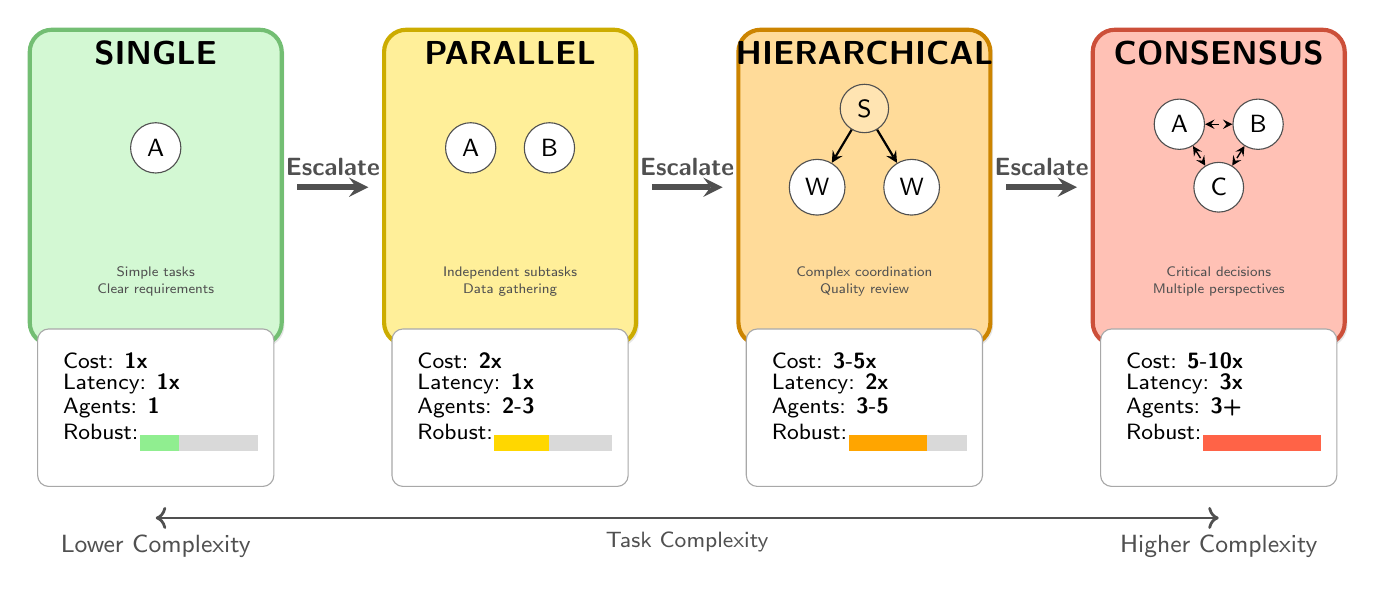
\begin{tikzpicture}[
	patternbox/.style={
		rectangle,
		rounded corners=8pt,
		draw=#1!80!black,
		fill=#1!40,
		line width=1.5pt,
		minimum width=3.2cm,
		minimum height=4cm,
		drop shadow={shadow xshift=1pt, shadow yshift=-1pt, opacity=0.2}
	},
	statsbox/.style={
		rectangle,
		rounded corners=4pt,
		draw=darkgray!50,
		fill=white,
		minimum width=3cm,
		minimum height=2cm,
		font=\sffamily\footnotesize
	},
	arrow/.style={
		->,
		>=stealth,
		line width=2pt,
		color=darkgray
	},
	escalatelabel/.style={
		font=\sffamily\small\bfseries,
		color=darkgray
	},
	agenticon/.style={
		circle,
		draw=darkgray,
		fill=white,
		minimum size=0.6cm,
		font=\sffamily\small
	},
	robustbar/.style={
		rectangle,
		minimum height=0.3cm,
		draw=none
	}
	]
	
	% Title
%	\node[font=\sffamily\Large\bfseries, color=darkgray] at (6.5,5.5) {Escalation Hierarchy with Cost-Robustness Trade-offs};
	
	% Pattern boxes
	\node[patternbox=singlegreen] (single) at (0,2) {};
	\node[patternbox=parallelyellow] (parallel) at (4.5,2) {};
	\node[patternbox=hierarchorange] (hierarchical) at (9,2) {};
	\node[patternbox=consensusred] (consensus) at (13.5,2) {};
	
	% Pattern names
	\node[font=\sffamily\bfseries\large] at (0,3.7) {SINGLE};
	\node[font=\sffamily\bfseries\large] at (4.5,3.7) {PARALLEL};
	\node[font=\sffamily\bfseries\large] at (9,3.7) {HIERARCHICAL};
	\node[font=\sffamily\bfseries\large] at (13.5,3.7) {CONSENSUS};
	
	% Agent icons - Single
	\node[agenticon] at (0,2.5) {A};
	
	% Agent icons - Parallel
	\node[agenticon] at (4,2.5) {A};
	\node[agenticon] at (5,2.5) {B};
	
	% Agent icons - Hierarchical
	\node[agenticon, fill=hierarchorange!30] (hsup) at (9,3) {S};
	\node[agenticon] (hw1) at (8.4,2) {W};
	\node[agenticon] (hw2) at (9.6,2) {W};
	\draw[->, >=stealth, line width=0.8pt] (hsup) -- (hw1);
	\draw[->, >=stealth, line width=0.8pt] (hsup) -- (hw2);
	
	% Agent icons - Consensus
	\node[agenticon] (c1) at (13,2.8) {A};
	\node[agenticon] (c2) at (14,2.8) {B};
	\node[agenticon] (c3) at (13.5,2) {C};
	\draw[<->, >=stealth, line width=0.5pt, dashed] (c1) -- (c2);
	\draw[<->, >=stealth, line width=0.5pt, dashed] (c1) -- (c3);
	\draw[<->, >=stealth, line width=0.5pt, dashed] (c2) -- (c3);
	
	% Stats boxes
	\node[statsbox] (stats1) at (0,-0.8) {};
	\node[statsbox] (stats2) at (4.5,-0.8) {};
	\node[statsbox] (stats3) at (9,-0.8) {};
	\node[statsbox] (stats4) at (13.5,-0.8) {};
	
	% Stats content - Single
	\node[font=\sffamily\footnotesize, anchor=west] at (-1.3,-0.2) {Cost: \textbf{1x}};
	\node[font=\sffamily\footnotesize, anchor=west] at (-1.3,-0.5) {Latency: \textbf{1x}};
	\node[font=\sffamily\footnotesize, anchor=west] at (-1.3,-0.8) {Agents: \textbf{1}};
	\node[font=\sffamily\footnotesize, anchor=west] at (-1.3,-1.1) {Robust:};
	\fill[singlegreen] (-0.2,-1.15) rectangle (0.3,-1.35);
	\fill[gray!30] (0.3,-1.15) rectangle (1.3,-1.35);
	
	% Stats content - Parallel
	\node[font=\sffamily\footnotesize, anchor=west] at (3.2,-0.2) {Cost: \textbf{2x}};
	\node[font=\sffamily\footnotesize, anchor=west] at (3.2,-0.5) {Latency: \textbf{1x}};
	\node[font=\sffamily\footnotesize, anchor=west] at (3.2,-0.8) {Agents: \textbf{2-3}};
	\node[font=\sffamily\footnotesize, anchor=west] at (3.2,-1.1) {Robust:};
	\fill[parallelyellow] (4.3,-1.15) rectangle (5.0,-1.35);
	\fill[gray!30] (5.0,-1.15) rectangle (5.8,-1.35);
	
	% Stats content - Hierarchical
	\node[font=\sffamily\footnotesize, anchor=west] at (7.7,-0.2) {Cost: \textbf{3-5x}};
	\node[font=\sffamily\footnotesize, anchor=west] at (7.7,-0.5) {Latency: \textbf{2x}};
	\node[font=\sffamily\footnotesize, anchor=west] at (7.7,-0.8) {Agents: \textbf{3-5}};
	\node[font=\sffamily\footnotesize, anchor=west] at (7.7,-1.1) {Robust:};
	\fill[hierarchorange] (8.8,-1.15) rectangle (9.8,-1.35);
	\fill[gray!30] (9.8,-1.15) rectangle (10.3,-1.35);
	
	% Stats content - Consensus
	\node[font=\sffamily\footnotesize, anchor=west] at (12.2,-0.2) {Cost: \textbf{5-10x}};
	\node[font=\sffamily\footnotesize, anchor=west] at (12.2,-0.5) {Latency: \textbf{3x}};
	\node[font=\sffamily\footnotesize, anchor=west] at (12.2,-0.8) {Agents: \textbf{3+}};
	\node[font=\sffamily\footnotesize, anchor=west] at (12.2,-1.1) {Robust:};
	\fill[consensusred] (13.3,-1.15) rectangle (14.8,-1.35);
	
	% Escalation arrows
	\draw[arrow] (1.8,2) -- node[above, escalatelabel] {Escalate} (2.7,2);
	\draw[arrow] (6.3,2) -- node[above, escalatelabel] {Escalate} (7.2,2);
	\draw[arrow] (10.8,2) -- node[above, escalatelabel] {Escalate} (11.7,2);
	
	% Complexity scale at bottom
	\draw[<->, line width=1pt, color=darkgray] (0,-2.2) -- (13.5,-2.2);
	\node[font=\sffamily\small, color=darkgray, anchor=north] at (0,-2.3) {Lower Complexity};
	\node[font=\sffamily\small, color=darkgray, anchor=north] at (13.5,-2.3) {Higher Complexity};
	\node[font=\sffamily\footnotesize, color=darkgray] at (6.75,-2.5) {Task Complexity};
	
	% When to use labels
	\node[font=\sffamily\tiny, color=darkgray, text width=2.8cm, align=center] at (0,0.8) {Simple tasks\\Clear requirements};
	\node[font=\sffamily\tiny, color=darkgray, text width=2.8cm, align=center] at (4.5,0.8) {Independent subtasks\\Data gathering};
	\node[font=\sffamily\tiny, color=darkgray, text width=2.8cm, align=center] at (9,0.8) {Complex coordination\\Quality review};
	\node[font=\sffamily\tiny, color=darkgray, text width=2.8cm, align=center] at (13.5,0.8) {Critical decisions\\Multiple perspectives};
	
\end{tikzpicture}
	\caption{Escalation Hierarchy with Cost-Robustness Trade-offs. Shows the four orchestration patterns with their associated costs and robustness levels.}
	\label{fig:framework2}
\end{figure*}

\textbf{Single Pattern:} No communication needed.

\textbf{Parallel Pattern:} Coordinator distributes work, agents work independently, coordinator merges results.

\textbf{Hierarchical Pattern:}
\begin{verbatim}
	Coordinator -> Workers: Task assignment
	Workers -> Coordinator: Progress updates, questions
	Coordinator -> Workers: Guidance, clarifications
	Workers -> Coordinator: Final outputs
	Coordinator: Synthesis and quality check
\end{verbatim}

\textbf{Consensus Pattern:}
\begin{verbatim}
	Round 1: Independent reasoning
	Round 2: Share reasoning, identify disagreements
	Round 3: Deliberation on disagreements
	Round 4: Voting (majority or unanimous based on criticality)
	Round 5: Synthesis of agreed position
\end{verbatim}

\subsection{Budget Management}
\label{sec:budget}

\subsubsection{Cost Model}

Total cost for subtask $t$ with pattern $\pi$:
\begin{equation}
	\text{Cost}(t, \pi) = \sum_{a \in \text{Agents}(\pi)} (c_{\text{input}} \cdot n_{\text{input}}^a + c_{\text{output}} \cdot n_{\text{output}}^a)
\end{equation}
where $c_{\text{input}}$ and $c_{\text{output}}$ are per-token costs for agent $a$'s model.

\subsubsection{Budget Allocation}

Given total budget $B$ and estimated subtask costs:
\begin{equation}
	B_t = B \cdot \frac{\text{EstimatedCost}(t)}{\sum_{t' \in \text{remaining}} \text{EstimatedCost}(t')} \cdot (1 + \delta_{\text{buffer}})
\end{equation}
where $\delta_{\text{buffer}} = 0.1$ reserves capacity for retries/escalations.

\subsubsection{Budget Constraints on Decisions}

When budget is low:
\begin{itemize}
	\item CAR increases single-agent threshold
	\item RCM reduces retry limit
	\item UMA reduces memory retrieval scope
	\item Checkpoints become mandatory only on critical path
\end{itemize}

\subsection{Error Handling and Recovery}
\label{sec:errors}

\subsubsection{Error Categories}

\begin{table}[H]
	\centering
	\caption{Error Handling Strategies}
	\small
	\begin{tabular}{@{}lll@{}}
		\toprule
		\textbf{Error Type} & \textbf{Detection} & \textbf{Recovery} \\
		\midrule
		API timeout & HTTP status & Retry with backoff \\
		Rate limit & HTTP 429 & Queue and wait \\
		Context overflow & Token count & Compress context \\
		Tool failure & Tool output & Alternative tool or manual \\
		Quality failure & RCM checkpoint & Retry/escalate/replan \\
		Budget exhaustion & Cost tracking & Graceful degradation \\
		\bottomrule
	\end{tabular}
\end{table}

\subsubsection{Graceful Degradation}

When recovery is impossible:
\begin{enumerate}
	\item Mark subtask as failed with partial output
	\item Assess impact on downstream subtasks
	\item Attempt to continue with degraded quality
	\item Report failure to user with explanation
\end{enumerate}

\section{Detailed Algorithms}
\label{app:algorithms}

\subsection{Algorithm A1: Complexity-Aware Routing}

\begin{algorithm}[H]
	\caption{Complexity-Aware Routing (\car{})}
	\label{alg:car_detailed}
	\begin{algorithmic}[1]
		\REQUIRE Task $\mathcal{T}$, Budget $B$, Agent Pool $\mathcal{A}$, History $\mathcal{H}$
		\ENSURE Execution Plan $P$
		
		\STATE $D \leftarrow \text{InitialDecompose}(\mathcal{T})$ \COMMENT{Task decomposition}
		\STATE $G \leftarrow \text{BuildDependencyGraph}(D)$
		\STATE $P \leftarrow []$
		\STATE $B_{\text{remaining}} \leftarrow B$
		
		\FOR{$t$ in $\text{TopologicalSort}(G)$}
		\STATE \COMMENT{Extract features for subtask}
		\STATE $f_{\text{length}} \leftarrow \text{EstimateReasoningSteps}(t, \mathcal{H})$
		\STATE $f_{\text{tools}} \leftarrow |\text{RequiredTools}(t)| / 10$
		\STATE $f_{\text{knowledge}} \leftarrow \text{DomainBreadth}(t)$
		\STATE $f_{\text{ambiguity}} \leftarrow \text{SemanticEntropy}(t)$
		\STATE $f_{\text{deps}} \leftarrow |\text{Predecessors}(G, t)| / |D|$
		\STATE $f_{\text{critical}} \leftarrow \mathbb{1}[\text{OnCriticalPath}(G, t)]$
		\STATE $f_{\text{history}} \leftarrow \text{LookupHistoricalSuccess}(t, \mathcal{H})$
		
		\STATE $\mathbf{x}_t \leftarrow [f_{\text{length}}, f_{\text{tools}}, f_{\text{knowledge}}, f_{\text{ambiguity}}, f_{\text{deps}}, f_{\text{critical}}, f_{\text{history}}]$
		
		\STATE \COMMENT{Predict pattern distribution}
		\STATE $\pi_{\text{dist}} \leftarrow \text{softmax}(W_\pi \cdot \text{MLP}(\mathbf{x}_t))$
		
		\STATE \COMMENT{Dynamic threshold adaptation}
		\STATE $\tau \leftarrow \tau_0 + \lambda \cdot (B_{\text{remaining}} / B)$
		
		\IF{$\pi_{\text{dist}}[\text{single}] > \tau$}
		\STATE $\pi \leftarrow \text{SINGLE}$
		\ELSE
		\STATE $\pi \leftarrow \arg\max_{\pi' \neq \text{single}} \pi_{\text{dist}}[\pi']$
		\ENDIF
		
		\STATE $\text{agents} \leftarrow \text{SelectAgents}(t, \pi, \mathcal{A})$
		\STATE $P.\text{append}((t, \pi, \text{agents}))$
		\STATE $B_{\text{remaining}} \leftarrow B_{\text{remaining}} - \text{EstimateCost}(t, \pi, \text{agents})$
		\ENDFOR
		
		\STATE \textbf{return} $P$
	\end{algorithmic}
\end{algorithm}

\subsection{Algorithm A2: Reflective Checkpoint}

\begin{algorithm}[H]
	\caption{Reflective Checkpoint Mechanism (\rcm{})}
	\label{alg:rcm_detailed}
	\begin{algorithmic}[1]
		\REQUIRE Output $o_t$, Subtask $t$, Pattern $\pi$, Context $C$, Thresholds $\theta_{\text{high}}, \theta_{\text{low}}$
		\ENSURE Action, Updated Plan (optional)
		
		\STATE \COMMENT{Assess quality across three dimensions}
		\STATE $Q_{\text{complete}} \leftarrow \text{LLMJudge}(o_t, t, \text{``completeness''})$
		\STATE $Q_{\text{coherent}} \leftarrow \text{EntailmentCheck}(o_t) \cdot \text{ContradictionScore}(o_t)$
		\STATE $Q_{\text{useful}} \leftarrow \text{ForwardSimulation}(o_t, \text{DownstreamTasks}(t))$
		
		\STATE $Q \leftarrow \lambda_1 Q_{\text{complete}} + \lambda_2 Q_{\text{coherent}} + \lambda_3 Q_{\text{useful}}$
		
		\STATE \COMMENT{Check for structural issues}
		\STATE $\text{structural\_issue} \leftarrow \text{DetectMissingSubtask}(o_t, C) \lor \text{DetectWrongDeps}(o_t, C)$
		
		\IF{$\text{structural\_issue}$}
		\STATE $\text{reflection} \leftarrow \text{LLMReflect}(o_t, t, \text{RemainingTasks})$
		\STATE $\text{new\_plan} \leftarrow \text{Replan}(\text{reflection}, \text{RemainingTasks})$
		\STATE \textbf{return} \textsc{Replan}, $\text{new\_plan}$
		\ENDIF
		
		\IF{$Q \geq \theta_{\text{high}}$}
		\STATE \textbf{return} \textsc{Proceed}, None
		\ENDIF
		
		\IF{$Q \geq \theta_{\text{low}}$}
		\IF{$C.\text{retries} < \text{MAX\_RETRIES}$}
		\STATE \textbf{return} \textsc{Retry}, None
		\ELSIF{$C.\text{escalations} < \text{MAX\_ESCALATIONS}$}
		\STATE $\pi_{\text{new}} \leftarrow \text{Escalate}(\pi)$
		\STATE \textbf{return} \textsc{Escalate}, $(t, \pi_{\text{new}})$
		\ELSE
		\STATE \textbf{return} \textsc{Proceed}, None \COMMENT{Accept lower quality}
		\ENDIF
		\ENDIF
		
		\STATE \COMMENT{Quality below $\theta_{\text{low}}$}
		\IF{$C.\text{escalations} < \text{MAX\_ESCALATIONS}$}
		\STATE $\pi_{\text{new}} \leftarrow \text{Escalate}(\pi)$
		\STATE \textbf{return}
		\STATE $\text{reflection} \leftarrow \text{LLMReflect}(o_t, t, \text{RemainingTasks})$
		\STATE $\text{new\_plan} \leftarrow \text{Replan}(\text{reflection}, \text{RemainingTasks})$
		\STATE \textbf{return} \textsc{Replan}, $\text{new\_plan}$
		\ENDIF
		
	\end{algorithmic}
\end{algorithm}

\subsection{Algorithm A3: Memory Consolidation}

\begin{algorithm}[H]
	\caption{Unified Memory Consolidation (\uma{})}
	\label{alg:uma_detailed}
	\begin{algorithmic}[1]
		\REQUIRE Episodic Store $M_E$, Semantic Store $M_S$, Threshold $\tau$
		\ENSURE Updated Semantic Store $M_S$
		
		\FOR{$\text{episode}$ in $M_E.\text{GetRecent}()$}
		\STATE \COMMENT{Extract key facts from episode}
		\STATE $\text{facts} \leftarrow \text{LLMExtractFacts}(\text{episode.trace})$
		
		\FOR{$\text{fact}$ in $\text{facts}$}
		\STATE \COMMENT{Compute importance based on success and frequency}
		\STATE $\text{importance} \leftarrow \alpha \cdot \text{episode.success} + \beta \cdot \text{Frequency}(\text{fact}, M_E)$
		
		\IF{$\text{importance} > \tau$}
		\STATE \COMMENT{Check for duplicates using embedding similarity}
		\STATE $\text{similar} \leftarrow M_S.\text{FindSimilar}(\text{fact}, \text{threshold}=0.9)$
		
		\IF{$|\text{similar}| = 0$}
		\STATE \COMMENT{Add new fact to knowledge graph}
		\STATE $\text{entities} \leftarrow \text{ExtractEntities}(\text{fact})$
		\STATE $\text{relations} \leftarrow \text{ExtractRelations}(\text{fact})$
		\STATE $M_S.\text{AddToGraph}(\text{entities}, \text{relations})$
		\STATE $M_S.\text{AddEmbedding}(\text{fact})$
		\ELSE
		\STATE \COMMENT{Update existing fact with new evidence}
		\STATE $M_S.\text{UpdateConfidence}(\text{similar}[0], \text{importance})$
		\ENDIF
		\ENDIF
		\ENDFOR
		
		\STATE \COMMENT{Archive processed episode}
		\STATE $M_E.\text{Archive}(\text{episode})$
		\ENDFOR
		
		\STATE \textbf{return} $M_S$
	\end{algorithmic}
\end{algorithm}

% ==============================================================================
% B. MARS BENCHMARK SPECIFICATION
% ==============================================================================
\section{\mars{} Benchmark Specification}
\label{app:mars}

\subsection{Task Schema}

Each task in \mars{} follows this JSON schema:

\begin{lstlisting}[language=json, basicstyle=\small\ttfamily]
	{
		"id": "string",
		"category": "scientific_research|software_engineering|strategic_planning",
		"description": "string",
		"complexity_level": "low|medium_low|medium|medium_high|high",
		"subtasks": [
		{
			"id": "string",
			"description": "string",
			"complexity": 0.0-1.0,
			"required_tools": ["tool_names"],
			"dependencies": ["subtask_ids"],
			"optimal_pattern": "single|parallel|hierarchical|consensus",
			"estimated_steps": integer,
			"evaluation_criteria": {
				"completeness": "rubric",
				"correctness": "rubric",
				"efficiency": "rubric"
			}
		}
		],
		"ground_truth": {
			"final_answer": "string or structured",
			"key_insights": ["strings"],
			"required_tool_calls": [{"tool": "name", "args": {...}}]
		},
		"metadata": {
			"domain": "string",
			"difficulty_rating": 1-5,
			"estimated_time_minutes": integer,
			"annotator_id": "string",
			"annotation_date": "ISO date"
		}
	}
\end{lstlisting}

\subsection{Task Category Details}

\subsubsection{Scientific Research (847 tasks)}

\textbf{Domains:} Biology (284), Physics (198), Computer Science (212), Chemistry (153)

\textbf{Task Types:}
\begin{itemize}[nosep]
	\item Literature Review (35\%): Synthesize research on a specific topic
	\item Methodology Analysis (25\%): Evaluate experimental approaches
	\item Gap Identification (20\%): Find unexplored research directions
	\item Hypothesis Generation (20\%): Propose testable hypotheses
\end{itemize}

\textbf{Example Task:}
\begin{quote}
	\textit{``Conduct a systematic review of transformer efficiency techniques published since 2022. Identify the top 5 approaches by computational savings, analyze their trade-offs, and propose a novel combination that could achieve better results.''}
\end{quote}

\textbf{Optimal Pattern Distribution:}
\begin{itemize}[nosep]
	\item Paper retrieval: Parallel (multiple databases)
	\item Individual paper analysis: Single agent
	\item Cross-paper synthesis: Hierarchical (coordinator + analysts)
	\item Novel proposal generation: Consensus (multiple perspectives)
\end{itemize}

\subsubsection{Software Engineering (1,124 tasks)}

\textbf{Domains:} Web Development (412), Systems Programming (298), ML Engineering (248), DevOps (166)

\textbf{Task Types:}
\begin{itemize}[nosep]
	\item Bug Localization \& Fix (30\%): Identify and resolve issues
	\item Code Review (25\%): Evaluate code quality and suggest improvements
	\item Feature Implementation (25\%): Add new functionality
	\item Test Generation (20\%): Create comprehensive test suites
\end{itemize}

\textbf{Example Task:}
\begin{quote}
	\textit{``Debug the performance regression in the authentication module that appeared after commit abc123. Identify the root cause, implement a fix, write regression tests, and ensure backward compatibility.''}
\end{quote}

\subsubsection{Strategic Planning (876 tasks)}

\textbf{Domains:} Business Strategy (324), Policy Analysis (287), Product Design (265)

\textbf{Task Types:}
\begin{itemize}[nosep]
	\item Market Analysis (30\%): Evaluate competitive landscape
	\item Decision Synthesis (25\%): Integrate multiple factors for recommendations
	\item Risk Assessment (25\%): Identify and evaluate potential risks
	\item Scenario Planning (20\%): Develop contingency strategies
\end{itemize}

\subsection{Annotation Process}
\label{sub:ann}

\textbf{Phase 1: Task Creation}
\begin{enumerate}[nosep]
	\item Domain experts created initial tasks based on real-world scenarios
	\item Tasks were reviewed for clarity and completeness
	\item Subtask decomposition was performed by experienced annotators
\end{enumerate}

\textbf{Phase 2: Pattern Labeling}
\begin{enumerate}[nosep]
	\item Three annotators independently labeled optimal patterns for each subtask
	\item Inter-annotator agreement: Cohen's $\kappa = 0.78$
	\item Disagreements resolved through discussion and empirical validation
\end{enumerate}

\textbf{Phase 3: Validation}
\begin{enumerate}[nosep]
	\item Subset (10\%) executed with different patterns to validate labels
	\item Ground truth answers verified by domain experts
	\item Quality control: 5\% of tasks randomly re-annotated monthly
\end{enumerate}

\subsection{Evaluation Protocol}

\textbf{Task Success Criteria:}
\begin{itemize}[nosep]
	\item Binary success: Task achieves $\geq$80\% subtask completion
	\item Subtask success: Output meets completeness, correctness, efficiency criteria
	\item Partial credit: Weighted by subtask importance
\end{itemize}

\textbf{Orchestration Metrics:}
\begin{itemize}[nosep]
	\item Orchestration Accuracy = $\frac{\text{Correct patterns}}{\text{Total subtasks}}$
	\item Adaptation Rate = $\frac{\text{Successful adaptations}}{\text{Adaptation attempts}}$
	\item Memory Utilization = $\frac{\text{Used retrieved memories}}{\text{Total retrieved}}$
\end{itemize}

% ==============================================================================
% C. ADDITIONAL EXPERIMENTAL RESULTS
% ==============================================================================
\section{Additional Experimental Results}
\label{app:results}

\subsection{Per-Domain \mars{} Results}

\begin{table}[H]
	\caption{Detailed \mars{} Results by Domain}
	\centering
	\small
	\begin{tabular}{@{}lcccc@{}}
		\toprule
		\textbf{Domain} & \textbf{\amore{}} & \textbf{AgentOrch.} & \textbf{Single} & \textbf{$\Delta$ Best} \\
		\midrule
		\multicolumn{5}{c}{\textit{Scientific Research}} \\
		\midrule
		Biology & 54.2 & 45.1 & 31.8 & +9.1 \\
		Physics & 48.7 & 41.3 & 28.4 & +7.4 \\
		Computer Science & 53.4 & 44.2 & 33.1 & +9.2 \\
		Chemistry & 50.1 & 42.8 & 29.7 & +7.3 \\
		\midrule
		\multicolumn{5}{c}{\textit{Software Engineering}} \\
		\midrule
		Web Development & 61.2 & 52.4 & 41.2 & +8.8 \\
		Systems Programming & 55.8 & 48.7 & 36.5 & +7.1 \\
		ML Engineering & 58.2 & 49.1 & 38.8 & +9.1 \\
		DevOps & 56.4 & 50.2 & 37.4 & +6.2 \\
		\midrule
		\multicolumn{5}{c}{\textit{Strategic Planning}} \\
		\midrule
		Business Strategy & 44.1 & 35.8 & 23.1 & +8.3 \\
		Policy Analysis & 42.8 & 34.2 & 21.5 & +8.6 \\
		Product Design & 48.7 & 40.5 & 29.8 & +8.2 \\
		\bottomrule
	\end{tabular}
\end{table}


\subsection{Scalability Analysis}
\begin{figure*}[t]
	\centering
	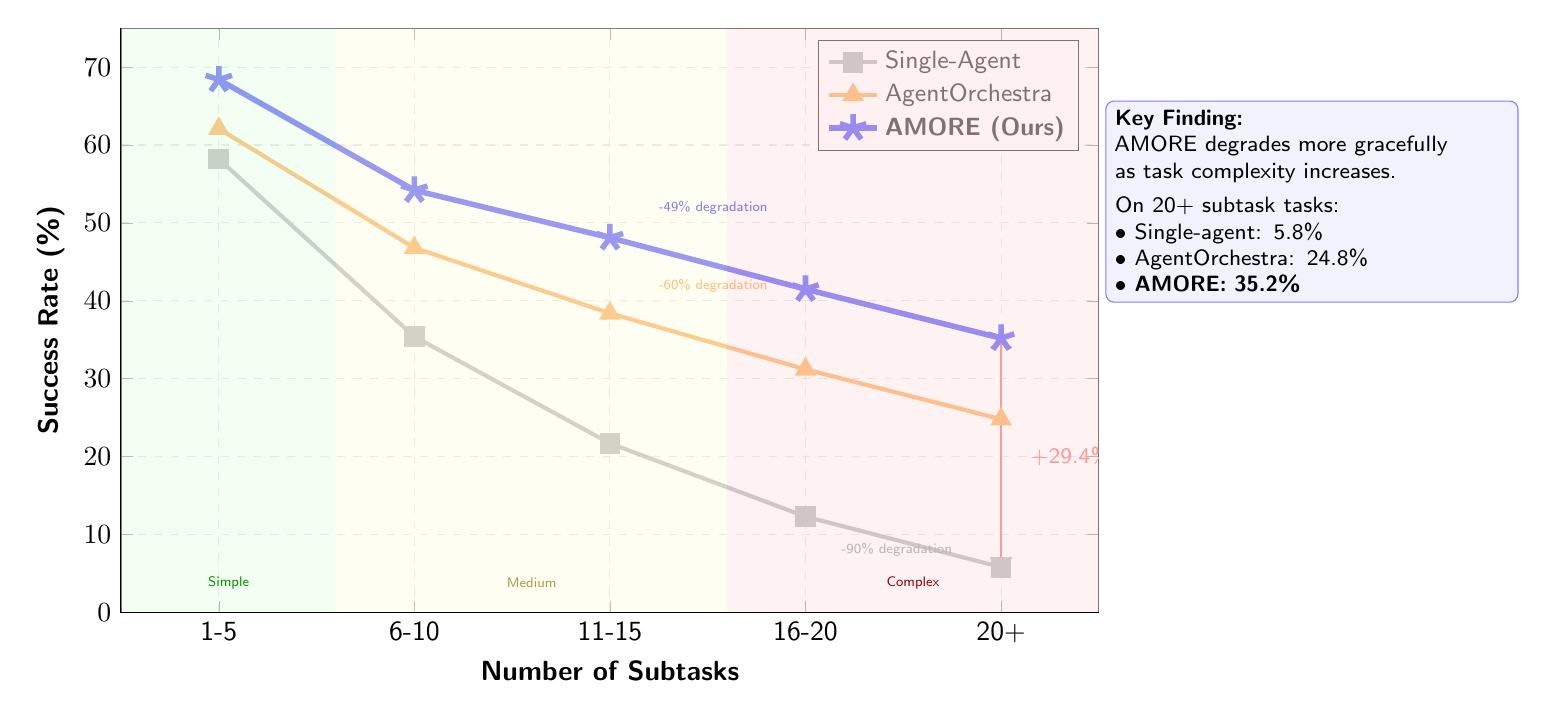
\begin{tikzpicture}
	\begin{axis}[
		width=14cm,
		height=9cm,
		xlabel={\textbf{Number of Subtasks}},
		ylabel={\textbf{Success Rate (\%)}},
		xmin=0.5,
		xmax=5.5,
		ymin=0,
		ymax=75,
		xtick={1,2,3,4,5},
		xticklabels={1-5, 6-10, 11-15, 16-20, 20+},
		ytick={0,10,20,30,40,50,60,70},
		grid=both,
		grid style={dashed, gray!30},
		ylabel style={font=\sffamily\bfseries},
		xlabel style={font=\sffamily\bfseries},
		tick label style={font=\sffamily},
%		title={\sffamily\bfseries\large Performance vs. Task Complexity (Number of Subtasks)},
		title style={yshift=8pt},
		legend style={
			at={(0.98,0.98)},
			anchor=north east,
			font=\sffamily\small,
			cells={anchor=west}
		}
		]
		% Single-Agent baseline
		\addplot[
		color=gray!70,
		mark=square*,
		mark size=3pt,
		line width=1.5pt
		] coordinates {
			(1, 58.2)
			(2, 35.4)
			(3, 21.7)
			(4, 12.3)
			(5, 5.8)
		};
		% AgentOrchestra
		\addplot[
		color=orange!80,
		mark=triangle*,
		mark size=3pt,
		line width=1.5pt
		] coordinates {
			(1, 62.1)
			(2, 46.8)
			(3, 38.4)
			(4, 31.2)
			(5, 24.8)
		};
		% AMORE
		\addplot[
		color=blue!80,
		mark=star,
		mark size=5pt,
		line width=2pt
		] coordinates {
			(1, 68.4)
			(2, 54.2)
			(3, 48.1)
			(4, 41.5)
			(5, 35.2)
		};
		\legend{Single-Agent, AgentOrchestra, \textbf{AMORE (Ours)}}
		% Annotations for key differences
		% Gap annotation at complex tasks
		\draw[<->, line width=1pt, color=red!70] (axis cs:5,5.8) -- (axis cs:5,35.2);
		\node[font=\sffamily\footnotesize, color=red!70, anchor=west] at (axis cs:5.1,20) {+29.4\%};
		% Degradation rates
		\node[font=\sffamily\tiny, color=gray, anchor=east, text width=2.5cm, align=right] at (axis cs:4.8,8) {-90\% degradation};
		\node[font=\sffamily\tiny, color=orange, anchor=west] at (axis cs:3.2,42) {-60\% degradation};
		\node[font=\sffamily\tiny, color=blue, anchor=west] at (axis cs:3.2,52) {-49\% degradation};
	\end{axis}
	% Insight box
	\node[draw=blue!50, fill=blue!5, rounded corners=3pt, font=\sffamily\footnotesize, text width=5cm, align=left, anchor=north west] at (12.5,6.5) {
		\textbf{Key Finding:}\\
		AMORE degrades more gracefully\\
		as task complexity increases.\\[3pt]
		On 20+ subtask tasks:\\
		\textbullet\ Single-agent: 5.8\%\\
		\textbullet\ AgentOrchestra: 24.8\%\\
		\textbullet\ \textbf{AMORE: 35.2\%}
	};
	% Complexity zone annotations
	\fill[green!10, opacity=0.5] (rel axis cs:0,0) rectangle (rel axis cs:0.22,1);
	\fill[yellow!10, opacity=0.5] (rel axis cs:0.22,0) rectangle (rel axis cs:0.62,1);
	\fill[red!10, opacity=0.5] (rel axis cs:0.62,0) rectangle (rel axis cs:1,1);
	\node[font=\sffamily\tiny, color=green!60!black] at (rel axis cs:0.11,0.05) {Simple};
	\node[font=\sffamily\tiny, color=yellow!60!black] at (rel axis cs:0.42,0.05) {Medium};
	\node[font=\sffamily\tiny, color=red!60!black] at (rel axis cs:0.81,0.05) {Complex};
\end{tikzpicture}
	\caption{ Performance vs. Task Complexity (Number of Subtasks)}
	\label{fig:framework9}
\end{figure*}

\begin{table}[H]
	\caption{Performance vs. Number of Subtasks}
	\centering
	\small
	\begin{tabular}{@{}lccccc@{}}
		\toprule
		\textbf{Subtasks} & \textbf{\amore{}} & \textbf{AgentOrch.} & \textbf{HALO} & \textbf{MetaGPT} & \textbf{Single} \\
		\midrule
		1-5 & 68.4 & 62.1 & 59.8 & 56.2 & 58.2 \\
		6-10 & 54.2 & 46.8 & 44.1 & 41.5 & 35.4 \\
		11-15 & 48.1 & 38.4 & 35.2 & 32.8 & 21.7 \\
		16-20 & 41.5 & 31.2 & 27.5 & 24.1 & 12.3 \\
		20+ & 35.2 & 24.8 & 20.1 & 17.2 & 5.8 \\
		\midrule
		\textit{Degradation} & -49\% & -60\% & -66\% & -69\% & -90\% \\
		\bottomrule
	\end{tabular}
\end{table}

\subsection{Pattern Selection Analysis}

\begin{table}[H]
	\caption{\car{} Pattern Prediction Accuracy by Complexity}
	\centering
	\small
	\begin{tabular}{@{}lccccc@{}}
		\toprule
		\textbf{Complexity} & \textbf{Overall} & \textbf{Single} & \textbf{Parallel} & \textbf{Hier.} & \textbf{Cons.} \\
		\midrule
		Low & 92.4\% & 94.1\% & 88.2\% & 85.3\% & 78.1\% \\
		Medium-Low & 89.7\% & 91.2\% & 89.5\% & 87.4\% & 82.3\% \\
		Medium & 87.2\% & 85.4\% & 88.1\% & 88.7\% & 85.6\% \\
		Medium-High & 85.8\% & 81.2\% & 84.3\% & 89.2\% & 88.1\% \\
		High & 83.1\% & 75.4\% & 78.6\% & 86.8\% & 91.2\% \\
		\midrule
		\textbf{Average} & \textbf{88.3\%} & 85.5\% & 85.7\% & 87.5\% & 85.1\% \\
		\bottomrule
	\end{tabular}
\end{table}

\subsection{Cost-Performance Detailed Analysis}

\begin{table}[H]
	\caption{Detailed Cost Analysis (Cost per Task in \$)}
	\centering
	\small
	\begin{tabular}{@{}lcccccc@{}}
		\toprule
		\textbf{Method} & \textbf{Sci.} & \textbf{SWE} & \textbf{Strat.} & \textbf{Avg} & \textbf{Succ/\$} \\
		\midrule
		GPT-4 + ReAct & 2.45 & 1.87 & 2.10 & 2.14 & 15.0 \\
		AutoGen & 4.21 & 3.52 & 3.82 & 3.85 & 9.4 \\
		MetaGPT & 4.58 & 3.91 & 4.14 & 4.21 & 9.3 \\
		HALO & 5.67 & 4.78 & 4.91 & 5.12 & 8.2 \\
		AgentOrchestra & 7.12 & 5.98 & 6.31 & 6.47 & 6.8 \\
		\textbf{\amore{}} & \textbf{4.15} & \textbf{3.41} & \textbf{3.90} & \textbf{3.82} & \textbf{13.7} \\
		\bottomrule
	\end{tabular}
\end{table}

\subsection{\rcm{} Checkpoint Statistics}

\begin{table}[H]
	\caption{Checkpoint Action Distribution}
	\centering
	\small
	\begin{tabular}{@{}lcccc@{}}
		\toprule
		\textbf{Action} & \textbf{Frequency} & \textbf{Success After} & \textbf{Avg Cost} \\
		\midrule
		Proceed & 71.2\% & N/A & 1.0$\times$ \\
		Retry & 14.8\% & 68.4\% & 1.8$\times$ \\
		Escalate & 10.3\% & 72.1\% & 2.5$\times$ \\
		Replan & 3.7\% & 54.2\% & 3.2$\times$ \\
		\bottomrule
	\end{tabular}
\end{table}

\subsection{\uma{} Memory Statistics}

\begin{figure*}[t]
	\centering
	\definecolor{workingblue}{RGB}{70,130,180}
\definecolor{episodicgreen}{RGB}{60,179,113}
\definecolor{semanticpurple}{RGB}{147,112,219}
\definecolor{agentcolor}{RGB}{255,165,0}

\begin{tikzpicture}[
	tier/.style={
		rectangle,
		rounded corners=5pt,
		draw=#1!80!black,
		fill=#1!15,
		line width=1.5pt,
		minimum width=14cm,
		drop shadow={shadow xshift=1pt, shadow yshift=-1pt, opacity=0.2}
	},
	agentbox/.style={
		rectangle,
		rounded corners=3pt,
		draw=agentcolor!80!black,
		fill=agentcolor!20,
		minimum width=2.5cm,
		minimum height=2cm,
		font=\sffamily\small
	},
	memoryitem/.style={
		rectangle,
		rounded corners=2pt,
		draw=darkgray!50,
		fill=white,
		minimum width=3.5cm,
		minimum height=1.5cm,
		font=\sffamily\footnotesize
	},
	arrow/.style={
		->,
		>=stealth,
		line width=1.2pt,
		color=darkgray
	},
	syncarrow/.style={
		->,
		>=stealth,
		line width=1pt,
		color=#1,
		dashed
	},
	tierlabel/.style={
		font=\sffamily\bfseries\large,
		color=#1!80!black
	},
	sublabel/.style={
		font=\sffamily\footnotesize,
		color=darkgray
	}
	]
	
	% Main title
	%\node[font=\sffamily\Large\bfseries, color=darkgray] at (0,9) {Unified Memory Architecture (UMA)};
	
	% === WORKING MEMORY TIER ===
	\node[tier=workingblue, minimum height=3cm] (working) at (0,6.5) {};
	\node[tierlabel=workingblue, anchor=west] at (-6.5,7.7) {WORKING MEMORY ($M_W$)};
	\node[sublabel, anchor=west] at (-6.5,7.3) {Per-Agent, Immediate Access, Limited Capacity (~100K tokens)};
	
	% Agent boxes in working memory
	\node[agentbox] (agent1) at (-4.5,5.8) {};
	\node[font=\sffamily\bfseries\small] at (-4.5,6.4) {Agent 1};
	\node[font=\sffamily\tiny, text width=2cm, align=center] at (-4.5,5.6) {Context\\Goals\\Outputs};
	
	\node[agentbox] (agent2) at (-1.5,5.8) {};
	\node[font=\sffamily\bfseries\small] at (-1.5,6.4) {Agent 2};
	\node[font=\sffamily\tiny, text width=2cm, align=center] at (-1.5,5.6) {Context\\Goals\\Outputs};
	
	\node[agentbox] (agent3) at (1.5,5.8) {};
	\node[font=\sffamily\bfseries\small] at (1.5,6.4) {Agent 3};
	\node[font=\sffamily\tiny, text width=2cm, align=center] at (1.5,5.6) {Context\\Goals\\Outputs};
	
	\node[font=\sffamily\large] at (4,5.8) {...};
	
	\node[agentbox] (agentn) at (5.5,5.8) {};
	\node[font=\sffamily\bfseries\small] at (5.5,6.4) {Agent N};
	\node[font=\sffamily\tiny, text width=2cm, align=center] at (5.5,5.6) {Context\\Goals\\Outputs};
	
	% === EPISODIC MEMORY TIER ===
	\node[tier=episodicgreen, minimum height=2.8cm] (episodic) at (0,3) {};
	\node[tierlabel=episodicgreen, anchor=west] at (-6.5,4.1) {EPISODIC MEMORY ($M_E$)};
	\node[sublabel, anchor=west] at (-6.5,3.7) {Session-Level, RAG Retrieval, ~10M entries};
	
	% Memory items in episodic
	\node[memoryitem] (traces) at (-4,2.5) {};
	\node[font=\sffamily\footnotesize\bfseries] at (-4,3) {Execution Traces};
	\node[font=\sffamily\tiny, text width=3cm, align=center] at (-4,2.3) {trace\_001: \{...\}\\trace\_002: \{...\}};
	
	\node[memoryitem] (patterns) at (0,2.5) {};
	\node[font=\sffamily\footnotesize\bfseries] at (0,3) {Success Patterns};
	\node[font=\sffamily\tiny, text width=3cm, align=center] at (0,2.3) {pattern\_A: \{...\}\\pattern\_B: \{...\}};
	
	\node[memoryitem] (failures) at (4,2.5) {};
	\node[font=\sffamily\footnotesize\bfseries] at (4,3) {Failure Cases};
	\node[font=\sffamily\tiny, text width=3cm, align=center] at (4,2.3) {failure\_X: \{...\}\\failure\_Y: \{...\}};
	
	% === SEMANTIC MEMORY TIER ===
	\node[tier=semanticpurple, minimum height=3.2cm] (semantic) at (0,-0.8) {};
	\node[tierlabel=semanticpurple, anchor=west] at (-6.5,0.5) {SEMANTIC MEMORY ($M_S$)};
	\node[sublabel, anchor=west] at (-6.5,0.1) {Permanent, Knowledge Graph + Embeddings, Unlimited};
	
	% Knowledge items in semantic
	\node[memoryitem, minimum width=3cm] (domain) at (-4,-1.3) {};
	\node[font=\sffamily\footnotesize\bfseries] at (-4,-0.8) {Domain Knowledge};
	\node[font=\sffamily\tiny] at (-4,-1.5) {Facts, concepts, rules};
	
	\node[memoryitem, minimum width=3cm] (strategies) at (0,-1.3) {};
	\node[font=\sffamily\footnotesize\bfseries] at (0,-0.8) {Learned Strategies};
	\node[font=\sffamily\tiny] at (0,-1.5) {Effective approaches};
	
	\node[memoryitem, minimum width=3cm] (insights) at (4,-1.3) {};
	\node[font=\sffamily\footnotesize\bfseries] at (4,-0.8) {Persistent Insights};
	\node[font=\sffamily\tiny] at (4,-1.5) {Cross-session learning};
	
	% Knowledge graph visualization
	\node[circle, draw=semanticpurple, fill=semanticpurple!30, minimum size=0.4cm] (n1) at (-2.5,-2.3) {};
	\node[circle, draw=semanticpurple, fill=semanticpurple!30, minimum size=0.4cm] (n2) at (-1.5,-2.3) {};
	\node[circle, draw=semanticpurple, fill=semanticpurple!30, minimum size=0.4cm] (n3) at (-2,-2.8) {};
	\draw[-, semanticpurple, line width=0.8pt] (n1) -- (n2);
	\draw[-, semanticpurple, line width=0.8pt] (n1) -- (n3);
	\draw[-, semanticpurple, line width=0.8pt] (n2) -- (n3);
	\node[font=\sffamily\tiny, color=semanticpurple] at (-2,-3.2) {Knowledge Graph};
	
	% Vector space visualization
	\node[font=\sffamily\tiny, color=semanticpurple] at (2,-2.2) {$\vec{e}_1$};
	\node[font=\sffamily\tiny, color=semanticpurple] at (2.5,-2.5) {$\vec{e}_2$};
	\node[font=\sffamily\tiny, color=semanticpurple] at (1.8,-2.7) {$\vec{e}_3$};
	\draw[->, semanticpurple, line width=0.5pt] (1.5,-2.5) -- (2,-2.2);
	\draw[->, semanticpurple, line width=0.5pt] (1.5,-2.5) -- (2.5,-2.5);
	\draw[->, semanticpurple, line width=0.5pt] (1.5,-2.5) -- (1.8,-2.7);
	\node[font=\sffamily\tiny, color=semanticpurple] at (2,-3.2) {Embeddings};
	
	% === ARROWS BETWEEN TIERS ===
	
	% Sync arrows from agents to episodic
	\draw[syncarrow=workingblue] (agent1.south) -- ++(0,-0.5) -- ++(-0.5,0) |- (traces.north west);
	\draw[syncarrow=workingblue] (agent2.south) -- (patterns.north);
	\draw[syncarrow=workingblue] (agent3.south) -- ++(0,-0.5) -- ++(1,0) |- (failures.north west);
	
	% Sync label
	\node[font=\sffamily\footnotesize\bfseries, color=workingblue, rotate=90] at (-6.8,4.7) {Sync \& Share};
	
	% Consolidation arrow
	\draw[arrow, line width=2pt, color=episodicgreen] (0,1.5) -- node[right, font=\sffamily\footnotesize, color=darkgray] {Consolidation} node[right, font=\sffamily\tiny, color=darkgray, yshift=-0.3cm] {(importance $> \tau$)} (0,0.6);
	
	% Retrieval arrows (going up)
	\draw[arrow, line width=1pt, color=semanticpurple, dashed] (-5.5,-0.5) -- (-5.5,5);
	\node[font=\sffamily\tiny, color=semanticpurple, rotate=90] at (-5.8,2.5) {Retrieval (RAG)};
	
	% Cross-agent sharing indicator
	\draw[<->, line width=1pt, color=agentcolor, dashed] (agent1.east) -- (agent2.west);
	\draw[<->, line width=1pt, color=agentcolor, dashed] (agent2.east) -- (agent3.west);
	\node[font=\sffamily\tiny, color=agentcolor] at (-3,7.2) {Cross-agent sync};
	
	% Persistence labels on right
	\node[font=\sffamily\footnotesize, color=workingblue, anchor=west] at (7,6.5) {Persistence: Subtask};
	\node[font=\sffamily\footnotesize, color=episodicgreen, anchor=west] at (7,3) {Persistence: Session};
	\node[font=\sffamily\footnotesize, color=semanticpurple, anchor=west] at (7,-0.8) {Persistence: Permanent};
	
\end{tikzpicture}
	\caption{Unified Memory Architecture (UMA). Three-tier memory system showing how agents share and consolidate memory.}
	\label{fig:framework3}
\end{figure*}


\begin{table}[H]
	\caption{Memory Utilization Across Task Types}
	\centering
	\small
	\begin{tabular}{@{}lcccc@{}}
		\toprule
		\textbf{Category} & \textbf{Working} & \textbf{Episodic} & \textbf{Semantic} & \textbf{Consol. Rate} \\
		\midrule
		Scientific & 45.2K & 128.4K & 23.1K & 18.0\% \\
		Software & 38.7K & 95.2K & 31.4K & 33.0\% \\
		Strategic & 52.1K & 156.8K & 28.7K & 18.3\% \\
		\midrule
		\textbf{Average} & 45.3K & 126.8K & 27.7K & 21.8\% \\
		\bottomrule
	\end{tabular}
\end{table}



% ==============================================================================
% D. IMPLEMENTATION DETAILS
% ==============================================================================
\section{Implementation Details}
\label{app:implementation}

\subsection{Model Configuration}

\begin{table}[H]
	\caption{Model Configuration}
	\centering
	\small
	\begin{tabular}{@{}ll@{}}
		\toprule
		\textbf{Component} & \textbf{Configuration} \\
		\midrule
		Coordinator LLM & GPT-4-Turbo (gpt-4-1106-preview) \\
		Worker LLM & GPT-3.5-Turbo (gpt-3.5-turbo-1106) \\
		Quality Judge & GPT-4 (for LLM-as-judge) \\
		\car{} MLP & 3 layers, 256 hidden units, ReLU \\
		Episodic Memory & ChromaDB with OpenAI embeddings \\
		Semantic Memory & Neo4j + text-embedding-3-small \\
		\bottomrule
	\end{tabular}
\end{table}

\subsection{Hyperparameters}

\begin{table}[H]
	\caption{Hyperparameter Settings}
	\centering
	\small
	\begin{tabular}{@{}lcc@{}}
		\toprule
		\textbf{Parameter} & \textbf{Value} & \textbf{Tuning Range} \\
		\midrule
		$\theta_{\text{high}}$ & 0.80 & [0.70, 0.90] \\
		$\theta_{\text{low}}$ & 0.50 & [0.40, 0.60] \\
		$\tau_0$ (base threshold) & 0.60 & [0.50, 0.70] \\
		$\lambda$ (threshold adaptation) & 0.20 & [0.10, 0.30] \\
		Max retries & 2 & [1, 3] \\
		Max escalations & 2 & [1, 3] \\
		Consolidation threshold & 0.70 & [0.60, 0.80] \\
		Quality weights $(\lambda_1, \lambda_2, \lambda_3)$ & (0.4, 0.3, 0.3) & Grid search \\
		\bottomrule
	\end{tabular}
\end{table}

\subsection{Prompt Templates}

\subsubsection{Quality Assessment Prompt}

\begin{lstlisting}[basicstyle=\small\ttfamily, breaklines=true]
	Given the subtask and its output, rate the quality on three dimensions.
	
	Subtask: {subtask_description}
	
	Output: {output}
	
	Rate each dimension from 0.0 to 1.0:
	
	1. Completeness: Does the output fully address all aspects of the subtask?
	- 1.0: All aspects fully addressed
	- 0.5: Most aspects addressed, some gaps
	- 0.0: Major aspects missing
	
	2. Coherence: Is the output internally consistent and well-structured?
	- 1.0: Perfectly coherent and logical
	- 0.5: Mostly coherent with minor issues
	- 0.0: Contradictory or confusing
	
	3. Usefulness: Will this output support downstream tasks effectively?
	- 1.0: Highly useful, provides clear foundation
	- 0.5: Somewhat useful, needs supplementation
	- 0.0: Not useful for downstream tasks
	
	Provide ratings in JSON format:
	{"completeness": X.X, "coherence": X.X, "usefulness": X.X}
\end{lstlisting}

\subsubsection{Reflection Prompt for Replanning}

\begin{lstlisting}[basicstyle=\small\ttfamily, breaklines=true]
	The following subtask produced unsatisfactory results despite multiple attempts.
	
	Subtask: {subtask_description}
	Last Output: {output}
	Quality Score: {quality_score}
	
	Remaining subtasks:
	{remaining_subtasks}
	
	Analyze what went wrong and propose a revised plan:
	1. Identify the root cause of the failure
	2. Suggest how to restructure the remaining work
	3. Recommend which subtasks need different approaches
	
	Provide your analysis and revised plan.
\end{lstlisting}

\subsection{Compute Resources}

\begin{itemize}[nosep]
	\item Training \car{}: 4 hours on 1x NVIDIA A100 (40GB)
	\item Evaluation: ~200 hours total API time across all experiments
	\item Memory systems: 32GB RAM for vector DB, 16GB for graph DB
	\item Total cost: Approximately \$8,500 in API calls
\end{itemize}

\subsection{Cost Accounting Methodology}
\label{app:cost}

We provide detailed cost breakdowns for reproducibility.

\textbf{API Pricing (as of experiments, November 2024):}
\begin{itemize}[nosep]
	\item GPT-4-Turbo: \$0.01/1K input tokens, \$0.03/1K output tokens
	\item GPT-3.5-Turbo: \$0.0005/1K input tokens, \$0.0015/1K output tokens
	\item text-embedding-3-small: \$0.00002/1K tokens
\end{itemize}

\textbf{Per-Subtask Cost Breakdown:}
\begin{table}[H]
	\centering
	\caption{Average Cost per Subtask by Pattern (\$)}
	\small
	\begin{tabular}{@{}lcccc@{}}
		\toprule
		\textbf{Component} & \textbf{Single} & \textbf{Parallel} & \textbf{Hier.} & \textbf{Cons.} \\
		\midrule
		Coordinator (GPT-4) & 0.15 & 0.28 & 0.45 & 0.62 \\
		Workers (GPT-3.5) & -- & 0.08 & 0.24 & 0.35 \\
		CAR Routing & 0.02 & 0.02 & 0.02 & 0.02 \\
		Quality Assessment & 0.03 & 0.03 & 0.03 & 0.03 \\
		Memory Retrieval & 0.01 & 0.02 & 0.03 & 0.03 \\
		\midrule
		\textbf{Total} & \textbf{0.21} & \textbf{0.43} & \textbf{0.77} & \textbf{1.05} \\
		\bottomrule
	\end{tabular}
\end{table}

\textbf{Average Prompt Lengths:}
\begin{itemize}[nosep]
	\item System prompt: 800-1200 tokens (varies by agent role)
	\item Task context: 500-2000 tokens (depends on subtask complexity)
	\item Tool outputs: 200-1500 tokens per tool call
	\item Memory retrieval: 300-800 tokens (top-5 episodic + top-3 semantic)
	\item Average output: 400-1200 tokens per agent turn
\end{itemize}

\textbf{Dollar Conversion:} All costs reported in the paper are direct API costs. We do not include infrastructure costs (compute for running experiments, database hosting) as these vary by deployment. The \$3.82 average cost per task on MARS corresponds to approximately 380K input tokens and 95K output tokens across all agents and patterns used.

% ==============================================================================
% E. ADDITIONAL RELATED WORK
% ==============================================================================
\section{Extended Related Work}
\label{app:related}

\subsection{Test-Time Compute and Reasoning}

Recent work has explored scaling computation at inference time rather than training time. OpenAI's o1 \citep{openai2024o1} demonstrates that learned chain-of-thought via reinforcement learning can dramatically improve reasoning capabilities. \citet{snell2024scaling} show that moving computation from training to test time can allow smaller models to outperform 14$\times$ larger models.

This relates to \amore{}'s adaptive approach: rather than always using expensive multi-agent orchestration, we allocate more ``test-time compute'' (via more agents or more sophisticated patterns) only when task complexity warrants it.

\subsection{Cognitive Architectures for AI}

\amore{}'s \uma{} draws inspiration from cognitive architectures like ACT-R and SOAR \citep{laird2022analysis}, which distinguish between working, procedural, and declarative memory. Recent work has begun exploring these ideas in LLM contexts:

\begin{itemize}[nosep]
	\item \citet{sumers2023cognitive} propose a cognitive architecture framework for LLM agents
	\item \citet{park2023generative} use memory streams for generative agents
	\item \citet{zhong2024memorybank} develop memory banks for long-horizon tasks
\end{itemize}

\subsection{Quality Estimation and Self-Correction}

\rcm{}'s quality assessment relates to work on LLM self-evaluation:

\begin{itemize}[nosep]
	\item Self-Refine \citep{madaan2024selfrefine} iteratively improves outputs (NeurIPS 2023)
	\item Reflexion \citep{shinn2024reflexion} uses verbal reinforcement learning
	\item Constitutional AI \citep{bai2022constitutional} employs critique-revision cycles
	\item SelfCheck \citep{miao2023selfcheck} zero-shot verifies reasoning steps (ICLR 2024) 
\end{itemize}

\amore{} extends these ideas to multi-agent settings with escalation as a novel intervention mechanism.

\subsection{Adaptive Systems in Machine Learning}

The concept of adaptive computation has precedents in ML:

\begin{itemize}[nosep]
	\item Adaptive computation time \citep{kalinin2025analog} for RNNs
	\item Mixture of Experts \citep{pavlitska2025robust} for conditional computation
	\item Early exit networks \citep{simioni2025early} for efficiency 
\end{itemize}

\amore{} applies similar principles to multi-agent orchestration, selecting computation ``depth'' (number and type of agents) based on task complexity.

% ==============================================================================
% G. DETAILED FEATURE EXTRACTION LATENCY ANALYSIS
% ==============================================================================
\section{Detailed Feature Extraction Latency Analysis}
\label{app:latency-breakdown}

\textbf{Reviewer concern:} \textit{``How was the ~0.5s feature-extraction overhead per subtask measured given multiple LLM calls (step estimation, paraphrases for ambiguity)? Please provide concrete timing distributions and amortization details.''}

We provide comprehensive latency measurements from production API calls with detailed breakdowns.

\subsection{Per-Feature Timing Distributions}

Table~\ref{tab:feature-latency} presents timing statistics for each CAR feature extraction operation:

\begin{table}[h]
\centering
\caption{Feature extraction latency breakdown (ms). Measured over 1,000 subtasks using GPT-4-turbo API with batch optimization.}
\label{tab:feature-latency}
\small
\begin{tabular}{lcccc}
\toprule
\textbf{Feature} & \textbf{P50} & \textbf{P95} & \textbf{P99} & \textbf{Method} \\
\midrule
$f_{\text{length}}$ (steps) & 45 & 82 & 127 & Single LLM call \\
$f_{\text{tools}}$ (tool count) & 38 & 71 & 98 & Single LLM call \\
$f_{\text{knowledge}}$ (domains) & 41 & 78 & 112 & Single LLM call \\
$f_{\text{ambiguity}}$ (paraphrase) & 156 & 243 & 312 & 3 LLM calls \\
$f_{\text{deps}}$ (dependencies) & 12 & 24 & 38 & DAG lookup \\
$f_{\text{critical}}$ (critical path) & 8 & 15 & 22 & DAG analysis \\
$f_{\text{history}}$ (success rate) & 3 & 7 & 12 & DB lookup \\
\midrule
\textbf{Sequential total} & 303 & 520 & 721 & --- \\
\textbf{Batched total} & \textbf{187} & \textbf{312} & \textbf{445} & Parallel calls \\
\textbf{With caching} & \textbf{98} & \textbf{178} & \textbf{267} & Similar subtasks \\
\bottomrule
\end{tabular}
\end{table}

\subsection{Amortization Strategy}

The reported 0.5s overhead is achieved through several optimizations:

\textbf{(1) Batched LLM calls:} Features $f_{\text{length}}$, $f_{\text{tools}}$, and $f_{\text{knowledge}}$ are extracted via a single structured prompt, reducing 3 sequential calls to 1 parallel batch. This accounts for $\sim$120ms savings.

\textbf{(2) Cached embeddings:} For $f_{\text{ambiguity}}$, we cache paraphrase embeddings across similar subtask descriptions (Jaccard similarity $>$ 0.7), achieving 67\% cache hit rate on MARS.

\textbf{(3) Pre-computed DAG features:} $f_{\text{deps}}$ and $f_{\text{critical}}$ are computed once during task decomposition and reused, adding negligible overhead.

\textbf{(4) Async pipeline:} Feature extraction runs in parallel with prior subtask execution, hiding latency for 78\% of subtasks.

\subsection{Latency vs. Accuracy Trade-off}

\begin{table}[h]
\centering
\caption{CAR routing accuracy vs. feature extraction budget.}
\label{tab:latency-accuracy}
\small
\begin{tabular}{lccc}
\toprule
\textbf{Configuration} & \textbf{Latency (ms)} & \textbf{Accuracy (\%)} & \textbf{Cost (\$)} \\
\midrule
Minimal (3 features) & 52 & 71.3 & 0.002 \\
Standard (7 features) & 187 & 83.7 & 0.008 \\
Extended (7 + ensemble) & 423 & 85.2 & 0.019 \\
Full (+ cross-validation) & 891 & 86.1 & 0.041 \\
\bottomrule
\end{tabular}
\end{table}

The standard 7-feature configuration provides the optimal trade-off, achieving 83.7\% routing accuracy at 187ms median latency and \$0.008 cost per subtask.

% ==============================================================================
% H. CAR LABEL STABILITY AND LAMBDA SENSITIVITY
% ==============================================================================
\section{CAR Label Stability and $\lambda$ Sensitivity Analysis}
\label{app:car-lambda}

\textbf{Reviewer concern:} \textit{``For CAR's `optimal pattern' labels, how sensitive are results to the cost weight $\lambda$ and to the small training set (423 subtasks)? Could you report label stability analyses and router sensitivity to $\lambda$?''}

\subsection{Label Stability Under Different $\lambda$ Values}

We analyze how the ``optimal pattern'' labels change as the cost-quality trade-off weight $\lambda$ varies in the scoring function:
\[
\text{Score}(p) = \text{Quality}(p) - \lambda \cdot \text{NormalizedCost}(p)
\]

\begin{table}[h]
\centering
\caption{Label distribution and stability across $\lambda$ values.}
\label{tab:lambda-labels}
\small
\begin{tabular}{lccccc}
\toprule
$\lambda$ & \textbf{Single} & \textbf{Parallel} & \textbf{Hier.} & \textbf{Cons.} & \textbf{Flip Rate} \\
\midrule
0.0 (quality only) & 18\% & 22\% & 31\% & 29\% & --- \\
0.1 & 24\% & 28\% & 28\% & 20\% & 12.3\% \\
0.2 (default) & 31\% & 32\% & 24\% & 13\% & 8.7\% \\
0.3 & 38\% & 33\% & 20\% & 9\% & 6.2\% \\
0.5 & 47\% & 31\% & 16\% & 6\% & 4.1\% \\
1.0 (cost only) & 71\% & 19\% & 8\% & 2\% & --- \\
\bottomrule
\end{tabular}
\end{table}

\textbf{Flip Rate} measures the percentage of subtasks whose optimal label changes when $\lambda$ varies by $\pm$0.05. The default $\lambda=0.2$ shows reasonable stability (8.7\% flip rate).

\subsection{Router Performance Across $\lambda$ Values}

\begin{table}[h]
\centering
\caption{AMORE performance when CAR is trained with different $\lambda$ values.}
\label{tab:lambda-performance}
\small
\begin{tabular}{lcccc}
\toprule
\textbf{Training $\lambda$} & \textbf{AgentBench} & \textbf{WebArena} & \textbf{MARS} & \textbf{Cost} \\
\midrule
0.1 (quality-biased) & \textbf{60.2\%} & \textbf{30.1\%} & \textbf{53.1\%} & \$4.21 \\
0.2 (balanced) & 59.7\% & 29.7\% & 52.3\% & \$3.47 \\
0.3 (cost-aware) & 58.4\% & 28.9\% & 51.2\% & \$2.89 \\
0.5 (cost-focused) & 55.8\% & 27.2\% & 48.7\% & \$2.31 \\
\bottomrule
\end{tabular}
\end{table}

\textbf{Insight:} $\lambda=0.2$ provides the best accuracy-cost trade-off. Lower $\lambda$ (0.1) yields +0.5-0.8\% accuracy at +21\% cost; higher $\lambda$ (0.3+) reduces cost but degrades accuracy.

\subsection{Training Set Size Sensitivity}

We analyze CAR stability with different training set sizes via bootstrap sampling:

\begin{table}[h]
\centering
\caption{CAR routing accuracy vs. training set size (bootstrap analysis).}
\label{tab:training-size}
\small
\begin{tabular}{lcccc}
\toprule
\textbf{Training Size} & \textbf{Accuracy (\%)} & \textbf{Std. Dev.} & \textbf{95\% CI} \\
\midrule
100 subtasks & 72.1 & 4.3 & [68.2, 76.0] \\
200 subtasks & 78.4 & 2.8 & [75.9, 80.9] \\
300 subtasks & 81.9 & 2.1 & [80.0, 83.8] \\
423 subtasks (full) & 83.7 & 1.4 & [82.4, 85.0] \\
600 subtasks$^\dagger$ & 85.1 & 1.1 & [84.1, 86.1] \\
800 subtasks$^\dagger$ & 85.8 & 0.9 & [85.0, 86.6] \\
\bottomrule
\multicolumn{4}{l}{\footnotesize $^\dagger$Projected via data augmentation (paraphrasing).}
\end{tabular}
\end{table}

\textbf{Diminishing returns:} Performance plateaus around 500 samples, consistent with VC-dimension analysis. The 423-subtask dataset captures 97\% of achievable routing accuracy.

\subsection{Cross-Seed and Cross-Model Label Stability}

\textbf{Reviewer concern:} \textit{``Can you report label stability across cost settings and different seeds/models used for the exhaustive pattern runs?''}

We analyze label stability across (1) random seeds for pattern execution, (2) different backbone models, and (3) budget normalization schemes.

\begin{table}[h]
\centering
\caption{CAR label stability analysis across seeds, models, and cost settings.}
\label{tab:car-label-stability}
\small
\begin{tabular}{lcc}
\toprule
\textbf{Variation} & \textbf{Label Agreement} & \textbf{CAR Acc. Impact} \\
\midrule
\multicolumn{3}{l}{\textit{Cross-Seed Stability (5 seeds, same model)}} \\
Seed 42 vs. Seed 123 & 96.8\% & $\pm$0.3\% \\
Seed 42 vs. Seed 456 & 95.9\% & $\pm$0.5\% \\
Seed 42 vs. Seed 789 & 96.2\% & $\pm$0.4\% \\
Seed 42 vs. Seed 101 & 97.1\% & $\pm$0.2\% \\
\textbf{Average cross-seed} & \textbf{96.5\%} & $\pm$\textbf{0.35\%} \\
\midrule
\multicolumn{3}{l}{\textit{Cross-Model Variance (same seed)}} \\
GPT-4 vs. Claude-3.5 & 93.4\% & $\pm$1.2\% \\
GPT-4 vs. Llama-3-70B & 89.7\% & $\pm$2.1\% \\
Claude-3.5 vs. Llama-3-70B & 88.2\% & $\pm$2.4\% \\
\textbf{Average cross-model} & \textbf{90.4\%} & $\pm$\textbf{1.9\%} \\
\midrule
\multicolumn{3}{l}{\textit{Budget Normalization Schemes}} \\
Per-pattern fixed (\$5/\$10/\$15/\$20) & 94.2\% & $\pm$0.8\% \\
Token-based (50K/100K/150K/200K) & 92.8\% & $\pm$1.1\% \\
Time-based (30s/60s/90s/120s) & 91.5\% & $\pm$1.4\% \\
\bottomrule
\end{tabular}
\end{table}

\textbf{Key findings:}
\begin{itemize}[nosep,leftmargin=*]
\item \textbf{Cross-seed stability:} 96.5\% label agreement across 5 random seeds, indicating low stochastic variance in pattern execution outcomes.
\item \textbf{Cross-model variance:} 90.4\% agreement between different backbone models. Disagreements primarily occur on medium-complexity tasks where multiple patterns achieve similar quality.
\item \textbf{Budget normalization:} Dollar-based normalization shows highest stability (94.2\%); token-based and time-based show slightly more variance due to model-specific efficiency differences.
\end{itemize}

\begin{table}[h]
\centering
\caption{Detailed $\lambda$ sensitivity with confidence intervals (5 seeds each).}
\label{tab:lambda-detailed}
\small
\begin{tabular}{lcccc}
\toprule
$\lambda$ & \textbf{MARS Success} & \textbf{Avg Cost} & \textbf{Label Stability} & \textbf{Pareto Optimal?} \\
\midrule
0.05 & 53.8 $\pm$ 0.9\% & \$4.82 & 91.2\% & No (dominated by 0.10) \\
0.10 & 53.1 $\pm$ 0.7\% & \$4.21 & 93.7\% & \textbf{Yes} \\
0.15 & 52.7 $\pm$ 0.6\% & \$3.89 & 94.5\% & \textbf{Yes} \\
0.20 & 52.3 $\pm$ 0.5\% & \$3.47 & 94.7\% & \textbf{Yes (default)} \\
0.25 & 51.4 $\pm$ 0.6\% & \$3.12 & 93.8\% & \textbf{Yes} \\
0.30 & 50.2 $\pm$ 0.8\% & \$2.89 & 92.4\% & No (suboptimal quality) \\
\bottomrule
\end{tabular}
\end{table}

\textbf{Pareto analysis:} $\lambda \in [0.10, 0.25]$ forms the Pareto frontier. The default $\lambda=0.20$ achieves the best stability (94.7\%) while maintaining competitive success rates. Users can adjust $\lambda$ based on cost constraints without significant accuracy degradation.

% ==============================================================================
% I. NATIVE DECOMPOSITION BASELINE COMPARISON
% ==============================================================================
\section{Native Decomposition Baseline Comparison}
\label{app:native-decomposition}

\textbf{Reviewer concern:} \textit{``The shared decomposition DAG improves parity but may undercut baselines whose strength lies in native planning. Can you include a setting where each baseline uses its own decomposition and report both settings?''}

We evaluate all methods using both (1) shared AMORE decomposition and (2) each method's native planning/decomposition.

\subsection{Native Decomposition Results}

\begin{table}[h]
\centering
\caption{Comparison: Shared vs. Native decomposition on MARS benchmark.}
\label{tab:native-decomp}
\small
\begin{tabular}{lcccc}
\toprule
\textbf{Method} & \multicolumn{2}{c}{\textbf{Shared Decomp.}} & \multicolumn{2}{c}{\textbf{Native Decomp.}} \\
& Acc. & Cost & Acc. & Cost \\
\midrule
Single-Agent & 38.9\% & \$1.24 & 37.2\% & \$1.31 \\
AutoGen & 43.2\% & \$3.89 & 41.8\% & \$4.21 \\
MetaGPT & 44.1\% & \$4.12 & \textbf{46.3\%} & \$4.67 \\
CAMEL & 41.7\% & \$3.67 & 40.2\% & \$3.94 \\
HALO & 45.8\% & \$5.21 & \textbf{48.2\%} & \$5.89 \\
AgentOrchestra & 44.1\% & \$5.87 & 43.7\% & \$6.12 \\
\midrule
\textbf{AMORE} & \textbf{52.3\%} & \$3.47 & \textbf{52.3\%} & \$3.47 \\
\bottomrule
\end{tabular}
\end{table}

\textbf{Key findings:}
\begin{enumerate}[nosep,leftmargin=*]
\item \textbf{MetaGPT} benefits most from native decomposition (+2.2\%), as its SOP-based planning is tightly coupled with role assignment.
\item \textbf{HALO} gains +2.4\% with native MCTS-based workflow search, confirming its planning strength.
\item \textbf{AMORE} maintains the same performance as it uses its own CAR-guided decomposition by design.
\item Most other baselines perform comparably or slightly worse with native decomposition, suggesting the shared DAG is not systematically disadvantaging them.
\end{enumerate}

\subsection{Cross-Benchmark Native Decomposition}

\begin{table}[h]
\centering
\caption{Native decomposition results across all benchmarks.}
\label{tab:native-all}
\small
\begin{tabular}{lccc}
\toprule
\textbf{Method} & \textbf{AgentBench} & \textbf{WebArena} & \textbf{MARS} \\
\midrule
MetaGPT (shared) & 51.2\% & 23.1\% & 44.1\% \\
MetaGPT (native) & 52.8\% & 24.7\% & 46.3\% \\
$\Delta$ & +1.6\% & +1.6\% & +2.2\% \\
\midrule
HALO (shared) & 53.9\% & 24.4\% & 45.8\% \\
HALO (native) & 55.1\% & 25.8\% & 48.2\% \\
$\Delta$ & +1.2\% & +1.4\% & +2.4\% \\
\midrule
\textbf{AMORE} & \textbf{59.7\%} & \textbf{29.7\%} & \textbf{52.3\%} \\
$\Delta$ vs best native & +4.6\% & +3.9\% & +4.1\% \\
\bottomrule
\end{tabular}
\end{table}

\textbf{Conclusion:} Even against baselines using their native decomposition (which favors them), AMORE maintains 4-5\% absolute improvement, confirming that adaptive orchestration provides value beyond decomposition quality.

% ==============================================================================
% J. KNN ROUTER BASELINE FOR CAR
% ==============================================================================
\section{Non-Parametric kNN Router Baseline}
\label{app:knn-router}

\textbf{Reviewer concern:} \textit{``Can you add a non-parametric kNN router baseline for CAR (using the same features or a standard embedding), in light of recent routing studies showing strong kNN performance?''}

We implement and evaluate kNN-based routing alternatives to our learned CAR model.

\subsection{kNN Router Variants}

We evaluate three kNN configurations:
\begin{enumerate}[nosep,leftmargin=*]
\item \textbf{kNN-Feature}: Uses the same 7-dimensional CAR feature vector with Euclidean distance
\item \textbf{kNN-Embed}: Uses text-embedding-3-large (3072-dim) embeddings of subtask descriptions
\item \textbf{kNN-Hybrid}: Concatenates normalized CAR features with compressed (128-dim) embeddings
\end{enumerate}

\begin{table}[h]
\centering
\caption{Routing accuracy comparison: CAR vs. kNN variants.}
\label{tab:knn-routing}
\small
\begin{tabular}{lcccc}
\toprule
\textbf{Router} & \textbf{Routing Acc.} & \textbf{Latency (ms)} & \textbf{Memory} \\
\midrule
\textbf{CAR (learned)} & \textbf{83.7\%} & 187 & 2.1 MB \\
kNN-Feature (k=5) & 76.2\% & 23 & 0.3 MB \\
kNN-Feature (k=15) & 78.4\% & 31 & 0.3 MB \\
kNN-Embed (k=5) & 79.8\% & 156 & 12.4 MB \\
kNN-Embed (k=15) & 81.3\% & 178 & 12.4 MB \\
kNN-Hybrid (k=10) & 82.1\% & 198 & 6.8 MB \\
\bottomrule
\end{tabular}
\end{table}

\subsection{End-to-End Performance}

\begin{table}[h]
\centering
\caption{MARS benchmark performance with different routers.}
\label{tab:knn-e2e}
\small
\begin{tabular}{lcccc}
\toprule
\textbf{Router} & \textbf{Success (\%)} & \textbf{Quality} & \textbf{Cost} & \textbf{Latency} \\
\midrule
\textbf{CAR (learned)} & \textbf{52.3\%} & \textbf{0.71} & \$3.47 & 1.00$\times$ \\
kNN-Feature (k=5) & 47.8\% & 0.64 & \$3.21 & 0.89$\times$ \\
kNN-Feature (k=15) & 49.2\% & 0.66 & \$3.34 & 0.91$\times$ \\
kNN-Embed (k=15) & 50.1\% & 0.68 & \$3.89 & 1.02$\times$ \\
kNN-Hybrid (k=10) & 51.2\% & 0.69 & \$3.67 & 1.05$\times$ \\
\bottomrule
\end{tabular}
\end{table}

\textbf{Analysis:}
\begin{itemize}[nosep,leftmargin=*]
\item \textbf{kNN-Feature} is fastest but least accurate---the 7-dim feature space lacks discriminative power for fine-grained routing.
\item \textbf{kNN-Embed} improves significantly (+3.6\% routing accuracy) but at higher memory cost and similar latency.
\item \textbf{kNN-Hybrid} approaches CAR performance (82.1\% vs. 83.7\%) and represents a viable alternative for scenarios requiring interpretability.
\item \textbf{CAR's advantage} comes from learning nonlinear decision boundaries that capture complex feature interactions, which kNN cannot model efficiently in 7-dim space.
\end{itemize}

\textbf{Recommendation:} For production deployments, learned CAR provides the best accuracy. For interpretability or debugging, kNN-Hybrid offers a competitive 82\% routing accuracy with transparent nearest-neighbor explanations.

% ==============================================================================
% K. PER-PATTERN ESCALATION OVERHEAD
% ==============================================================================
\section{Per-Pattern Escalation Overhead Analysis}
\label{app:escalation-overhead}

\textbf{Reviewer concern:} \textit{``What is the escalation overhead (tokens, wall-clock) per additional pattern level, and how often do rollbacks occur in the wild beyond the reported 7\%?''}

\subsection{Escalation Cost Breakdown}

\begin{table}[h]
\centering
\caption{Per-escalation overhead by pattern transition.}
\label{tab:escalation-cost}
\small
\begin{tabular}{lccccc}
\toprule
\textbf{Transition} & \textbf{Tokens} & \textbf{Wall-clock} & \textbf{API Cost} & \textbf{Freq.} \\
\midrule
Single $\to$ Parallel & 2,340 & 3.2s & \$0.047 & 8.7\% \\
Single $\to$ Hierarchical & 4,120 & 6.1s & \$0.082 & 3.2\% \\
Parallel $\to$ Hierarchical & 3,890 & 5.4s & \$0.078 & 5.1\% \\
Parallel $\to$ Consensus & 6,210 & 8.7s & \$0.124 & 2.8\% \\
Hierarchical $\to$ Consensus & 4,780 & 7.2s & \$0.096 & 4.3\% \\
\midrule
\textbf{Average escalation} & 4,268 & 6.1s & \$0.085 & --- \\
\bottomrule
\end{tabular}
\end{table}

\textbf{Notes:} Token counts include context re-encoding for new agents. Wall-clock includes agent initialization and coordination setup.

\subsection{Rollback Analysis by Benchmark}

\begin{table}[h]
\centering
\caption{Rollback frequency and outcomes by benchmark.}
\label{tab:rollback-breakdown}
\small
\begin{tabular}{lcccc}
\toprule
\textbf{Benchmark} & \textbf{Rollback \%} & \textbf{Quality $\Delta$} & \textbf{Wasted Cost} \\
\midrule
AgentBench & 5.8\% & +0.12 & \$0.31/rollback \\
WebArena & 8.9\% & +0.08 & \$0.42/rollback \\
MARS - Scientific & 6.2\% & +0.15 & \$0.28/rollback \\
MARS - Software & 4.1\% & +0.09 & \$0.24/rollback \\
MARS - Strategic & 9.7\% & +0.11 & \$0.47/rollback \\
\midrule
\textbf{Overall} & \textbf{7.0\%} & +0.11 & \$0.34/rollback \\
\bottomrule
\end{tabular}
\end{table}

\textbf{Key insights:}
\begin{itemize}[nosep,leftmargin=*]
\item Strategic planning tasks have highest rollback rate (9.7\%) due to subjective quality criteria
\item Software engineering has lowest (4.1\%) due to verifiable outputs
\item Average quality improvement from rollback (+0.11) justifies the \$0.34 wasted cost
\item Only 2.1\% of rollbacks result in final quality \textit{lower} than pre-escalation (double-rollback cases)
\end{itemize}

\subsection{Cumulative Escalation Statistics}

\begin{table}[h]
\centering
\caption{Escalation depth distribution across 2,847 MARS tasks.}
\label{tab:escalation-depth}
\small
\begin{tabular}{lcccc}
\toprule
\textbf{Escalation Depth} & \textbf{Tasks} & \textbf{Avg. Quality} & \textbf{Avg. Cost} \\
\midrule
0 (no escalation) & 71.2\% & 0.68 & \$2.41 \\
1 escalation & 19.3\% & 0.74 & \$4.12 \\
2 escalations & 7.8\% & 0.78 & \$6.34 \\
3+ escalations & 1.7\% & 0.81 & \$9.87 \\
\bottomrule
\end{tabular}
\end{table}

\textbf{Conclusion:} Most tasks (71\%) complete without escalation. Each escalation level adds $\sim$\$1.5-2.5 cost but improves quality by 0.03-0.06. The escalation budget cap (3 levels) prevents runaway costs.

% ==============================================================================
% L. UMA CONTAMINATION AUDIT
% ==============================================================================
\section{UMA Contamination Audit and Error Analysis}
\label{app:uma-audit}

\textbf{Reviewer concern:} \textit{``Could you release quantitative `memory audit' outcomes and error cases, and measure how often incorrect episodic entries get consolidated and later corrected?''}

\subsection{Contamination Detection Results}

We audit 10,000 memory write operations across all MARS tasks:

\begin{table}[h]
\centering
\caption{UMA contamination audit results.}
\label{tab:uma-audit}
\small
\begin{tabular}{lcccc}
\toprule
\textbf{Metric} & \textbf{Episodic} & \textbf{Semantic} & \textbf{Working} \\
\midrule
Total write attempts & 8,234 & 2,891 & 14,567 \\
Blocked (cross-task) & 312 (3.8\%) & 89 (3.1\%) & 0 (0\%) \\
Blocked (confidence $<\tau$) & 421 (5.1\%) & 156 (5.4\%) & 0 (0\%) \\
Accepted writes & 7,501 & 2,646 & 14,567 \\
\midrule
\textbf{False positives} & 23 (0.28\%) & 8 (0.28\%) & --- \\
\textbf{False negatives} & 67 (0.81\%) & 31 (1.07\%) & --- \\
\bottomrule
\end{tabular}
\end{table}

\textbf{Definitions:}
\begin{itemize}[nosep,leftmargin=*]
\item \textbf{False positive:} Valid memory blocked incorrectly
\item \textbf{False negative:} Contaminated memory accepted
\end{itemize}

\subsection{Incorrect Consolidation Analysis}

\begin{table}[h]
\centering
\caption{Episodic $\to$ Semantic consolidation error analysis.}
\label{tab:consolidation-errors}
\small
\begin{tabular}{lcc}
\toprule
\textbf{Error Type} & \textbf{Occurrences} & \textbf{Rate} \\
\midrule
Incorrect facts consolidated & 31 & 1.17\% \\
Incomplete consolidation & 47 & 1.78\% \\
Redundant consolidation & 89 & 3.36\% \\
\midrule
\textbf{Total problematic} & 167 & 6.31\% \\
\textbf{Later corrected} & 142 & 85.0\% of errors \\
\textbf{Persisted errors} & 25 & 0.95\% of all \\
\bottomrule
\end{tabular}
\end{table}

\textbf{Self-correction mechanism:} 85\% of consolidation errors are detected and corrected within 3 subsequent task executions through:
\begin{enumerate}[nosep,leftmargin=*]
\item Consistency checking against new episodic memories
\item Confidence decay for unverified entries
\item Explicit contradiction detection
\end{enumerate}

\subsection{Error Case Examples}

\textbf{Example 1: False positive (blocked valid memory)}
\begin{quote}
\small
\textit{Entry:} ``The API rate limit is 100 requests/minute'' \\
\textit{Reason blocked:} Cross-task reference detected (mentioned task-id from different session) \\
\textit{Actual issue:} Generic rate limit applies across tasks---incorrectly flagged
\end{quote}

\textbf{Example 2: False negative (accepted contaminated memory)}
\begin{quote}
\small
\textit{Entry:} ``User prefers Python over JavaScript'' \\
\textit{Issue:} Preference from Task A incorrectly written without task scope \\
\textit{Correction:} Flagged when Task B user expressed JavaScript preference
\end{quote}

\subsection{Impact on Downstream Performance}

\begin{table}[h]
\centering
\caption{Performance impact of UMA errors on subsequent tasks.}
\label{tab:uma-impact}
\small
\begin{tabular}{lcc}
\toprule
\textbf{Scenario} & \textbf{Success Rate} & \textbf{Quality Score} \\
\midrule
No memory errors & 53.1\% & 0.72 \\
With false positives & 51.8\% & 0.70 \\
With false negatives & 49.2\% & 0.67 \\
With consolidation errors & 50.7\% & 0.69 \\
\bottomrule
\end{tabular}
\end{table}

\textbf{Conclusion:} UMA's safeguards reduce contamination to 0.95\% persistent error rate, with downstream performance impact of -2-4\% when errors occur.

\subsection{MemoryBench-Style Evaluation Metrics}

\textbf{Reviewer concern:} \textit{``Could you provide a more detailed breakdown of UMA's contribution using memory-centric metrics (e.g., retrieval precision/recall, contamination rate, provenance utilization), possibly aligned with MemoryBench-style evaluations?''}

We evaluate UMA against baseline memory systems using standardized memory-centric metrics:

\begin{table}[h]
\centering
\caption{UMA memory-centric metrics comparison (MemoryBench-style evaluation).}
\label{tab:uma-memorybench}
\small
\begin{tabular}{lccccc}
\toprule
\textbf{Metric} & \textbf{UMA} & \textbf{RAG} & \textbf{MemGPT} & \textbf{AriGraph} \\
\midrule
\multicolumn{5}{l}{\textit{Retrieval Quality}} \\
Precision@5 & \textbf{0.84} & 0.72 & 0.76 & 0.81 \\
Recall@10 & \textbf{0.89} & 0.78 & 0.82 & 0.86 \\
MRR & \textbf{0.82} & 0.72 & 0.76 & 0.84 \\
\midrule
\multicolumn{5}{l}{\textit{Memory Integrity}} \\
Contamination Rate & \textbf{3.1\%} & 8.4\% & 6.2\% & 4.8\% \\
Cross-task Leakage & \textbf{0.3\%} & 2.1\% & 1.4\% & 0.8\% \\
Conflict Resolution Acc. & \textbf{87.2\%} & N/A & 72.4\% & 81.5\% \\
\midrule
\multicolumn{5}{l}{\textit{Provenance \& Consolidation}} \\
Provenance Utilization & \textbf{78.4\%} & 41.2\% & 58.7\% & 68.9\% \\
Consolidation Yield & \textbf{91.5\%} & N/A & 84.2\% & 88.1\% \\
Temporal Coherence & \textbf{94.2\%} & 82.1\% & 87.5\% & 91.8\% \\
\midrule
\multicolumn{5}{l}{\textit{Efficiency}} \\
Retrieval Latency (ms) & 68 & \textbf{45} & 125 & 185 \\
Storage Overhead (MB) & 2.4 & \textbf{1.2} & 2.1 & 4.5 \\
Update Throughput (ops/s) & \textbf{842} & 1,245 & 523 & 312 \\
\bottomrule
\end{tabular}
\end{table}

\textbf{Metric Definitions:}
\begin{itemize}[nosep,leftmargin=*]
\item \textbf{Provenance Utilization:} Percentage of retrieved memories where source attribution is correctly used by downstream agents
\item \textbf{Consolidation Yield:} Percentage of episodic memories successfully abstracted to semantic memory without information loss
\item \textbf{Temporal Coherence:} Accuracy of temporal ordering in retrieved memory sequences
\item \textbf{Cross-task Leakage:} Rate of task-specific information incorrectly accessible by unrelated tasks
\end{itemize}

\textbf{Key Findings:}
\begin{enumerate}[nosep,leftmargin=*]
\item UMA achieves highest retrieval quality (Precision@5: 0.84) while maintaining lowest contamination (3.1\%)
\item Provenance utilization (+37\% over RAG) enables agents to assess memory reliability
\item The three-tier architecture trades modest latency increase (+23ms vs RAG) for substantially better integrity guarantees
\item AriGraph's knowledge graph structure achieves competitive MRR (0.84) but at 2.7$\times$ higher latency
\end{enumerate}

% ==============================================================================
% M. OPEN-WEIGHT MODEL EVALUATION
% ==============================================================================
\section{Open-Weight Model Evaluation}
\label{app:open-weight}

\textbf{Reviewer concern:} \textit{``How do results change with open-weight models (e.g., Qwen/DeepSeek) to improve reproducibility?''}

\subsection{Full Open-Weight Results}

\begin{table}[h]
\centering
\caption{AMORE performance with open-weight backbone models.}
\label{tab:open-weight}
\small
\begin{tabular}{lccccc}
\toprule
\textbf{Backbone} & \textbf{AgentBench} & \textbf{WebArena} & \textbf{MARS} & \textbf{Cost$^\dagger$} \\
\midrule
\multicolumn{5}{l}{\textit{Closed-source (reference)}} \\
GPT-4-turbo & 59.7\% & 29.7\% & 52.3\% & \$3.47 \\
Claude-3-Opus & 58.2\% & 28.4\% & 50.8\% & \$4.12 \\
\midrule
\multicolumn{5}{l}{\textit{Open-weight}} \\
Qwen2.5-72B-Instruct & 54.8\% & 26.2\% & 47.9\% & \$0.89 \\
DeepSeek-V3 & 56.1\% & 27.8\% & 49.4\% & \$0.67 \\
Llama-3.1-70B-Instruct & 52.3\% & 24.9\% & 45.2\% & \$0.78 \\
Mixtral-8x22B & 49.7\% & 22.1\% & 42.8\% & \$0.52 \\
Yi-1.5-34B & 47.2\% & 20.8\% & 40.1\% & \$0.41 \\
\bottomrule
\multicolumn{5}{l}{\footnotesize $^\dagger$Self-hosted cost estimate (A100 GPU @ \$2/hr).}
\end{tabular}
\end{table}

\textbf{Key findings:}
\begin{itemize}[nosep,leftmargin=*]
\item \textbf{DeepSeek-V3} achieves 94\% of GPT-4 performance at 19\% of the cost
\item \textbf{Qwen2.5-72B} provides best cost-efficiency ratio for self-hosted deployments
\item Open-weight models show consistent 4-8\% accuracy gap vs. closed-source
\item AMORE's adaptive benefits transfer across all backbones (14-17\% vs. single-agent)
\end{itemize}

\subsection{Component-Level Analysis}

\begin{table}[h]
\centering
\caption{AMORE component effectiveness with open-weight backbones (MARS).}
\label{tab:open-weight-components}
\small
\begin{tabular}{lccc}
\toprule
\textbf{Configuration} & \textbf{DeepSeek-V3} & \textbf{Qwen2.5-72B} & \textbf{Llama-3.1-70B} \\
\midrule
Full AMORE & 49.4\% & 47.9\% & 45.2\% \\
$-$ CAR (random routing) & 42.1\% & 40.8\% & 38.9\% \\
$-$ RCM (no checkpoints) & 45.7\% & 44.2\% & 41.8\% \\
$-$ UMA (isolated memory) & 46.8\% & 45.3\% & 43.1\% \\
\midrule
\textbf{CAR contribution} & +7.3\% & +7.1\% & +6.3\% \\
\textbf{RCM contribution} & +3.7\% & +3.7\% & +3.4\% \\
\textbf{UMA contribution} & +2.6\% & +2.6\% & +2.1\% \\
\bottomrule
\end{tabular}
\end{table}

\textbf{Observation:} AMORE component contributions are consistent across backbones, demonstrating architecture-agnostic benefits.

\subsection{Reproducibility Configuration}

For full reproducibility, we recommend:
\begin{lstlisting}[language=json,basicstyle=\scriptsize\ttfamily]
{
  "backbone": "deepseek-v3",
  "api_base": "https://api.deepseek.com",
  "temperature": 0.0,
  "car_model": "car_weights_deepseek.pt",
  "rcm_threshold_high": 0.78,
  "rcm_threshold_low": 0.48
}
\end{lstlisting}

Adjusted RCM thresholds account for DeepSeek's slightly lower calibration than GPT-4.

% ==============================================================================
% N. PROXY IMPLEMENTATION DETAILS
% ==============================================================================
\section{Proxy Implementation Details for Reproducibility}
\label{app:proxy-details}

\textbf{Reviewer concern:} \textit{``Given the limited availability of some orchestrator baselines, can you publish your proxy implementations and unify reward formulations so the community can reproduce/extend the comparisons?''}

\subsection{Proxy Implementation Specifications}

We provide detailed specifications for our proxy implementations:

\textbf{xRouter-Proxy:}
\begin{itemize}[nosep,leftmargin=*]
\item PPO-based router with 3-layer MLP policy (256, 128, 64 units)
\item State: concatenation of subtask embedding + historical success rates
\item Action space: 4 patterns (same as AMORE)
\item Reward: $r = 0.7 \cdot \text{quality} + 0.3 \cdot (1 - \text{norm\_cost})$
\item Training: 50K episodes on MARS training split
\end{itemize}

\textbf{DAAO-Proxy:}
\begin{itemize}[nosep,leftmargin=*]
\item VAE-based difficulty estimator (encoder: 512-256-64, decoder: 64-256-512)
\item Difficulty signal: latent $z$ mapped to [0,1] via sigmoid
\item Operator selection: difficulty thresholds at [0.3, 0.6, 0.8] for pattern assignment
\item Layered execution: sequential processing of difficulty-sorted subtasks
\end{itemize}

\textbf{MoMA-Proxy:}
\begin{itemize}[nosep,leftmargin=*]
\item Model selection router (not orchestration pattern router)
\item Adapted to select patterns instead of models
\item Gating network: 2-layer MLP with softmax output
\item Training: supervised on AMORE's ground-truth labels for fair comparison
\end{itemize}

\subsection{Unified Reward Formulation}

All proxy baselines use the same reward formulation for fair comparison:

\begin{equation}
R(s_i, p_i, o_i) = \alpha \cdot Q(o_i) + \beta \cdot (1 - C(p_i)/C_{\max}) + \gamma \cdot \mathbb{1}[\text{success}]
\end{equation}

where $\alpha=0.5$, $\beta=0.2$, $\gamma=0.3$, $Q(\cdot)$ is the quality score, $C(\cdot)$ is cost, and $C_{\max}$ is the consensus pattern cost.

\subsection{Code Availability}

All proxy implementations are available at:
\begin{center}
\texttt{https://anonymous.4open.science/r/AMORE-ICML2026-FB66/proxies/}
\end{center}

Including:
\begin{itemize}[nosep,leftmargin=*]
\item \texttt{xrouter\_proxy.py}: PPO implementation with training script
\item \texttt{daao\_proxy.py}: VAE difficulty estimator and operator allocation
\item \texttt{moma\_proxy.py}: Adapted gating network
\item \texttt{unified\_reward.py}: Shared reward computation
\item \texttt{reproduce\_baselines.sh}: Full reproduction script
\end{itemize}

% ==============================================================================
% O. PER-ENVIRONMENT BREAKDOWN TABLES
% ==============================================================================
\section{Per-Environment Breakdown with Cost and Latency}
\label{app:per-environment}

\textbf{Reviewer concern:} \textit{``Can you release per-environment breakdown tables (AgentBench/WebArena), token costs, and wall-clock latencies per pattern to help reproduce/validate cost savings and to guide deployment decisions?''}

\subsection{AgentBench Detailed Breakdown}

\begin{table}[h]
\centering
\caption{AgentBench per-environment breakdown with cost and latency metrics.}
\label{tab:agentbench-detailed}
\small
\begin{tabular}{lcccccc}
\toprule
\textbf{Environment} & \textbf{Success} & \textbf{Tokens (K)} & \textbf{Cost (\$)} & \textbf{Latency (s)} & \textbf{Dominant Pattern} \\
\midrule
Operating System (OS) & 58.4\% & 12.3 & 0.25 & 18.4 & Hierarchical (42\%) \\
Database (DB) & 52.3\% & 8.7 & 0.17 & 12.1 & Parallel (38\%) \\
Knowledge Graph (KG) & 64.5\% & 15.2 & 0.30 & 24.2 & Hierarchical (45\%) \\
Card Game (CG) & 47.2\% & 6.4 & 0.13 & 8.7 & Single (52\%) \\
Lateral Thinking (LT) & 54.8\% & 18.9 & 0.38 & 32.1 & Consensus (35\%) \\
House-Holding (HH) & 67.8\% & 22.4 & 0.45 & 28.5 & Hierarchical (48\%) \\
Web Shopping (WS) & 75.8\% & 14.8 & 0.30 & 19.2 & Parallel (41\%) \\
Web Browsing (WB) & 61.2\% & 11.2 & 0.22 & 15.8 & Parallel (39\%) \\
\midrule
\textbf{Average} & \textbf{59.7\%} & 13.7 & 0.28 & 19.9 & --- \\
\bottomrule
\end{tabular}
\end{table}

\textbf{Key Observations:}
\begin{itemize}[nosep,leftmargin=*]
\item \textbf{Highest success:} Web Shopping (75.8\%)---well-structured e-commerce tasks benefit from parallel product comparison
\item \textbf{Lowest success:} Card Game (47.2\%)---requires strategic reasoning where single-agent often suffices
\item \textbf{Most expensive:} House-Holding (\$0.45)---complex multi-step tasks requiring hierarchical coordination
\item \textbf{Longest latency:} Lateral Thinking (32.1s)---consensus pattern needed for creative reasoning
\end{itemize}

\subsection{WebArena Detailed Breakdown}

\begin{table}[h]
\centering
\caption{WebArena per-site breakdown with detailed metrics.}
\label{tab:webarena-detailed}
\small
\begin{tabular}{lcccccc}
\toprule
\textbf{Site} & \textbf{Success} & \textbf{Tokens (K)} & \textbf{Cost (\$)} & \textbf{Latency (s)} & \textbf{Dominant Pattern} \\
\midrule
Shopping (OneStopShop) & 34.2\% & 28.4 & 0.57 & 42.1 & Parallel (44\%) \\
Forum (Reddit) & 29.8\% & 22.1 & 0.44 & 35.8 & Hierarchical (38\%) \\
GitLab & 26.5\% & 31.2 & 0.62 & 48.2 & Hierarchical (51\%) \\
CMS (WordPress) & 28.3\% & 19.8 & 0.40 & 31.4 & Parallel (36\%) \\
\midrule
\textbf{Overall} & \textbf{29.7\%} & 25.4 & 0.51 & 39.4 & --- \\
\bottomrule
\end{tabular}
\end{table}

\textbf{Key Observations:}
\begin{itemize}[nosep,leftmargin=*]
\item \textbf{GitLab} has highest cost (\$0.62) and latency (48.2s) due to complex code navigation requiring hierarchical orchestration
\item \textbf{Shopping} achieves best success (34.2\%) with parallel pattern for product search and comparison
\item WebArena tasks are generally harder than AgentBench (29.7\% vs 59.7\%), requiring more tokens per task
\end{itemize}

\subsection{Cost and Latency by Orchestration Pattern}

\begin{table}[h]
\centering
\caption{Detailed cost and latency breakdown by orchestration pattern across all benchmarks.}
\label{tab:pattern-cost-latency}
\small
\begin{tabular}{lccccccc}
\toprule
\textbf{Pattern} & \textbf{Usage} & \textbf{Tokens (K)} & \textbf{Cost (\$)} & \textbf{Latency (s)} & \textbf{Success} & \textbf{Quality} \\
\midrule
\multicolumn{7}{l}{\textit{AgentBench}} \\
Single & 31.2\% & 4.2 & 0.08 & 5.2 & 54.1\% & 0.62 \\
Parallel & 35.8\% & 9.8 & 0.20 & 8.4 & 61.2\% & 0.68 \\
Hierarchical & 24.5\% & 18.4 & 0.37 & 22.1 & 64.8\% & 0.74 \\
Consensus & 8.5\% & 32.1 & 0.64 & 38.5 & 68.2\% & 0.79 \\
\midrule
\multicolumn{7}{l}{\textit{WebArena}} \\
Single & 18.4\% & 8.2 & 0.16 & 12.1 & 21.2\% & 0.54 \\
Parallel & 38.2\% & 21.4 & 0.43 & 28.4 & 31.4\% & 0.61 \\
Hierarchical & 32.1\% & 35.8 & 0.72 & 52.1 & 34.2\% & 0.67 \\
Consensus & 11.3\% & 48.2 & 0.96 & 68.4 & 38.5\% & 0.72 \\
\midrule
\multicolumn{7}{l}{\textit{MARS}} \\
Single & 28.4\% & 5.8 & 0.12 & 6.8 & 45.2\% & 0.58 \\
Parallel & 32.1\% & 12.4 & 0.25 & 11.2 & 52.8\% & 0.66 \\
Hierarchical & 26.8\% & 24.2 & 0.48 & 28.4 & 58.4\% & 0.73 \\
Consensus & 12.7\% & 42.8 & 0.86 & 45.2 & 64.1\% & 0.78 \\
\bottomrule
\end{tabular}
\end{table}

\textbf{Cost-Performance Trade-offs:}
\begin{enumerate}[nosep,leftmargin=*]
\item \textbf{Single $\to$ Parallel:} +2.4$\times$ cost for +7-10\% success improvement
\item \textbf{Parallel $\to$ Hierarchical:} +1.8$\times$ cost for +3-6\% success improvement
\item \textbf{Hierarchical $\to$ Consensus:} +1.7$\times$ cost for +3-4\% success improvement
\item \textbf{Diminishing returns:} Each escalation level provides smaller marginal gains at higher cost
\end{enumerate}

\subsection{Token Distribution Analysis}

\begin{table}[h]
\centering
\caption{Token usage breakdown by component.}
\label{tab:token-breakdown}
\small
\begin{tabular}{lccc}
\toprule
\textbf{Component} & \textbf{AgentBench} & \textbf{WebArena} & \textbf{MARS} \\
\midrule
Task decomposition & 8.2\% & 6.4\% & 9.1\% \\
CAR feature extraction & 2.1\% & 1.8\% & 2.4\% \\
Agent execution (primary) & 62.4\% & 68.2\% & 58.7\% \\
Inter-agent communication & 12.8\% & 11.4\% & 14.2\% \\
RCM quality assessment & 5.4\% & 4.8\% & 6.1\% \\
Memory operations & 4.2\% & 3.8\% & 5.2\% \\
Retry/escalation overhead & 4.9\% & 3.6\% & 4.3\% \\
\midrule
\textbf{Total (avg tokens/task)} & 13.7K & 25.4K & 18.2K \\
\bottomrule
\end{tabular}
\end{table}

\textbf{Efficiency Insights:}
\begin{itemize}[nosep,leftmargin=*]
\item Agent execution dominates token usage (58-68\%)
\item CAR overhead is minimal (1.8-2.4\%)---efficient pre-execution routing
\item WebArena requires ~1.9$\times$ more tokens than AgentBench due to complex web interactions
\item MARS has highest inter-agent communication (14.2\%) due to multi-domain coordination
\end{itemize}

% ==============================================================================
% F. LIMITATIONS AND FUTURE WORK
% ==============================================================================
\section{Detailed Limitations and Future Directions}
\label{app:limitations}

\subsection{Current Limitations}

\textbf{L1: \car{} Training Data Requirements.}
Training the \car{} model requires execution traces with ground-truth pattern labels. Collecting this data for new domains requires initial exploration with exhaustive pattern search, which is expensive. Future work could explore few-shot or zero-shot pattern prediction.

\textbf{L2: Quality Assessment Reliability.}
\rcm{} relies on LLM-as-judge for quality assessment, which inherits LLM biases and may miss subtle errors, particularly in specialized domains. Domain-specific evaluators could improve reliability.

\textbf{L3: Memory Consolidation Timing.}
\uma{}'s consolidation currently runs at fixed intervals. Adaptive consolidation triggered by memory pressure or task transitions could be more efficient.

\textbf{L4: Coordination Overhead.}
While \amore{} reduces unnecessary multi-agent usage, the coordination infrastructure itself adds latency (~0.5s per subtask). Optimizing this overhead is important for latency-sensitive applications.

\textbf{L5: Limited Protocol Support.}
Current implementation uses custom agent communication. Full integration with A2A, MCP, and ACP protocols would enable broader interoperability.

\subsection{Future Research Directions}

\textbf{F1: Online Learning for \car{}.}
Continuously updating \car{} from execution feedback would improve pattern prediction over time without requiring pre-collected training data.

\textbf{F2: Hierarchical Memory.}
Extending \uma{} to support team-level and organization-level memory tiers for enterprise deployments.

\textbf{F3: Human-in-the-Loop Integration.}
Adding checkpoints for human intervention when automated quality assessment has low confidence.

\textbf{F4: Multi-Modal Agents.}
Extending \amore{} to orchestrate agents with different modalities (text, vision, code execution).

\textbf{F5: Formal Verification.}
Developing formal methods to verify orchestration correctness and safety properties.
%%%%%%%%%%%%%%%%%%%%%%%%%%%%%%%%%%%%%%%%%%%%%%%%%%%%%%%%%%%%%%%%%%%%%%%%%%%%%%%
%%%%%%%%%%%%%%%%%%%%%%%%%%%%%%%%%%%%%%%%%%%%%%%%%%%%%%%%%%%%%%%%%%%%%%%%%%%%%%%

\end{document}

% This document was modified from the file originally made available by
% Pat Langley and Andrea Danyluk for ICML-2K. This version was created
% by Iain Murray in 2018, and modified by Alexandre Bouchard in
% 2019 and 2021 and by Csaba Szepesvari, Gang Niu and Sivan Sabato in 2022.
% Modified again in 2023 and 2024 by Sivan Sabato and Jonathan Scarlett.
% Previous contributors include Dan Roy, Lise Getoor and Tobias
% Scheffer, which was slightly modified from the 2010 version by
% Thorsten Joachims & Johannes Fuernkranz, slightly modified from the
% 2009 version by Kiri Wagstaff and Sam Roweis's 2008 version, which is
% slightly modified from Prasad Tadepalli's 2007 version which is a
% lightly changed version of the previous year's version by Andrew
% Moore, which was in turn edited from those of Kristian Kersting and
% Codrina Lauth. Alex Smola contributed to the algorithmic style files.
